\documentclass[11pt]{aghdpl}
% \documentclass[en,11pt]{aghdpl}  % praca w języku angielskim

% Lista wszystkich języków stanowiących języki pozycji bibliograficznych użytych w pracy.
% (Zgodnie z zasadami tworzenia bibliografii każda pozycja powinna zostać utworzona zgodnie z zasadami języka, w którym dana publikacja została napisana.)
\usepackage[english,polish]{babel}

% Użyj polskiego łamania wyrazów (zamiast domyślnego angielskiego).
\usepackage{polski}

\usepackage[utf8]{inputenc}

% dodatkowe pakiety

\usepackage{mathtools}
\usepackage{amsfonts}
\usepackage{amsmath}
\usepackage{amsthm}
\usepackage{float}

% --- < bibliografia > ---

\usepackage[
style=numeric,
sorting=none,
%
% Zastosuj styl wpisu bibliograficznego właściwy językowi publikacji.
language=autobib,
autolang=other,
% Zapisuj datę dostępu do strony WWW w formacie RRRR-MM-DD.
urldate=iso8601,
% Nie dodawaj numerów stron, na których występuje cytowanie.
backref=false,
% Podawaj ISBN.
isbn=true,
% Nie podawaj URL-i, o ile nie jest to konieczne.
url=false,
%
% Ustawienia związane z polskimi normami dla bibliografii.
maxbibnames=3,
% Jeżeli używamy BibTeXa:
backend=bibtex
]{biblatex}

\usepackage{csquotes}
% Ponieważ `csquotes` nie posiada polskiego stylu, można skorzystać z mocno zbliżonego stylu chorwackiego.
\DeclareQuoteAlias{croatian}{polish}

\addbibresource{bibliografia.bib}

% Nie wyświetlaj wybranych pól.
%\AtEveryBibitem{\clearfield{note}}


% ------------------------
% --- < listingi > ---

% Użyj czcionki kroju Courier.
\usepackage{courier}

\usepackage{listings}
\lstloadlanguages{TeX}

\lstset{
	literate={ą}{{\k{a}}}1
           {ć}{{\'c}}1
           {ę}{{\k{e}}}1
           {ó}{{\'o}}1
           {ń}{{\'n}}1
           {ł}{{\l{}}}1
           {ś}{{\'s}}1
           {ź}{{\'z}}1
           {ż}{{\.z}}1
           {Ą}{{\k{A}}}1
           {Ć}{{\'C}}1
           {Ę}{{\k{E}}}1
           {Ó}{{\'O}}1
           {Ń}{{\'N}}1
           {Ł}{{\L{}}}1
           {Ś}{{\'S}}1
           {Ź}{{\'Z}}1
           {Ż}{{\.Z}}1,
	basicstyle=\footnotesize\ttfamily,
}

% ------------------------

\AtBeginDocument{
	\renewcommand{\tablename}{Tabela}
	\renewcommand{\figurename}{Rys.}
}

% ------------------------
% --- < tabele > ---

\usepackage{array}
\usepackage{tabularx}
\usepackage{multirow}
\usepackage{booktabs}
\usepackage{makecell}
\usepackage[flushleft]{threeparttable}

% defines the X column to use m (\parbox[c]) instead of p (`parbox[t]`)
\newcolumntype{C}[1]{>{\hsize=#1\hsize\centering\arraybackslash}X}

%---------------------------------------------------------------------------

\author{Paweł Tymoczko}
\shortauthor{P. Tymoczko}

\titlePL{Opracowanie aplikacji protokołu Thread na platformie nRF5x}
\titleEN{Development of Thread application using nRF5x platform}

\thesistype{Praca dyplomowa inżynierska}

\supervisor{dr inż. Łukasz Krzak}

\degreeprogramme{Elektronika i Telekomunikacja}

\date{2024}

\department{Instytut Elektroniki}

\faculty{Wydział Informatyki, Elektroniki i Telekomunikacji}

\setlength{\cftsecnumwidth}{10mm}

%---------------------------------------------------------------------------
\setcounter{secnumdepth}{4}
\brokenpenalty=10000\relax

% rubber: bibtex.path ./

\begin{document}

\titlepages

% Ponowne zdefiniowanie stylu `plain`, aby usunąć numer strony z pierwszej strony spisu treści i poszczególnych rozdziałów.
\fancypagestyle{plain}
{
	% Usuń nagłówek i stopkę
	\fancyhf{}
	% Usuń linie.
	\renewcommand{\headrulewidth}{0pt}
	\renewcommand{\footrulewidth}{0pt}
}

\setcounter{tocdepth}{1}
\tableofcontents
\clearpage

\addcontentsline{toc}{section}{Wstęp}
\addcontentsline{toc}{section}{Cel Pracy}

\section*{Wstęp}
\label{cha:wstep}

Wraz ze wzrostem popularności oraz stopnia skomplikowanie systemów automatyki domowej i budynkowej, coraz bardziej uwypuklają się problemy związane z integracją poszczególnych technologii komunikacji bezprzewodowej, takich jak Zigbee, Bluetooth, Wi-Fi. Dodatkowo zwiększa się zapotrzebowanie na łączenie tego typu systemów z chmurą, jak również rosną wymagania dotyczące bezpieczeństwa sieci kratowych (ang. Mesh) \cite{thread-smart-home}. Jedną z odpowiedzi rynku na wymienione problemy jest opracowany przez Thread Group protokół Thread.

Protokół Thread to protokół sieci kratowych, dedykowany dla urządzeń IoT (ang. \textit{Internet of Things}) małej mocy oraz ograniczonym paśmie, który został zaprojektowany w oparciu o sprawdzone technologie, takie jak IEEE 802.15.4 oraz 6LoWPAN (ang. \textit{IPv6 over Low-Power Wireless Personal Area Network}). Thread opiera się o IPv6 (ang. \textit{Internet Protocol, Version 6}), co znacznie ułatwia połączenie z chmurą lub szeroko pojętym Internetem. Ponadto standard ten definiuje mechanizmy poprawiające bezpieczeństwo sieci kratowych, sprawiając, że urządzenia w łatwy i bezpieczny sposób są w stanie dołączyć do istniejącej sieci Thread.

Zastosowanie stosu Thread nie tylko niesie ze sobą bezpieczeństwo oraz mechanizmy ułatwiające prostą integrację w systemach automatyki budynkowej, ale może stanowić alternatywę dla systemów opartych na Zigbee lub Bluetooth Mesh, ze względu na oferowaną niezawodność. Jak pokazuje analiza przeprowadzona przez Silicon Labs \cite{thread-bt-zigbee-comparison} w ramach porównania 3 protokołów IoT, Thread wykazuje niższe czasy opóźnień w stosunku do reszty.

Pomimo kompatybilności protokołu Thread z urządzeniami opartymi o IEEE 802.15.4, nie jest możliwym, aby zaimplementować stos protokołów Thread we wszystkich urządzeniach LR-WPAN (z ang. \textit{Low Range Wireless Personal Area Network}). Czynnikiem ograniczającym są zasoby sprzętowe urządzeń, takie jak pamięć, co wynika z potrzeby wsparcia warstwy sieciowej oraz funkcjonalności z nią związanych.

Próba weryfikacji, jak protokół Thread o szeregu cech, korzyści i ograniczeń wymienionych powyżej znajduje zastosowanie w systemie automatyki domowej i budynkowej, stanowi motywację do powstania tej pracy.

\section*{Cel Pracy}
\label{cha:cel}

Celem pracy jest opracowanie prototypu przykładowego systemu automatyki domowej lub budynkowej, wykorzystującego stos protokołów Thread. System został zaimplementowany na jednej z platform Nordic Semiconductor serii nRF5x, z wykorzystaniem zestawu narzędzi dostarczonych przez producenta. Etapem końcowym projektu stanowi demonstracja działania systemu opartego na co najmniej 5 urządzeniach serii nRF5x oraz analiza zasobów sprzętowych pamięci, niezbędnych do uruchomienia stosu Thread na wykorzystanej platformie.

\chapter{Wprowadzenie do Thread}
\label{cha:wprowadzenie}

Niniejszy rozdział ma na celu przybliżenie informacji dotyczącej Thread, poprzez przedstawienie i omówienie stosu protokołów, wyszczególnienie urządzeń oraz ról w jakich pracują węzły sieci Thread oraz zaprezentowanie wybranych, podstawowych mechanizmów, przydatnych do zrozumienia zagadnienia sieci Thread. Poniższe rozważania w poniższym oparte są o publiczną dokumentację Thread \cite{thread-1.3.0}.

\section{Stos protokołów}

    Stos protokołów Thread obejmuje warstwę sieciową oraz transportową Modelu OSI (ang. \textit{ISO Open Systems Interconnection Reference Model}) i jest dedykowany dla urządzeń opartych o warstwę fizyczną oraz warstwę łącza danych standardu IEEE 802.15.4. Na Rys. 1.1. przedstawiono warstwy Thread oraz wdrożone w nich protokoły komunikacyjne.

    \begin{figure}[H]
        \centering
        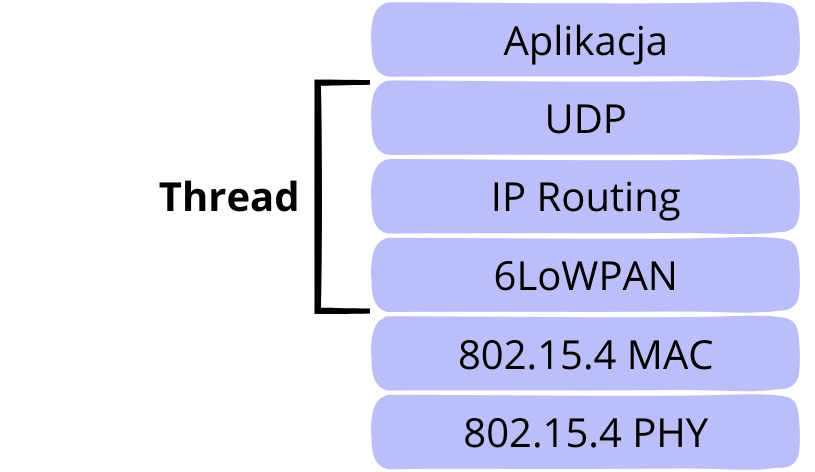
\includegraphics[width=0.8\linewidth]{graphics/thread-protocol-stack.png}
        \caption{Stos protokołów Thread.}
        \label{fig:thread-sprotocol-stack}
    \end{figure}

    \subsection{Warstwa Fizyczna oraz Warstwa Łącza Danych}

        Protokół Thread jest stworzony dla urządzeń, których 2 pierwsze warstwy modelu OSI są oparte o standard definiujący LR-WPAN (ang. \textit{Low-Rate Wireless Personal Area Network}) w wersjach 802.15.4-2006 lub 802.15.4-2015. Jednakże nie jest wymaganym aby urządzenia Thread funkcjonowały w sieciach LR-WPAN. Ponadto protokół Thread nie wykorzystuje zdefiniowanych w 802.15.4 ról, takich jak:
        \begin{itemize}
            \item FFD (ang. \textit{Full-Function Device}),
            \item RFD (ang. \textit{Reduced-Function Device}),
            \item Koordynatora PAN (ang. Personal \textit{Area Network Coordinator}).
        \end{itemize}

    \subsection{Warstwa Sieciowa}

        W warstwie 3. Modelu OSI Thread implementuje protokół IPv6.
        
        W celu umożliwienia przesyłania pakietów IPv6 nad WPAN, wprowadzono warstwę adaptacyjną 6LoWPAN. Usprawnienie to pozwala na enkapsulacje pakietów IPv6 do IEEE 802.15.4 MSDU (MAC Service Data Unit) oraz definiuje mechanizmy kompresji nagłówków IPv6, fragmentacji i składania pakietów IPv6, odpowiednio do oraz z IEEE 802.15.4 MSDU.
        
        Do rutowania (ang. routing) Thread wykorzystuje zdefiniowany w rozdziale 5.9 dokumentacji \cite{thread-1.3.0} protokół rutingu wektora odległości.

    \subsection{Warstwa Transportowa}
    
        Do komunikacji między węzłami w warstwie transportowej, sieć Thread wykorzystuje UDP (ang. \textit{User Datagram Protocol}). Protokół ten jest wymagany przy implementacji stosu Thread, ponieważ jest on wykorzystywany w procesach sygnalizacyjnych oraz mechanizmach zarządzania siecią Thread.
    
        Wdrożenie TCP (ang. \textit{Transport Control Protocol}) nie jest obligatoryjne. Natomiast w przypadku potrzeby uwzględnienia TCP, Thread definiuje wskazówki do efektywnej implementacji tego protokołu w rozdziale 6.2 dokumentacji \cite{thread-1.3.0}.

\section{Typy urządzeń oraz role}

    Niniejsza sekcja ma na celu objaśnienie podstawowych ról węzłów w sieci Thread oraz terminologii, wykorzystywanej w opisywaniu mechanizmów sieci.

    \subsection{Podstawowe role urządzeń}

    W celu pełnej klasyfikacji węzłów w sieci Thread, dokonano ich podziału ze względu na umiejętność przekazywania (ang. \textit{forwarding}) pakietów oraz opisano ich charakterystykę:
    \begin{enumerate}
        \item Ruter (ang. \textit{router}):
        \begin{itemize}
            \item posiada możliwość przekazywania pakietów między węzłami sieci
            \item odbiornik urządzenia pozostaje włączony cały czas,
            \item jest niezbędnym elementem w procesie dołączania innego urządzenia do sieci Thread.
        \end{itemize}
        \item Urządzenie końcowe, ED (ang. \textit{End Device}):
        \begin{itemize}
            \item nie posiada możliwości przekazywania pakietów do innych węzłów,
            \item może komunikować się bezpośrednio tylko z sąsiadującym Ruterem,
            \item odbiornik urządzenia może zostać wyłączony w celu ograniczenia zużycia mocy.
        \end{itemize}
    \end{enumerate}

    ED, stanowiące rolę Dziecka (ang. \textit{Child}), pozostaje zawsze połączone z wyłącznie jednym Ruterem, którego określa się Rodzicem (ang. \textit{Parent} lub \textit{Parent Router}).

    \subsection{Typy urządzeń}

        Ostatecznie, dokonano podziału urządzeń Thread, wyszczególniając dwa główne typy:
        \begin{enumerate}
            \item FTD (ang. \textit{Full Thread Device}),
            \item MTD (ang. \textit{Minimal Thread Device}).
        \end{enumerate}

        Pełną klasyfikację urządzeń w sieci Thread, z kryterium podziału ze względu na typ, przedstawiono na Rys 1.2..

        \subsubsection{Full Thread Device}

            FTD mogą funkcjonować w sieci zarówno w roli Urządzeń Końcowych, jak i w roli Ruterów. Dalej można wyszczególnić: 
            \begin{itemize}
                \item Ruter (ang. \textit{Router}) - urządzenie pełniące wspomnianą rolę Rutera.
                \item REED (ang. \textit{Router Eligible End Device}) - rodzaj Urządzenia Końcowego, które może zostać awansowane do roli Rutera.
                \item FED (ang. \textit{Full End Device}) - rodzaj Urządzenia Końcowego, które nie może zostać awansowane do roli Rutera.
            \end{itemize}
        
        \subsubsection{Minimal Thread Device}

            MTD ograniczone są jedynie do pełnienia roli Urządzeń Końcowych. Kolejno można wyróżnić:
            \begin{itemize}
                \item MED (ang. \textit{Minimal End Device}) - rodzaj Urządzenia Końcowego, którego odbiornik jest zawsze włączony.
                \item SED (ang. \textit{Sleepy End Device}) - rodzaj Urządzenia Końcowego, którego odbiornik jest wyłączony przez większość czasu, natomiast włącza się okazjonalnie, aby otrzymać pakiety przekazane od Rodzica.
            \end{itemize}

        \begin{figure}[H]
            \centering
            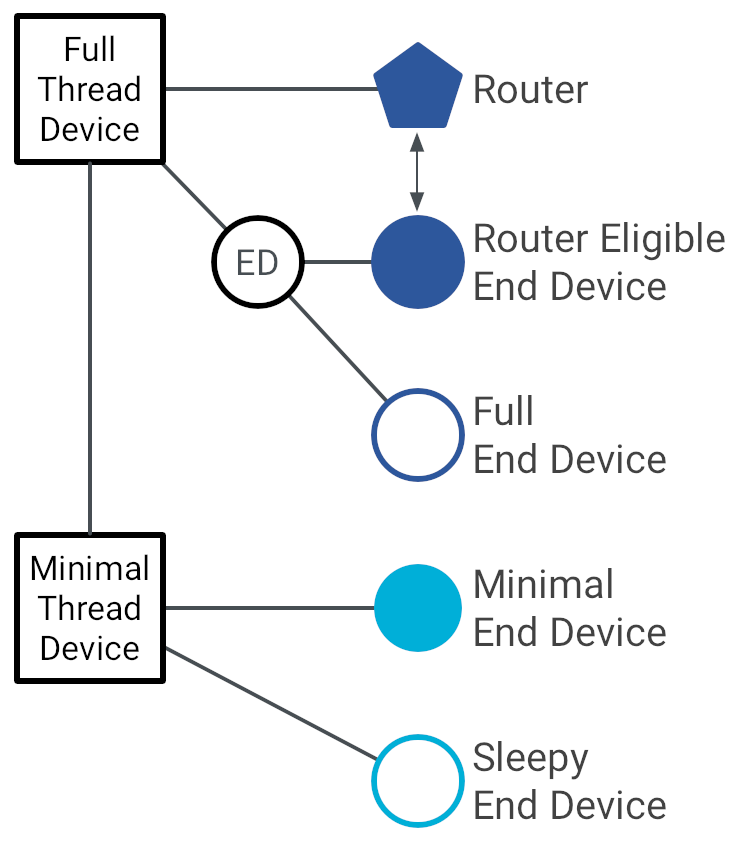
\includegraphics[width=0.8\linewidth]{graphics/ot-primer-taxonomy.png}
            \caption{Podział urządzeń w sieci Thread ze względu na typ \cite{ot-devices}.}
            \label{fig:thread-device-taxonomy}
        \end{figure}

    \subsection{Dodatkowe role Rutera}

        Poza podstawową funkcjonalnością, jaką jest przekazywanie pakietów między węzłami sieci, Ruter w sieci Thread może posiadać dodatkowe role. Między innymi są to:
        \begin{itemize}
            \item Lider (ang. \textit{Leader}),
            \item Ruter Brzegowy (ang. Border Router).
        \end{itemize}

        \subsubsection{Lider}

        Topologia sieci Thread jest dynamiczna i role poszczególnych węzłów zmieniają się w czasie. Za mechanizm awansu ED do Ruterów oraz degradacji Ruterów do ED odpowiada Ruter pełniący rolę Lidera. Opisane zachowanie jest istotne w momencie wystąpienia awarii, gdy jeden z węzłów nie może pełnić swojej roli. Taka cecha sieci nazywana jest samoleczeniem (ang. \textit{self-healing}) i jest charakterystyczna dla sieci kratowych Thread.

        Główne funkcje Lidera:
        \begin{itemize}
            \item Awans do Ruterów oraz ich degradacja poprzez zarządzanie numerem ID Rutera (ang. \textit{Router ID}),
            \item Zbierania i rozsyłanie informacji o sieci Thread (ang. \textit{Thread Network Data})
        \end{itemize}

        Proces awansu i degradacji węzłów przez Lidera uwzględnia możliwości typów urządzeń opisane w sekcji 1.2. W jednej sieci Thread rolę Lidera może pełnić tylko jedno urządzenia. W momencie tworzenie topologii, urządzenie FTD inicjujące sieć zostaje wybierane na Lidera.
        
        \subsubsection{Ruter Brzegowy}

        W celu nawiązania komunikacji między siecią Thread a siecią IP spoza tej domeny, np. Ethernet lub IEEE 802.11, niezbędnym jest, aby w sieci przynajmniej jeden Ruter funkcjonował jako Ruter Brzegowy. Posiada on minimum 2 interfejsy sieciowe, jeden interfejs sieciowy Thread oraz drugi zewnętrzny oparty o IP, najczęściej Ethernet lub WLAN (ang. \textit{Wireless Local Area Network}, oraz potrafi przekazywać między nimi pakiety IPv6.

    Wymienione role Rutera mogą się nakładać. Jeden węzeł może być np. Ruterem Brzegowym, Liderem oraz Rodzicem dla innego ED.

\section{Przegląd wybranych mechanizmów sieci Thread}

    \subsection{Tworzenie sieci}

    Formowanie sieci Thread rozpoczyna się od wybrania IEEE 802.15.4 numeru kanału (ang. \textit{channel}) oraz IEEE 802.15.4 PAN ID (ang. \textit{Personal Area Network Identifier}). Kolejno, aby stworzyć się, urządzenie inicjujące jest zobligowane do wybrania wartości poniższych parametrów:
    \begin{itemize}
        \item Thread Network Short PAN Identifier (PAN ID) - 16 b, liczba całkowita bez znaku, unikalna w zasięgu skanowania.
        \item Network Key - 16 B, do zastosowań kryptograficznych.
        \item Commissioning Credential - 8-255 B, ciąg znaków, wykorzystywany do tworzenia klucza PSKc podczas procesu Commissioning.
        \item Mesh-Local Prefix - prefix IPv6, wykorzystywany do adresacji urządzeń urządzeń w sieci Thread.
        \item Extended PAN ID - 8 B, identyfikuje sieć Thread w zasięgu.
        \item Network Name - 1-16 B, ciąg znaków, identyfikuje sieć Thread.
    \end{itemize}{}

    Urządzenie inicjujące sieć zostaje Ruterem, wybierając dla siebie RouterId, a w konsekwencji braku innych Ruterów w sieci również Liderem.

    \subsection{Commissioning}

    Commissioning to proces pozwalający nowym urządzeniom na dołączenie do istniejącej sieci Thread. W celu zapewnienia bezpieczeństwa oraz powstrzymanie niechcianych urządzeń (ang. Rouge Device) przed połączeniem z siecią Thread, węzły powinny zostać uwierzytelnione i autoryzowane. Podstawą działania mechanizmu jest protokół DTLS (ang. \textit{Datagram Transport Layer Security}).

    W celu opisania mechanizmu Commissioning, wprowadzono następujące terminy:
    \begin{itemize}
        \item Joiner - rola nowego urządzenia próbującego podłączyć się do sieci.
        \item Commissioner - rola urządzenia, który uwierzytelnia węzeł o roli Joiner.
        \item Joiner Router - rola urządzenia, który jest Ruterem i znajduje się najbliżej sieci, do której stara się przyłączyć Joiner.
    \end{itemize}

    Ze względu na to czy Commissioner znajduje się w sieci Thread lub poza nią, wyróżniamy kolejno 2 typy procesu Commissioning \cite{thread-commissioning}:
    \begin{enumerate}
        \item On-mesh,
        \item External.
    \end{enumerate}

    W aktualnej sekcji, opisany zostanie jedynie scenariusz On-mesh, w którym Commissioner jest częścią sieci w domenie Thread.

    Na Rys. 1.3. przedstawiono przykładową sieć Thread z wyszczególnieniem ról charakterystycznych dla procesu On-mesh Commissioning.

    Urządzenia, które mogą pełnić rolę Commissioner, wymieniają wiadomości z Liderem, w celu ustalenia, który z kandydatów będzie pełnił tę funkcję. W sieci Thread, w jednym momencie może istnieć dokładnie jeden Commissioner. Proces ten określono nazwą Petitioning.

    Po elekcji urządzenia, który będzie pełnił rolę Commissioner, kolejne urządzenia Joiner są w stanie rozpocząć próbę dołączenia do sieci, nazwaną Joining.
    W kolejnym kroku zestawione zostaje połączenie Joiner-Joiner Router, a następnie Joiner-Commissioner, które jest zabezpieczone z użyciem protokołu DTLS i do którego zestawienia niezbędne jest Joining Device Credential (PSKd). Następnie Joiner zostaje uwierzytelniony na skutek wymiany kolejnych wiadomości z Commissioner. W wyniku poprawnie przeprowadzonego procesu Commissioning urządzenie posiada niezbędne informacje aby podłączyć się do sieci.

    \begin{figure}[H]
        \centering
        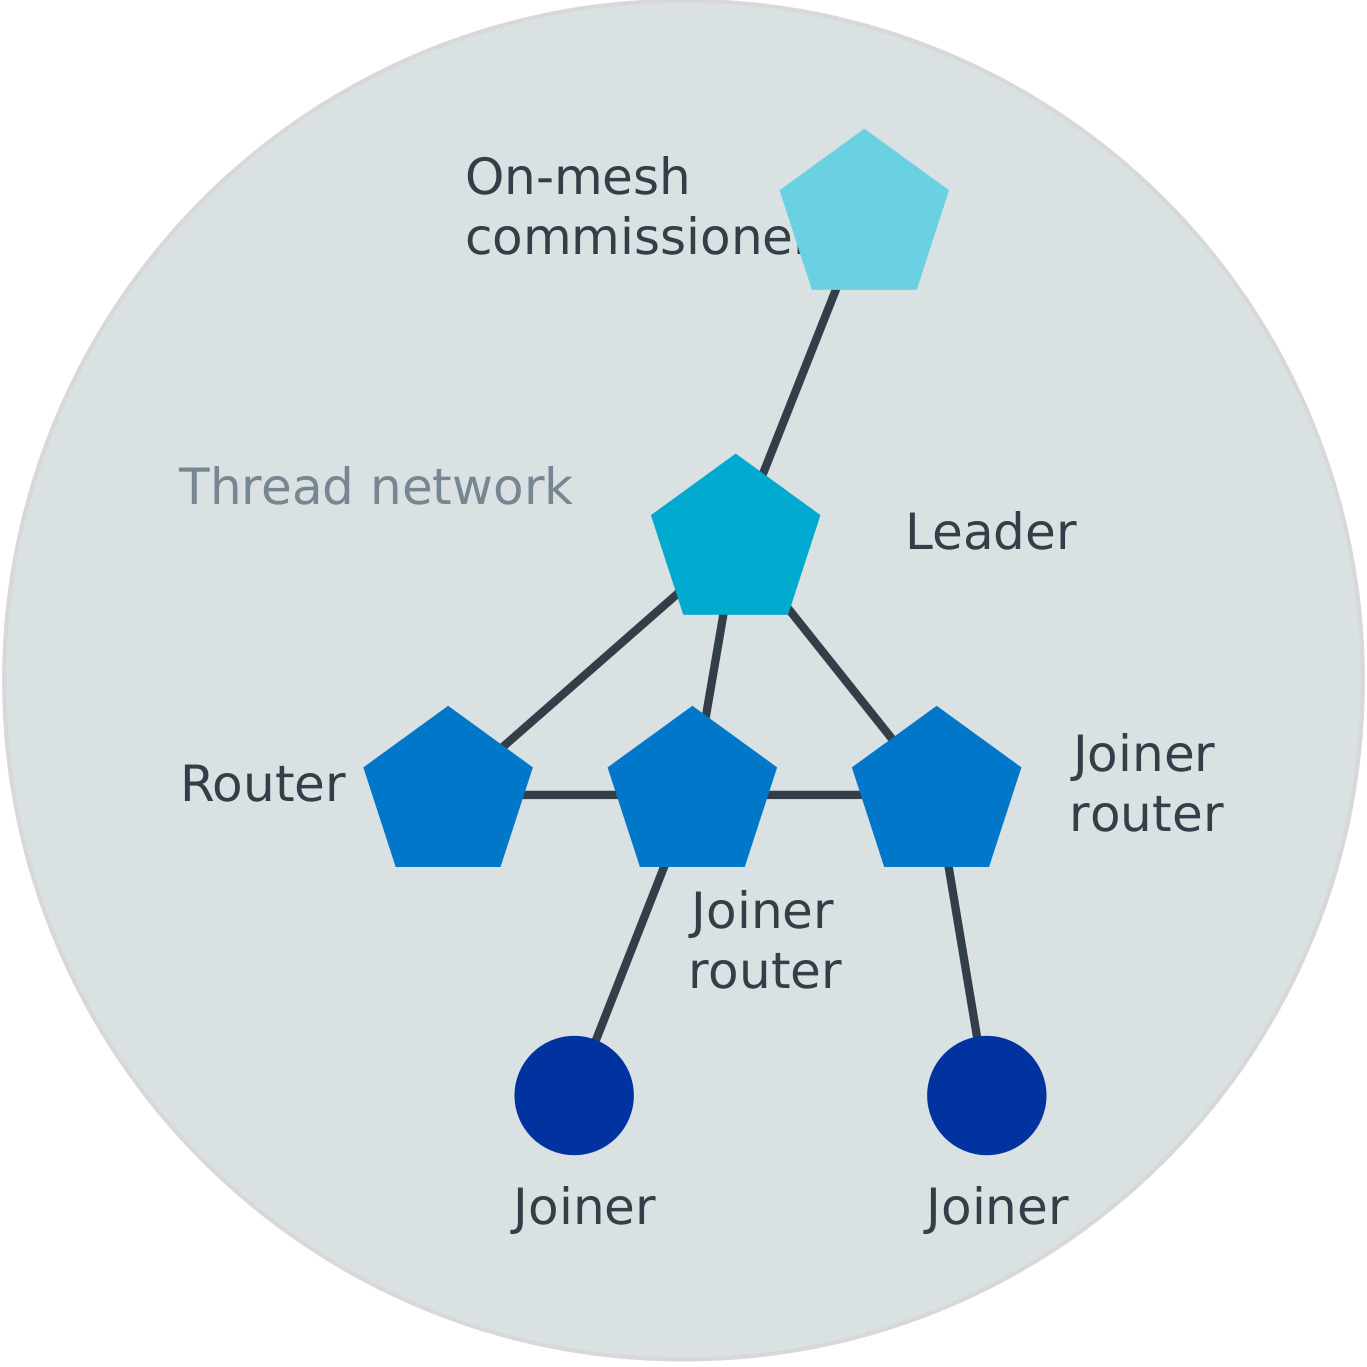
\includegraphics[width=0.8\linewidth]{graphics/Thread_on-mesh_commissioning.jpg}
        \caption{Przykładowa topologia sieci Thread podczas procesu On-mesh Commissioning \cite{thread-commissioning}.}
        \label{fig:thread-on-mesh-commissioning}
    \end{figure}

    \subsection{Dołączanie do sieci}

    Proces dołączania do sieci Thread rozpoczyna się od skanowania istniejących sieci IEEE 802.15.4 na kolejnych kanałach. Urządzenie podłączające się rozgłasza żądanie Beacon Request. W przypadku otrzymania wiadomości przez Rutery lub REED, odpowiadają one poprzez wysłanie Beacon, który zawiera podstawowe informacje na temat danej sieci.

    Po zakończeniu procesu odkrywania sieci Thread, urządzenie może próbować podłączyć się do istniejącej sieci lub utworzyć własną.

    Aby urządzenie było w stanie dołączyć do sieci Thread, jest zobowiązane do pozyskania poniższych parametrów opisujących konkretną sieć Thread:
    \begin{itemize}
        \item Network Key,
        \item PSKc,
        \item Mesh-Local Prefix,
        \item Extended PAN ID,
        \item Network Name.
    \end{itemize}
    
    Informacje te mogą zostać uzyskane w wyniku pomyślnego zakończenia procesu Commissioning.

    Urządzenie posiadający wszystkie niezbędne informacje o sieci, w kolejnym kroku zestawia połączenie Dziecko-Rodzic z wykorzystaniem mechanizmu MLE (Mesh Link Establishment). Ostatecznie, nawiązanie połączenia zakończone jest przesłaniem przez Rodzica identyfikatora Child ID. Od tego momentu urządzenie dołączające jest częścią sieci Thread.

















\chapter{Propozycja systemu}
\label{cha:propozycja-systemu}

Na Rysunku \ref{fig:system-architecture} przedstawiono system automatyki domowej, którego projekt i implementacja leży w zakresie kolejnych rozdziałów.

\begin{figure}[H]
    \centering
    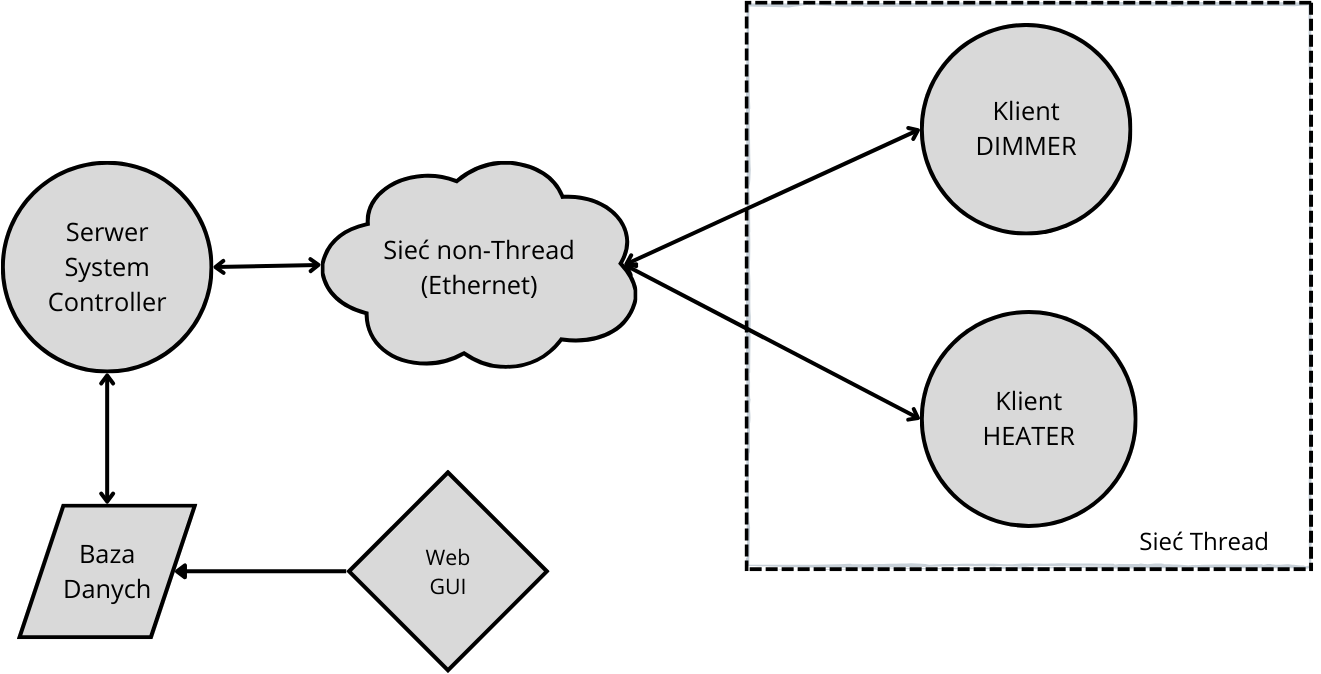
\includegraphics[width=0.8\linewidth]{graphics/system-architecture.png}
    \caption{Proponowana architektura systemu automatyki domowej.}
    \label{fig:system-architecture}
\end{figure}

W dalszej części pracy, termin \textit{parametr regulacji}, będzie odnosił się do procentowego stosunku aktualnej mocy układu regulacji do jego maksymalnej wartości mocy.

Funkcją systemu jest utrzymanie zdefiniowanych w Tabeli \ref{tab:profiles-parameters} parametrów środowiska, na poziomie zadanym przez użytkownika systemu. W tym celu urządzenia systemu dokonują pomiaru parametrów oraz regulacji swojej mocy.

\begin{table}[H]
    \centering
    \caption{Zestaw parametrów określonych dla zdefiniowanych profili.}
    \begin{tabular}{|c|c|c|}
         \hline
         \rowcolor{gray!20}
          & HEATER & DIMMER \\
         \hline
         \cellcolor{gray!20}Parametr & temperatura & natężenie oświetlenia \\
         \hline
         \cellcolor{gray!20}Jednostka & $^{\circ}$C & lux \\
         \hline
    \end{tabular}
    \label{tab:profiles-parameters}
\end{table}

Zaproponowany system opiera się o architekturę klient-serwer i składa się z 5 funkcjonalnych bloków:
\begin{enumerate}
    \item klienta Dimmer,
    \item klienta Heater,
    \item serwera z aplikacją System Controller,
    \item Bazy Danych,
    \item Web GUI (ang. \textit{Graphical User Interface}).
\end{enumerate}

Celem niniejszego rozdziału jest omówienie zaproponowanego systemu oraz opisanie jego poszczególnych komponentów. 

\section{Strona kliencka}
\label{sec:system-clients}

Klientami w systemie są urządzenia połączone w sieć Thread, realizujące profile określone w Tabeli \ref{tab:profiles-parameters}. Rolą HEATER oraz DIMMER jest implementacja usług pomiaru i regulacji, odpowiednio, temperatury oraz natężenia oświetlenia.
Klienci komunikują się z serwerem w celu dostarczenia pomiarów oraz uzyskania informacji o decyzji dotyczącej konieczności regulacji mocy.
    
\section{Strona serwera}

System Controller to aplikacja znajdująca się w sieci spoza domeny Thread, pełniąca rolę serwera. Komponent przetwarza otrzymane wartości aktualnego stanu środowiska i uwzględniając zadane przez użytkownika wartości, dokonuje decyzji odnośnie regulacji. Ostatecznie aplikacja powiadamia klientów HEATER oraz DIMMER o konieczności zmiany parametru regulacji.

Dodatkowo System Controller odpowiedzialny jest za logowanie otrzymanych wartości aktualnego stanu parametrów oraz podjęte decyzje odnośnie regulacji.

\section{Sterowanie i logowanie}

W celu zadania wartości parametrów, do których powinien dążyć system, użytkownik korzysta z Web GUI. Graficzny interfejs umożliwia zdefiniowanie stanu, jak również wgląd do logów systemu.

Wpisy systemowe oraz zadeklarowany stan parametrów użytkownika, przechowywane są w bazie danych, do której dostęp ma zarówno Web GUI, jak i System Controller.
\chapter{Wykorzystane narzędzia}
\label{cha:narzedzia}

Celem obecnego rozdziału jest opisanie wykorzystanych do implementacji systemu narzędzi, takich jak platforma sprzętowa, biblioteki programowe, środowisko programistyczne.

\section{Platforma sprzętowa nRF52833}

Do projektu wykorzystano układ Nordic Semiconductor nRF52833 z serii nRF52.

\subsection{Charakterystyka układu}

    Platforma nRF52833 to SoC (ang. \textit{System on Chip}) wyposażony w 64 MHz CPU (ang. \textit{Central Processing Unit}) z rdzeniem z rodziny ARM Cortex-M4 oraz jednostką FPU (ang. \textit{Floating Point Unit}) \cite{nrf52833-characteristics}.
    Układ posiada 512 kB pamięci nieulotnej flash oraz 128 kB pamięci operacyjnej RAM (ang. \textit{Random Access Memory}).

    SoC zawiera radiowy układ nadawczo-odbiorczy (ang. \textit{Transreceiver}), umożliwiający odbiór ramek IEEE 802.15.4-2006, co jest kluczowe do uruchomienia aplikacji działającej na stosie Thread.

    Według zapewnień producenta platforma nRF52833 może zostać wykorzystana do zastosowań Smart-Home lub przemysłowego IoT i pracować jako czujnik, lub kontroler \cite{nrf52833-characteristics}.

    Do procesu rozwijania oprogramowania, wykorzystano płytkę ewaluacyjną nRF52833 DK, której schemat blokowy przedstawiono na Rysunku \ref{fig:nrf8233-block-diagram}.

    \begin{figure}[H]
        \centering
        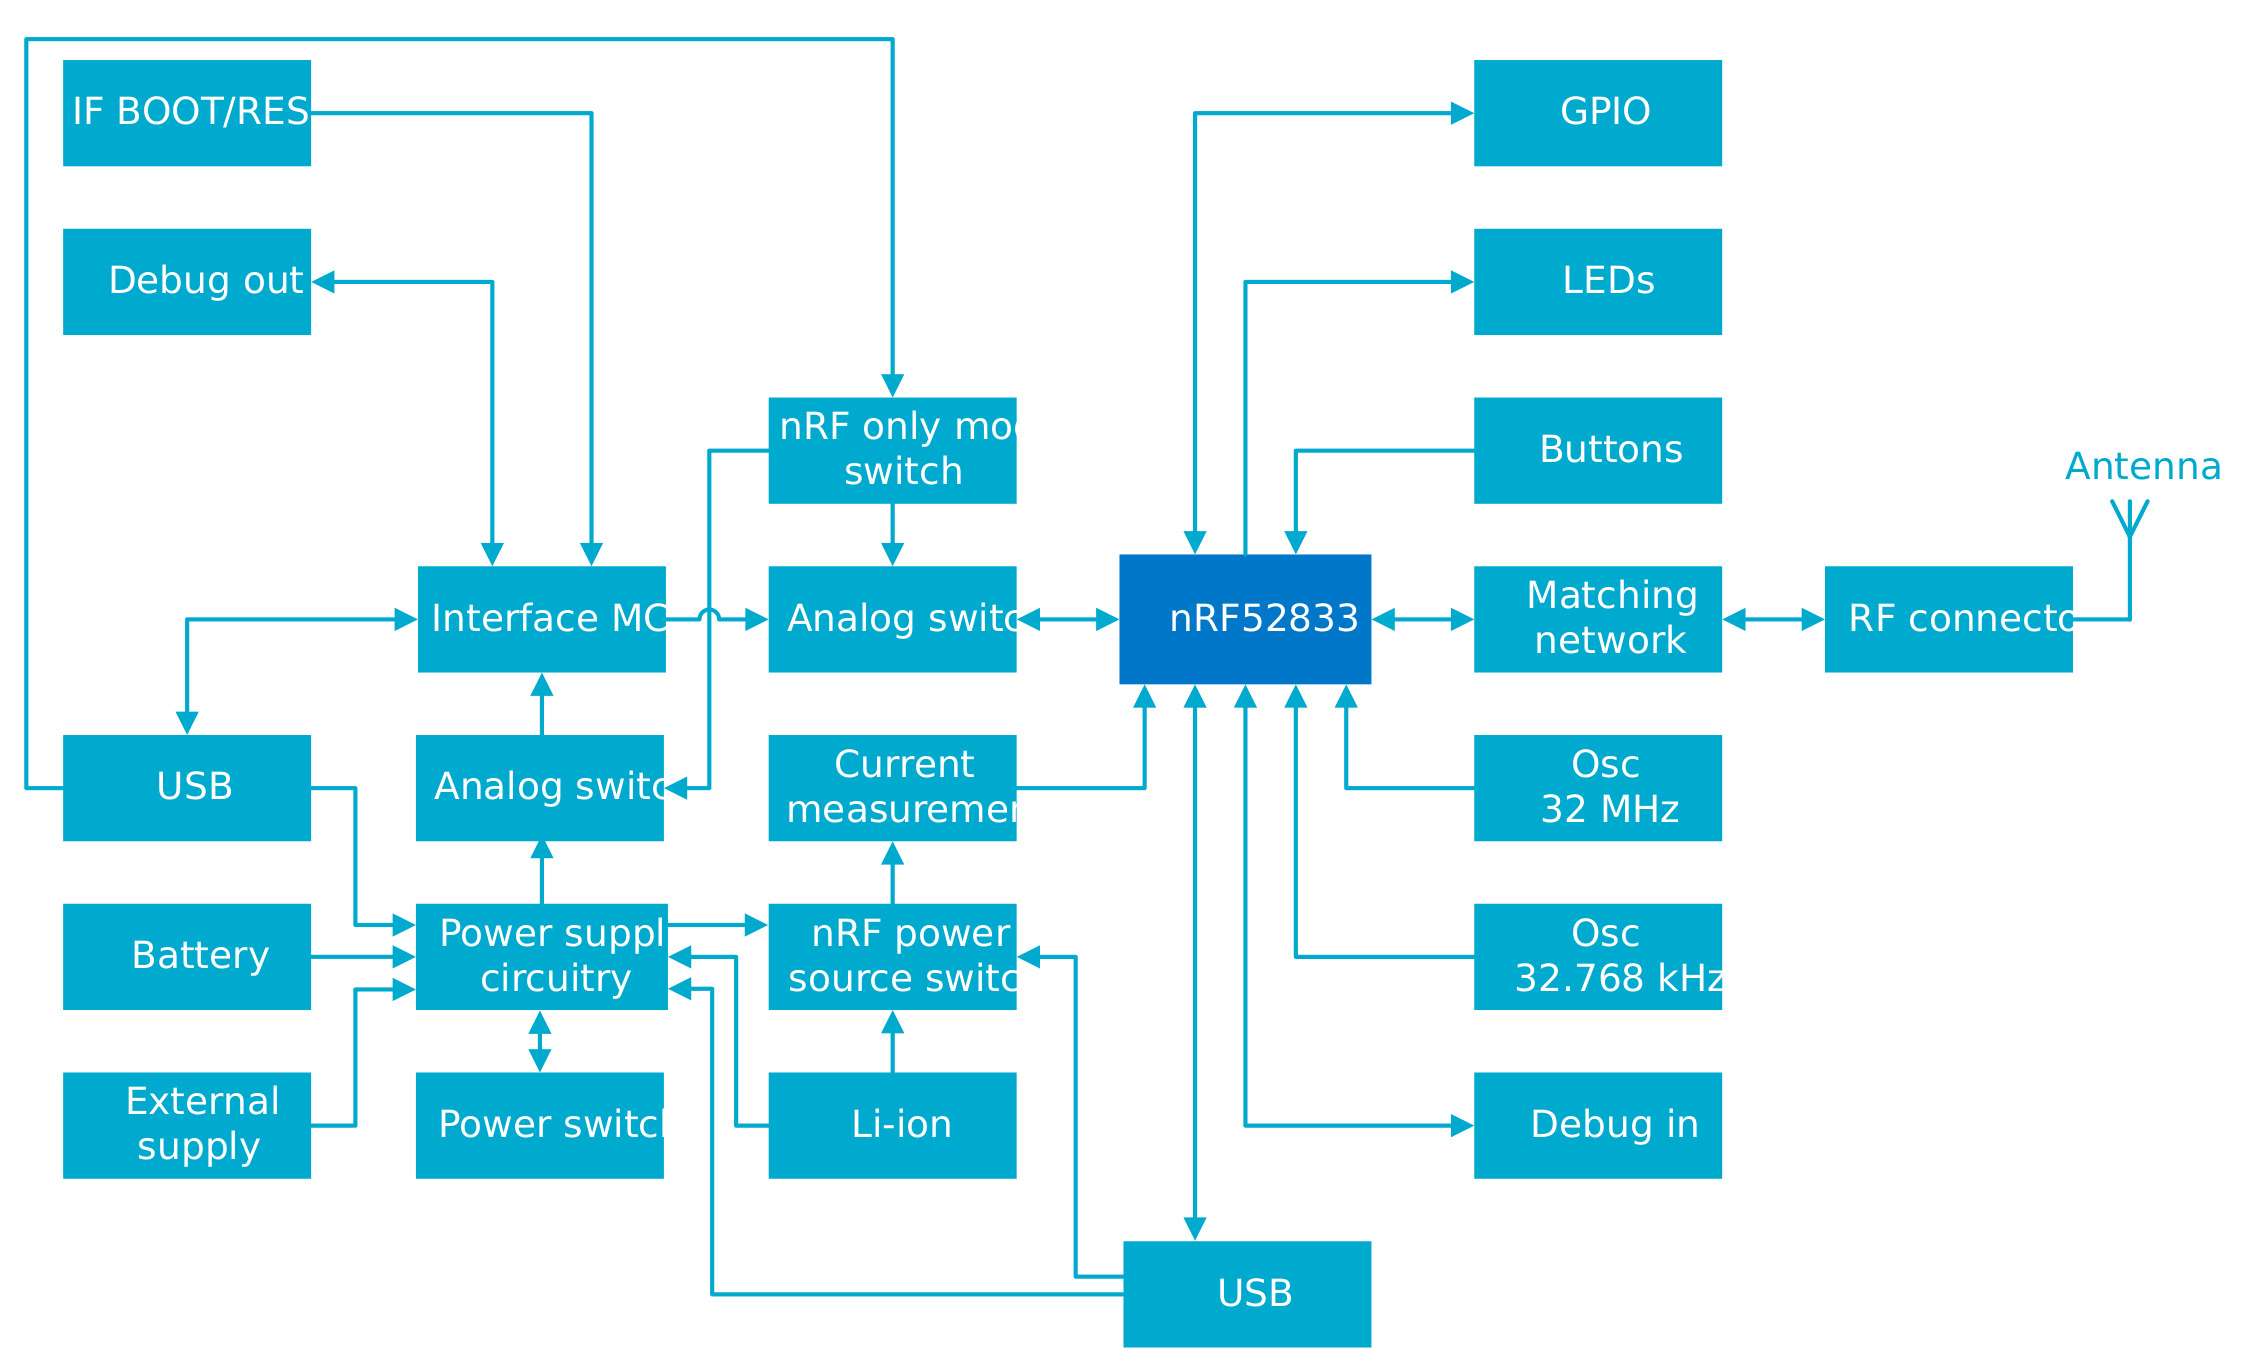
\includegraphics[width=0.8\linewidth]{graphics/external/nrf52833DK_block_diagram.jpg}
        \caption{Schemat blokowy płytki ewaluacyjnej nRF52833 DK \cite{nrf52833-diagram}.}
        \label{fig:nrf8233-block-diagram}
    \end{figure}

\subsection{Narzędzia producenta}
\label{subsec:producer-tools}

    Do tworzenia oprogramowania wykorzystano zestaw narzędzi nRF Connect SDK \cite{nrf-connect}. Stworzone przez Nordic Semiconductor SDK (ang. \textit{Software Development Kit}) jest dedykowane do tworzenia aplikacji, wykorzystujących transmisję bezprzewodową małej mocy. nRF Connect SDK opiera się między innymi, na urządzeniach z serii nRF52 oraz wspiera rozwój oprogramowania w środowisku Microsoft Windows.

    nRF Connect SDK udostępnia system operacyjny czasu rzeczywistego Zephyr oraz przykładowe kody źródłowe aplikacji na nim opartych. Ponadto zestaw narzędzi integruje szereg bibliotek i sterowników z zakresu komunikacji bezprzewodowej, które umożliwiają przyjazne użytkownikowi wdrożenie we własnych aplikacjach, a w szczególności dotyczące technologii:
    \begin{itemize}
        \item Thread,
        \item CoAP (ang. \textit{Constrained Application Protocol}),
        \item IPv6,
        \item UDP,
        \item IEEE 802.15.4.
    \end{itemize}

    W projekcie systemu wykorzystano nRF Connect SDK w wersji 2.4.0.

    Podczas tworzenia oprogramowania, użyto również zapewnione przez Nordic Semiconductor rozszerzenie do edytora tekstu Visual Studio Code \cite{nrf-ide}, który umożliwia tworzenie, konfigurowanie i budowanie aplikacji dedykowanych dla platform Nordic Semiconductor oraz debugowanie i programowanie urządzeń z serii nRF52. 

\section{Openthread}

    OpenThread to upubliczniona, oparta na licencji BSD-3 implementacja stosu Thread, stworzona przez Google. Projekt OpenThread jest wspierany przez, między innymi, Nordic Semiconductor. Stos OpenThread wraz z platformą sprzętową nRF52833 posiada certyfikat \textit{Thread Certified Component} \cite{nrf52833-tcc}, co świadczy o pełnej zgodności ze standardem Thread oraz spełnieniu dodatkowych wymogów wyszczególnionych w specyfikacji \cite{thread-1.3.0}. Implementacja OpenThread wraz z API (ang. \textit{Application Programming Interface}) jest uwzględniona w nRF Connect SDK przedstawionym w podsekcji \ref{subsec:producer-tools}.

    Poza implementacją stosu Thread OpenThread dostarcza dodatkowe narzędzia pomocne przy rozwoju systemów opartych o implementację Thread. Jednym z nich jest aplikacja Rutera Brzegowego OTBR (ang. \textit{OpenThread Border Router}) \cite{openthread-br}.
\chapter{Implementacja systemu}
\label{cha:implementacja}

Celem omawianego rozdziału jest przedstawienie implementacji proponowanego w Rozdziale \ref{cha:propozycja-systemu} systemu automatyki domowej. Niniejsza część została podzielona na dwie sekcje. W pierwszej sekcji zaprezentowana zostanie stworzona na potrzeby projektu sieć Thread. Kolejny fragment poświęcony jest warstwie aplikacji, technologiom wykorzystanym przy wdrażaniu komponentów oraz zasadzie działania systemu.

Projekt aplikacji systemu znajduje się w stworzonym przez autora pracy repozytorium \cite{project-repo}.

\section{Sieć Thread}

    \subsection{Założenia}
    \label{sec:thread-network-assumptions}
    
        Do stworzenia sieci Thread wykorzystano 5 urządzeń Nordic Semiconductor nRF52833 oraz Laptop Dell G3 15 z procesorem Intel Core i7 9. generacji, z systemem operacyjnym Microsoft Windows 11. Przed przystąpieniem do procesu implementacji sieci Thread, dokonano następujących założeń:
        \begin{itemize}
            \item Jedna platforma nRF52833 wraz z laptopem Dell zostaną wykorzystane do pełnienia roli Rutera brzegowego.
            \item Dwa urządzenia nRF52833 zostaną skonfigurowane do typu MTD oraz będą stanowiły urządzenia końcowe, MED oraz SED, które w warstwie aplikacji będą pełniły rolę profili HEATER oraz DIMMER.
            \item Dwa urządzenia nRF52833 zostaną skonfigurowane do typu FTD. Zostaną one wprowadzone do sieci, aby zapewnić nadmiarowość i pozwolić Liderowi Thread na dostosowanie topologii do aktualnych potrzeb i wymagań sieci.
        \end{itemize}

        Na Rysunku \ref{fig:thread-topology} przedstawiono przykładową topologię sieci Thread, złożoną z wyszczególnionych powyżej urządzeń.

        \begin{figure}[H]
            \centering
            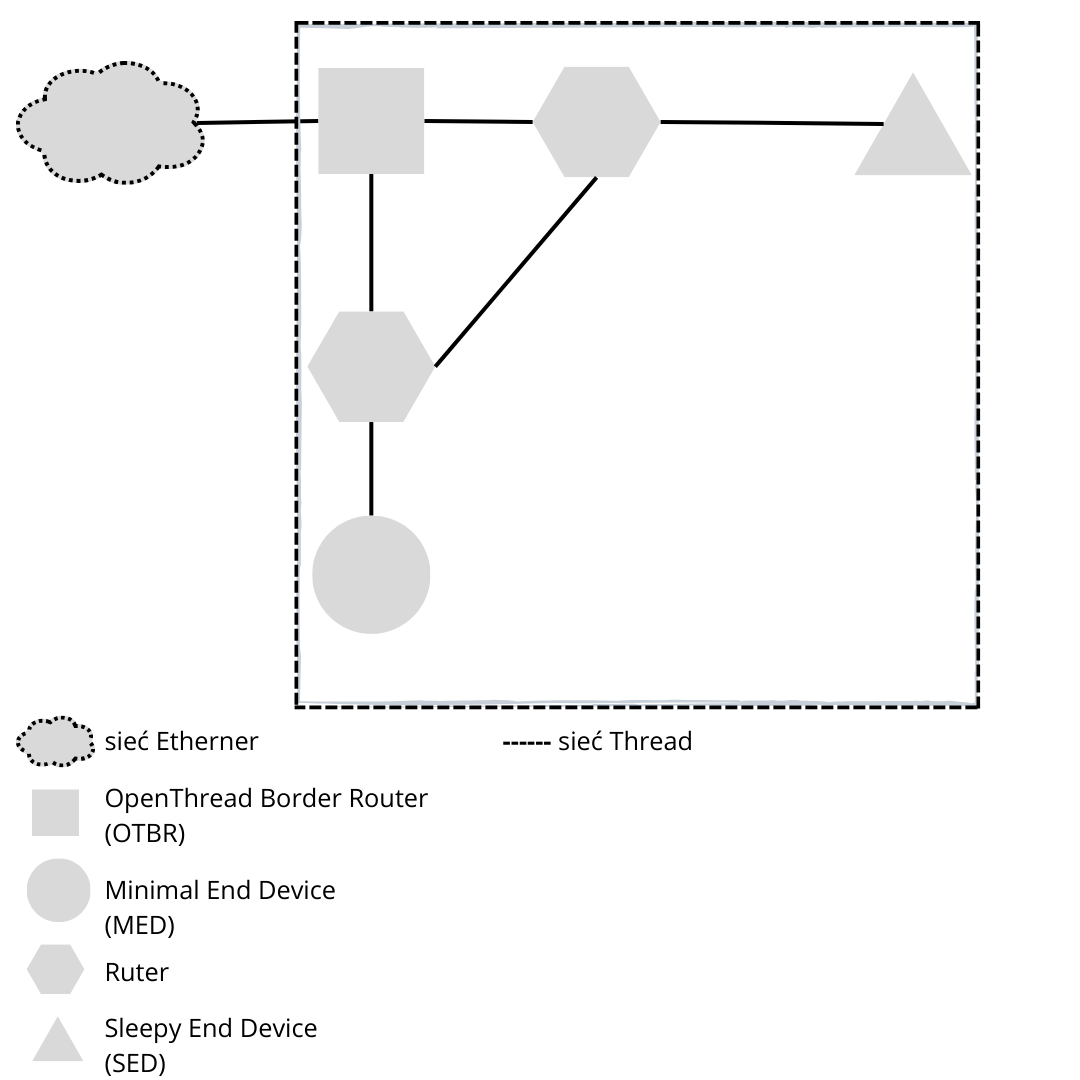
\includegraphics[width=0.8\linewidth]{graphics/thread-topology.png}
            \caption{Przykładowa topologia sieci Thread złożona z urządzeń wymienionych w założeniach w Sekcji \ref{sec:thread-network-assumptions}.}
            \label{fig:thread-topology}
        \end{figure}

    \subsection{Ruter Brzegowy}
    \label{subsec:otbr-implementation}

        W celu zapewnienia komunikacji przyszłej sieci Thread z zewnętrzną siecią Ethernet, w pierwszej kolejności przystąpiono do konfiguracji Rutera brzegowego, wykorzystując implementację OTBR. 
        
        Aplikacja OTBR jest dedykowana dla systemów operacyjnych Linux oraz do poprawnego działania wymaga nawiązania komunikacji zarówno z interfejsem sieci Thread, jak i z interfejsem sieci zewnętrznej. Z tego powodu, w początkowym kroku skonfigurowano platformę Linux jako maszynę wirtualną z dystrybucją Ubuntu tak, aby zapewnić komunikację sieciową oraz komunikację portów szeregowych między urządzeniem gościa (ang. \textit{Guest}) (maszyną wirtualną) a gospodarza (ang. \textit{Host}) (Laptop Dell). Kolejno skonfigurowano środowisko deweloperskie, instalując narzędzia takie jak system kontroli wersji Git oraz IDE (ang. \textit{Integrated Development Environment}). 

        Po weryfikacji poprawności działania maszyny wirtualnej kontynuowano proces konfiguracji OTBR, wykorzystując instrukcję zamieszczoną na oficjalnej stronie projektu OpenThread \cite{otbr-docker}. Zaprogramowano jedno z urządzeń nRF52833 aplikacją RCP (ang. \textit{Radio Co-Processor}), używając dostarczonej przez OpenThread implementacji \cite{otbr-rcp-app}. Ostatecznie zainstalowano oprogramowanie Docker oraz pobrano dystrybuowany przez OpenThread kontener.

        Tak przygotowane środowisko Linux oraz zaprogramowane urządzenie nRF52833 są gotowe do uruchomienia w pełni funkcjonalnej aplikacji Rutera Brzegowego.

    \subsection{Urządzenia MTD oraz FTD}
    \label{subsubsec:mtd-ftd-devices-implementation}

    Aplikację dla 4 pozostałych urządzeń nRF52833 stworzono w języku C z wykorzystaniem nRF Connect SDK oraz środowiska programistycznego nRF Connect IDE. W plikach konfiguracyjnych projektów skonfigurowano odpowiednio stos protokołu i niezbędne funkcjonalności Thread, system logowanie, GPIO (ang. \textit{general-purpose input/output}). Kolejno wybrano tryb MTD dla 2 urządzeń, natomiast dla pozostałych FTD. 

    Co więcej, w urządzeniach MTD uwzględniono możliwość przejścia w tryb energooszczędny, poprzez naciśnięci przycisku Button 3, w wyniku czego ED zmienia pełniącą rolę z MED na SED oraz obniża zużycie energii w wyniku ograniczenia zużycia pamięci RAM.

    Na potrzeby procesu rozwoju oprogramowania, wzbogacono wszystkie 4 platformy, o sygnalizację stanu urządzenia Thread przy pomocy LED (ang. \textit{light-emitting diode}). Dioda LED1 świeci się, gdy urządzenie Thread jest włączone do sieci.
    
\section{Warstwa Aplikacji}

    Do wymiany informacji podczas komunikacji klient-serwer między urządzeniami końcowymi w sieci Thread a System Controllerem, wykorzystano protokół warstwy aplikacji Constrained Application. CoAP jest protokołem opartym o REST API (ang. \textit{Representational State Transfer Application Programming Interface}), który nawiązuje połączenie z wykorzystaniem wspieranego przez stos Thread protokołu UDP.

    \subsection{Implementacja komponentów systemy}

        Obecna sekcja ma za zadanie przybliżyć szczegóły implementacji poszczególnych komponentów wymienionych w Rozdziale \ref{cha:propozycja-systemu}.

        \subsubsection{Baza danych}
            Przez wzgląd na mały rozmiar, pełne wsparcie funkcjonalności SQL (ang. \textit{Structured Query Language}) oraz możliwość przechowywania bazy danych w pojedynczym pliku, jako silnik wykorzystywanej w projekcie systemu Bazy Danych wybrano SQLite. \cite{sqlite}.

            Stworzony na potrzeby systemu zestaw tabel Bazy Danych przedstawiono na Rysunku \ref{fig:db-diagram}.

            \begin{figure}[H]
                \centering
                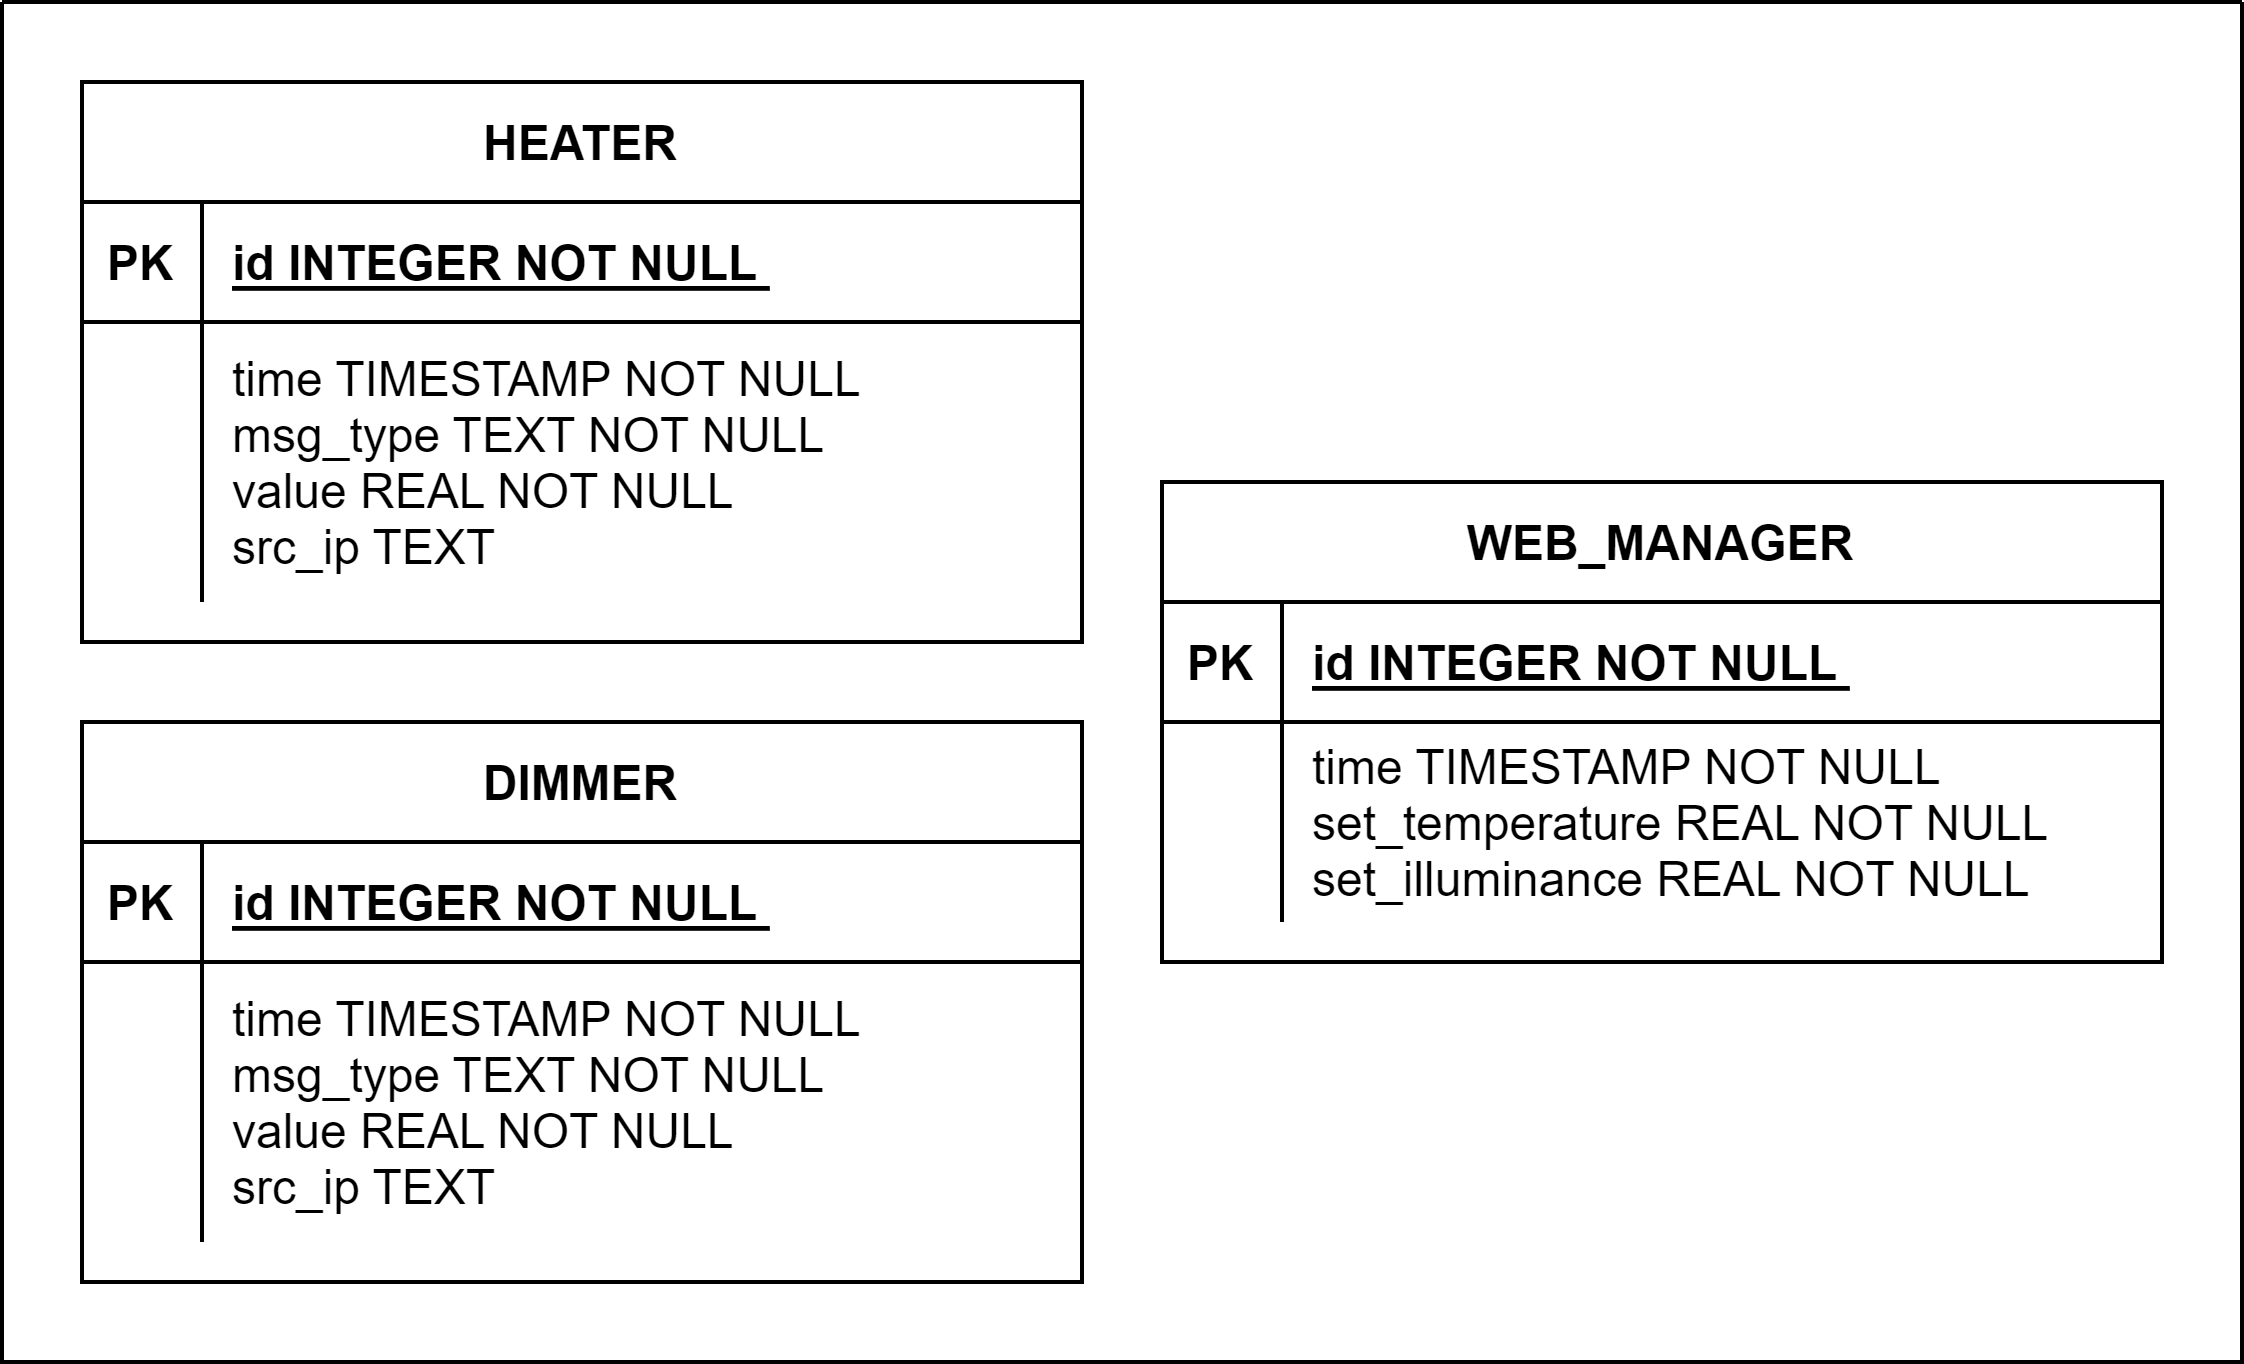
\includegraphics[width=0.8\linewidth]{graphics/db_diagram.png}
                \caption{Schemat tabel Bazy Danych systemu.}
                \label{fig:db-diagram}
            \end{figure}

            Tabela WEB\_MANAGER ma za zadanie przechowywać wpisy dotyczące ustawionych przez użytkownika parametrów. Tablica HEATER oraz tablica DIMMER zawierają informację o kolejnych przetworzonych przez System Controller żądaniach CoAP.
    
        \subsubsection{System Controller}
    
            System Controller został wdrożony jako aplikacja w języku Python, przeznaczona dla urządzeń z systemem operacyjnym Linux.
            System Controller odbiera żądania oraz wysyła odpowiedzi CoAP z wykorzystaniem dostarczonego przez bibliotekę aiocoap API \cite{aiocoap}. URI (ang. \textit{Uniform Resource Identifier}) zdefiniowanych zasobów serwera, obsługiwany typ zapytań oraz ich funkcje, zestawiono w Tabeli \ref{tab:resurces}.
            
            Zarządzanie Bazą Danych SQLite odbywa się z użyciem wbudowanych w język Python bibliotek \textit{sqlite3} oraz \textit{aiosqlite}.

            \begin{table}[H]
                \centering
                \caption{Zasoby serwera CoAP.}
                \begin{tabular}{|l|l|l|}
                     \hline
                     \rowcolor{gray!20}
                     \multicolumn{1}{|c|}{Zasób} & \multicolumn{1}{c|}{Typ zapytań} & \multicolumn{1}{c|}{Funkcja} \\
                     \hline
                     temperature & GET, PUT & Przechowuje wartość aktualnej temperatury środowiska.\\
                     \hline
                     illuminance & GET, PUT & Przechowuje wartość aktualnego natężenia oświetlenia środowiska.\\
                     \hline
                     heater\_regulation & GET & Zwraca wartość parametru regulacji dla układu HEATER.\\
                     \hline
                     dimmer\_regulation & GET & Zwraca wartość parametru regulacji dla układu DIMMER.\\
                     \hline
                \end{tabular}
                \label{tab:resurces}
            \end{table}
    
        \subsubsection{HEATER oraz DIMMER}

            Platformy nRF52833 pracujące jako MTD, w których skonfigurowano stos Thread, jak opisano w Podsekcji \ref{subsubsec:mtd-ftd-devices-implementation}, wzbogacono o warstwę aplikacji. Urządzenia Końcowe symulują zachowanie zdefiniowanych w Sekcji \ref{sec:system-clients} profili HEATER oraz DIMMER. Wysyłanie zapytań oraz odbieranie odpowiedzi CoAP zaimplementowano z wykorzystaniem API dostarczonego przez nRF Connect SDK, oraz OpenThread.

            W urządzeniach HEATER oraz DIMMER skonfigurowano przycisk Button 3, którego naciśnięcie inicjalizuje stronę klienta CoAP oraz pobiera z sieci prefiks NAT64, niezbędny do nawiązania połączenia z serwerem o skonfigurowanym IPv4.
        
        \subsubsection{Web GUI}

            Interfejs użytkownika Web GUI stanowi aplikacja w języku Python, którą stworzono z użyciem następujących technologii webowych:
            \begin{itemize}
                \item mikro-frameworku Flask \cite{flask},
                \item CSS (ang. \textit{Cascading Style Sheets}),
                \item HTML (ang. \textit{HyperText Markup Language}).
            \end{itemize}
            Aplikacja komunikuje się bezpośrednio z bazą danych, wykorzystując bibliotekę sqlite3.

            \begin{figure}[H]
                \centering
                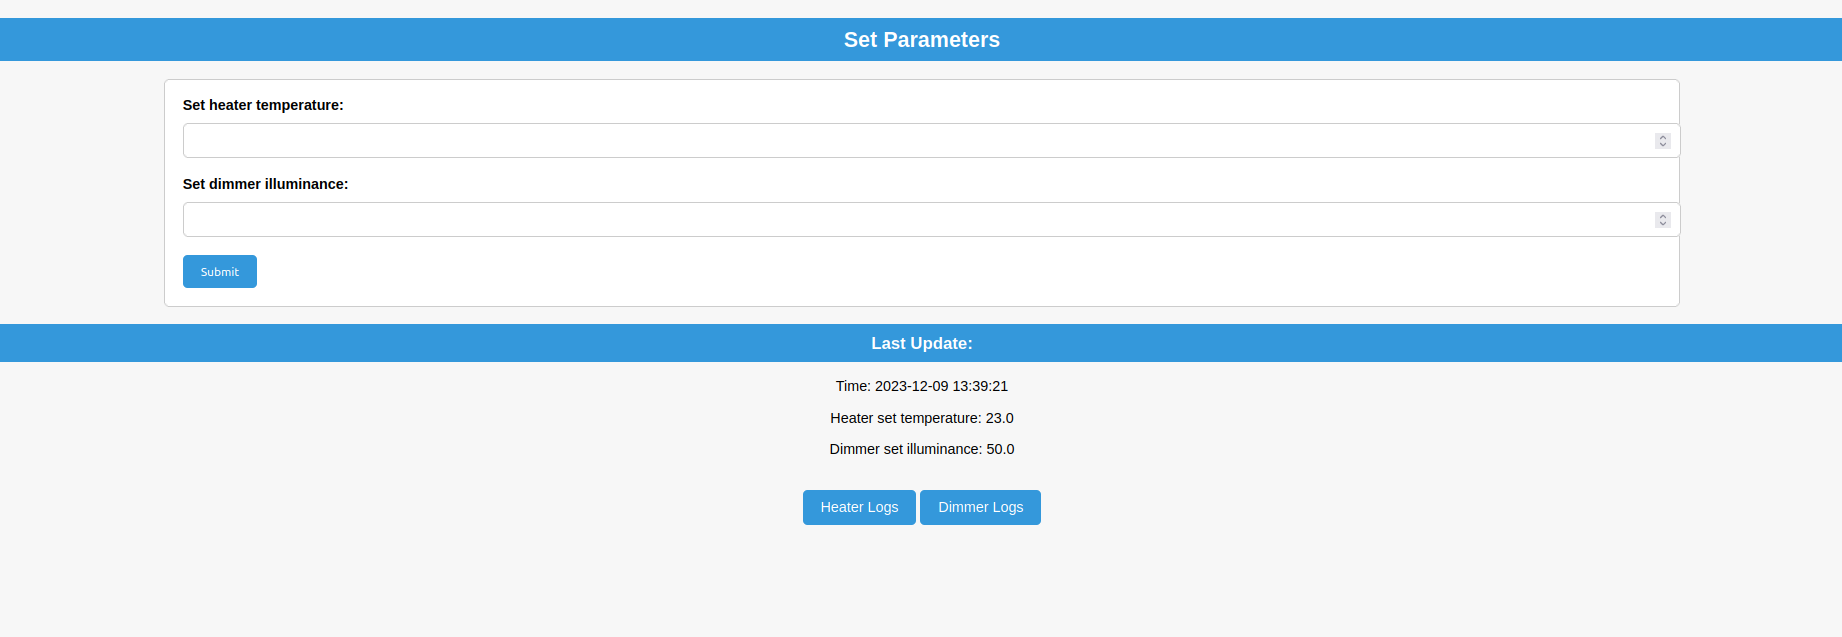
\includegraphics[width=0.8\linewidth]{graphics/screenshots/web-gui-set-parameters.png}
                \caption{Zrzut ekranu przedstawiający panel Web GUI przeznaczony do ustalania parametrów systemu.}
                \label{fig:web-gui-set-parameters}
            \end{figure}

            \begin{figure}[H]
                \centering
                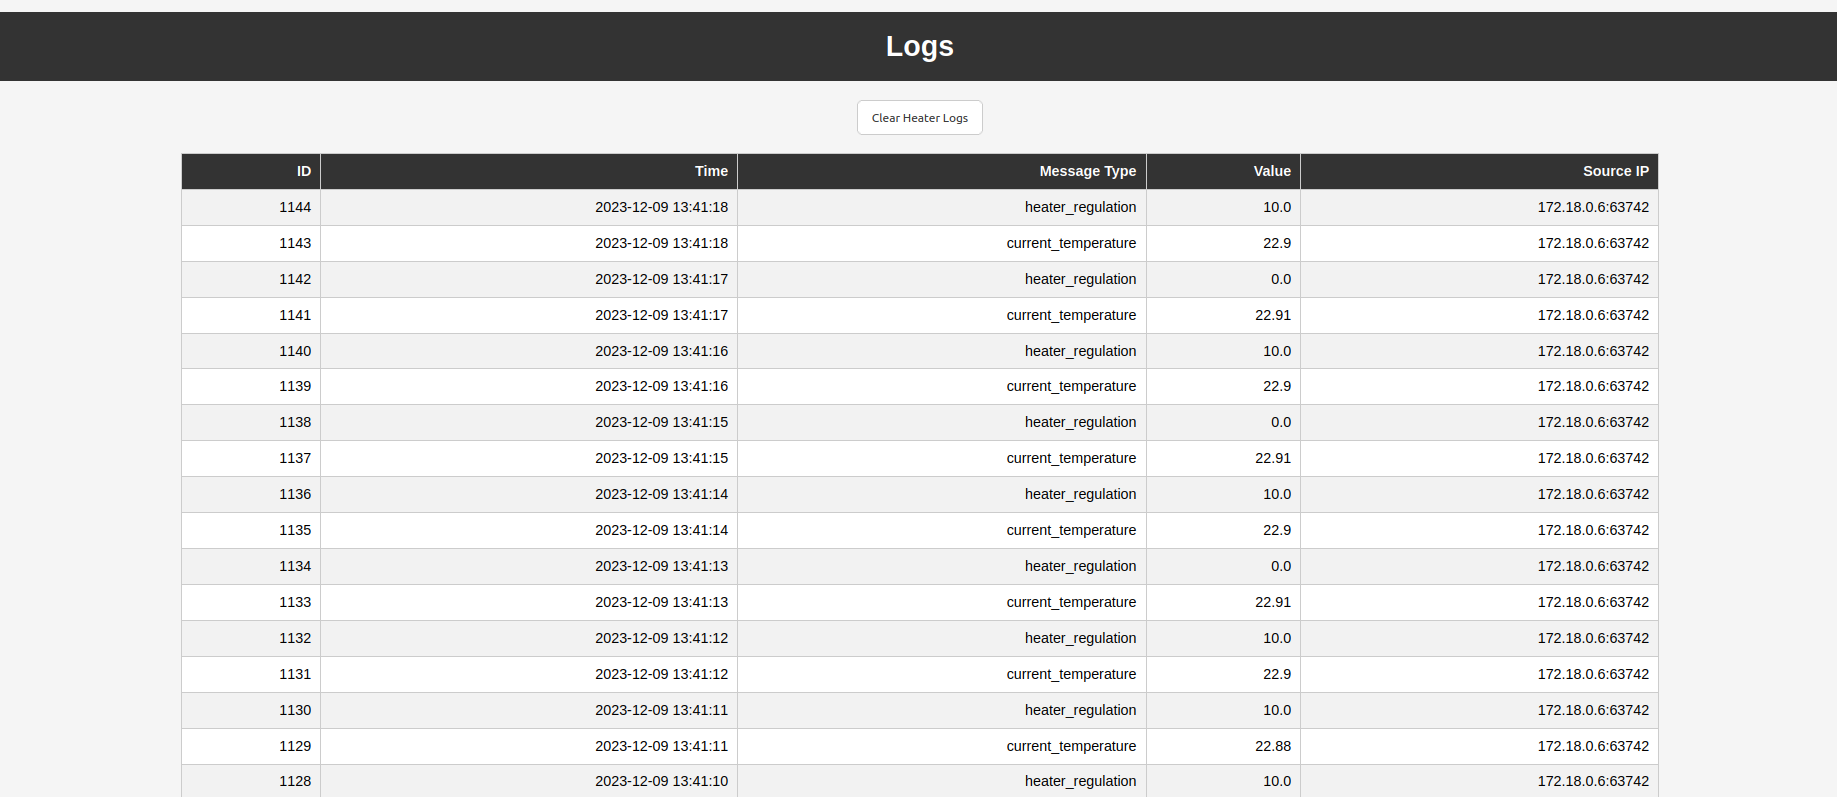
\includegraphics[width=0.8\linewidth]{graphics/screenshots/web-gui-logs.png}
                \caption{Zrzut ekranu przedstawiający panel Web GUI przeznaczony do obserwacji logów systemu.}
                \label{fig:web-gui-logs}
            \end{figure}

    \subsection{Symulacja}
    W wyniku założenia o symulacyjnym charakterze prototypowego systemu tj. braku uwzględnienia rzeczywistych czujników oraz układów regulacyjnych zaimplementowano ekosystem, który stanowi pewne przybliżenie środowiska, w którym mógłby operować system. 

    W układach HEATER oraz DIMMER zasymulowano zmiany temperatury, oraz natężenia oświetlenia z wykorzystaniem licznika systemowego. Wraz z przerwaniem licznika, które dla HEATER następuje co 100ms, natomiast dla DIMMER co 200ms, aktualna temperatura oraz aktualne natężenie oświetlenia zastępowane są nową temperaturą, oraz nowym natężeniem oświetlenia. 

    Temperatura środowiska w układzie HEATER opisana jest następującym wzorem:
        \[nowa\_temperatura = aktualna\_temperatura + a\cdot parametr\_regulacji + b\]
    Gdzie:
    \begin{itemize}
        \item \textit{a = 0,00025},
        \item \textit{b = -5a}. 
    \end{itemize}

    Natomiast zmiany natężenia środowiska w układzie DIMMER opisuje funkcja:
    \[nowe\_no= aktualne\_no + a\cdot parametr\_regulacji\]
    Gdzie:
    \begin{itemize}
        \item \textit{nowe\_no} - nowe natężenie oświetlenia,
        \item \textit{aktualne\_no} - aktualne natężenie oświetlenia,
        \item \textit{a = 0,00025}
    \end{itemize}

    Wprowadzony parametr b we wzorze na chwilową temperaturę ekosystemu w układzie HEATER pozwala na zasymulowanie powolnego spadku temperatury. Środowisko wdrożone w Układzie DIMMER można przyjąć za izolowane, ponieważ nie uwzględnia żadnych zewnętrznych źródeł światła.
    Parametry a oraz b dla obydwu układów, zostały wyznaczone empirycznie, aby zagwarantować możliwość zaobserwowania zmian wynikających z poprawnego działania systemu.
    
    \subsection{Zasada działania}
    \label{subsec:system-behaviour}

    Celem niniejszej podsekcji jest opisanie zasady działania wdrożonego systemu automatyki domowej, poprzez przegląd logiki aplikacji oraz przepływu informacji między komponentami.
    
    Zachowanie systemu można podzielić na 3 fazy:
    \begin{itemize}
        \item Fazę ustalania parametrów systemu - użytkownik nadaje systemowi stan, do którego mają dążyć układy regulacyjne.
        \item Fazę pomiarów - układ pomiarowy przesyła aktualny stan parametru System Controllerowi.
        \item Fazę regulacji - układ regulacji odpytuje System Controller o nową wartość parametru regulacji w celu utrzymania parametrów środowiska dążących do zadanego przez użytkownika stanu.
    \end{itemize}

    Ustalanie parametrów systemu odbywa się asynchronicznie przez użytkownika, natomiast regulacja oraz pomiar wykonywane są periodycznie z okresem 1s.

        \subsubsection{Ustalanie parametrów systemu}

            Na Rysunku \ref{fig:seq-user-webgui-db} zilustrowano przepływ wiadomości między komponentami systemu w fazie ustalania parametrów systemu.

            \begin{figure}[H]
                \centering
                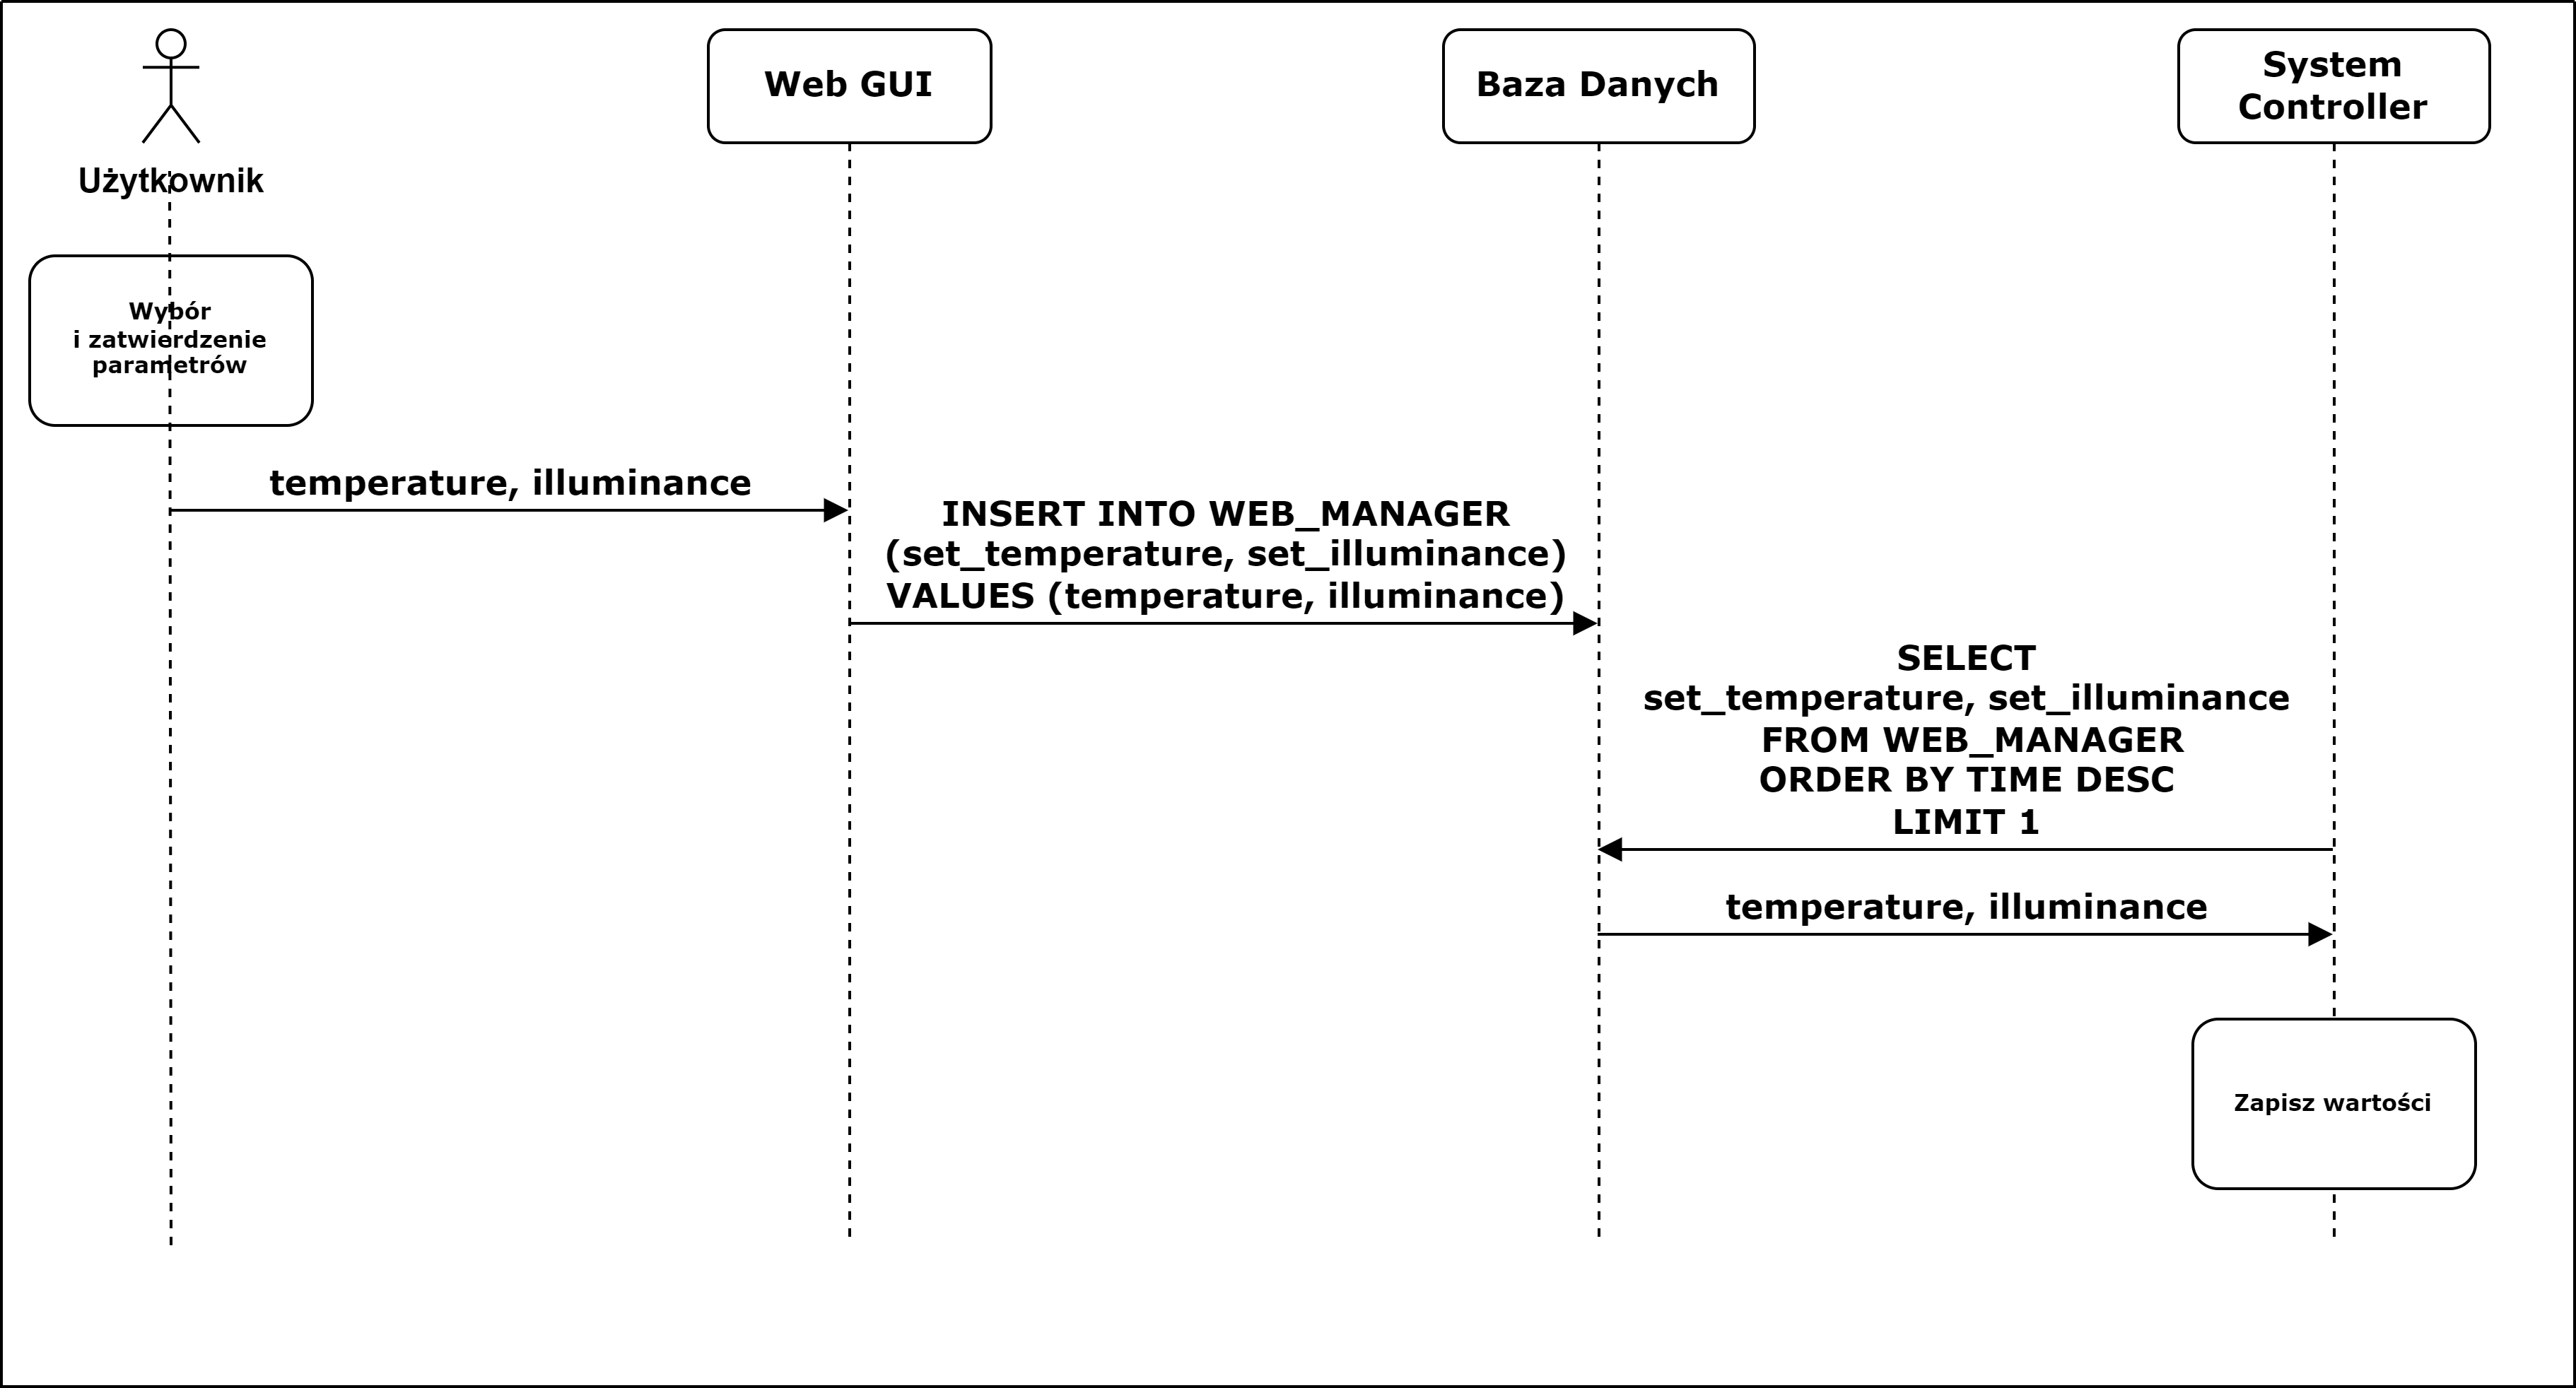
\includegraphics[width=0.8\linewidth]{graphics/sequence-diagrams/user-webgui-db-diagram.png}
                \caption{Diagram sekwencji ustawiania parametrów systemu.}
                \label{fig:seq-user-webgui-db}
            \end{figure}

            Kolejnymi krokami procedury są:
            \begin{enumerate}
                \item Użytkownik korzystający z panelu Web GUI, służącego do ustawiania parametrów systemu, zobrazowanym na Rysunku \ref{fig:web-gui-set-parameters}, podaje i zatwierdza wartości.
                \item Wprowadzone wartości \textit{temperature} oraz \textit{illuminance} wstawiane są do tabeli WEB\_MANAGER Bazy Danych.
                \item System Controller cyklicznie odpytuje Bazę Danych o ostatnio zaktualizowane wartości temperatury i natężenia oświetlenia.
                \item Po uzyskaniu wartości \textit{temperature} oraz \textit{illuminance} System Controller zapisuje je w swoim programie.
            \end{enumerate}

        \subsubsection{Pomiar}

            Na Rysunku \ref{fig:seq-heater-measure} zilustrowano przepływ wiadomości między komponentami systemu w fazie pomiaru temperatury.

            \begin{figure}[H]
                \centering
                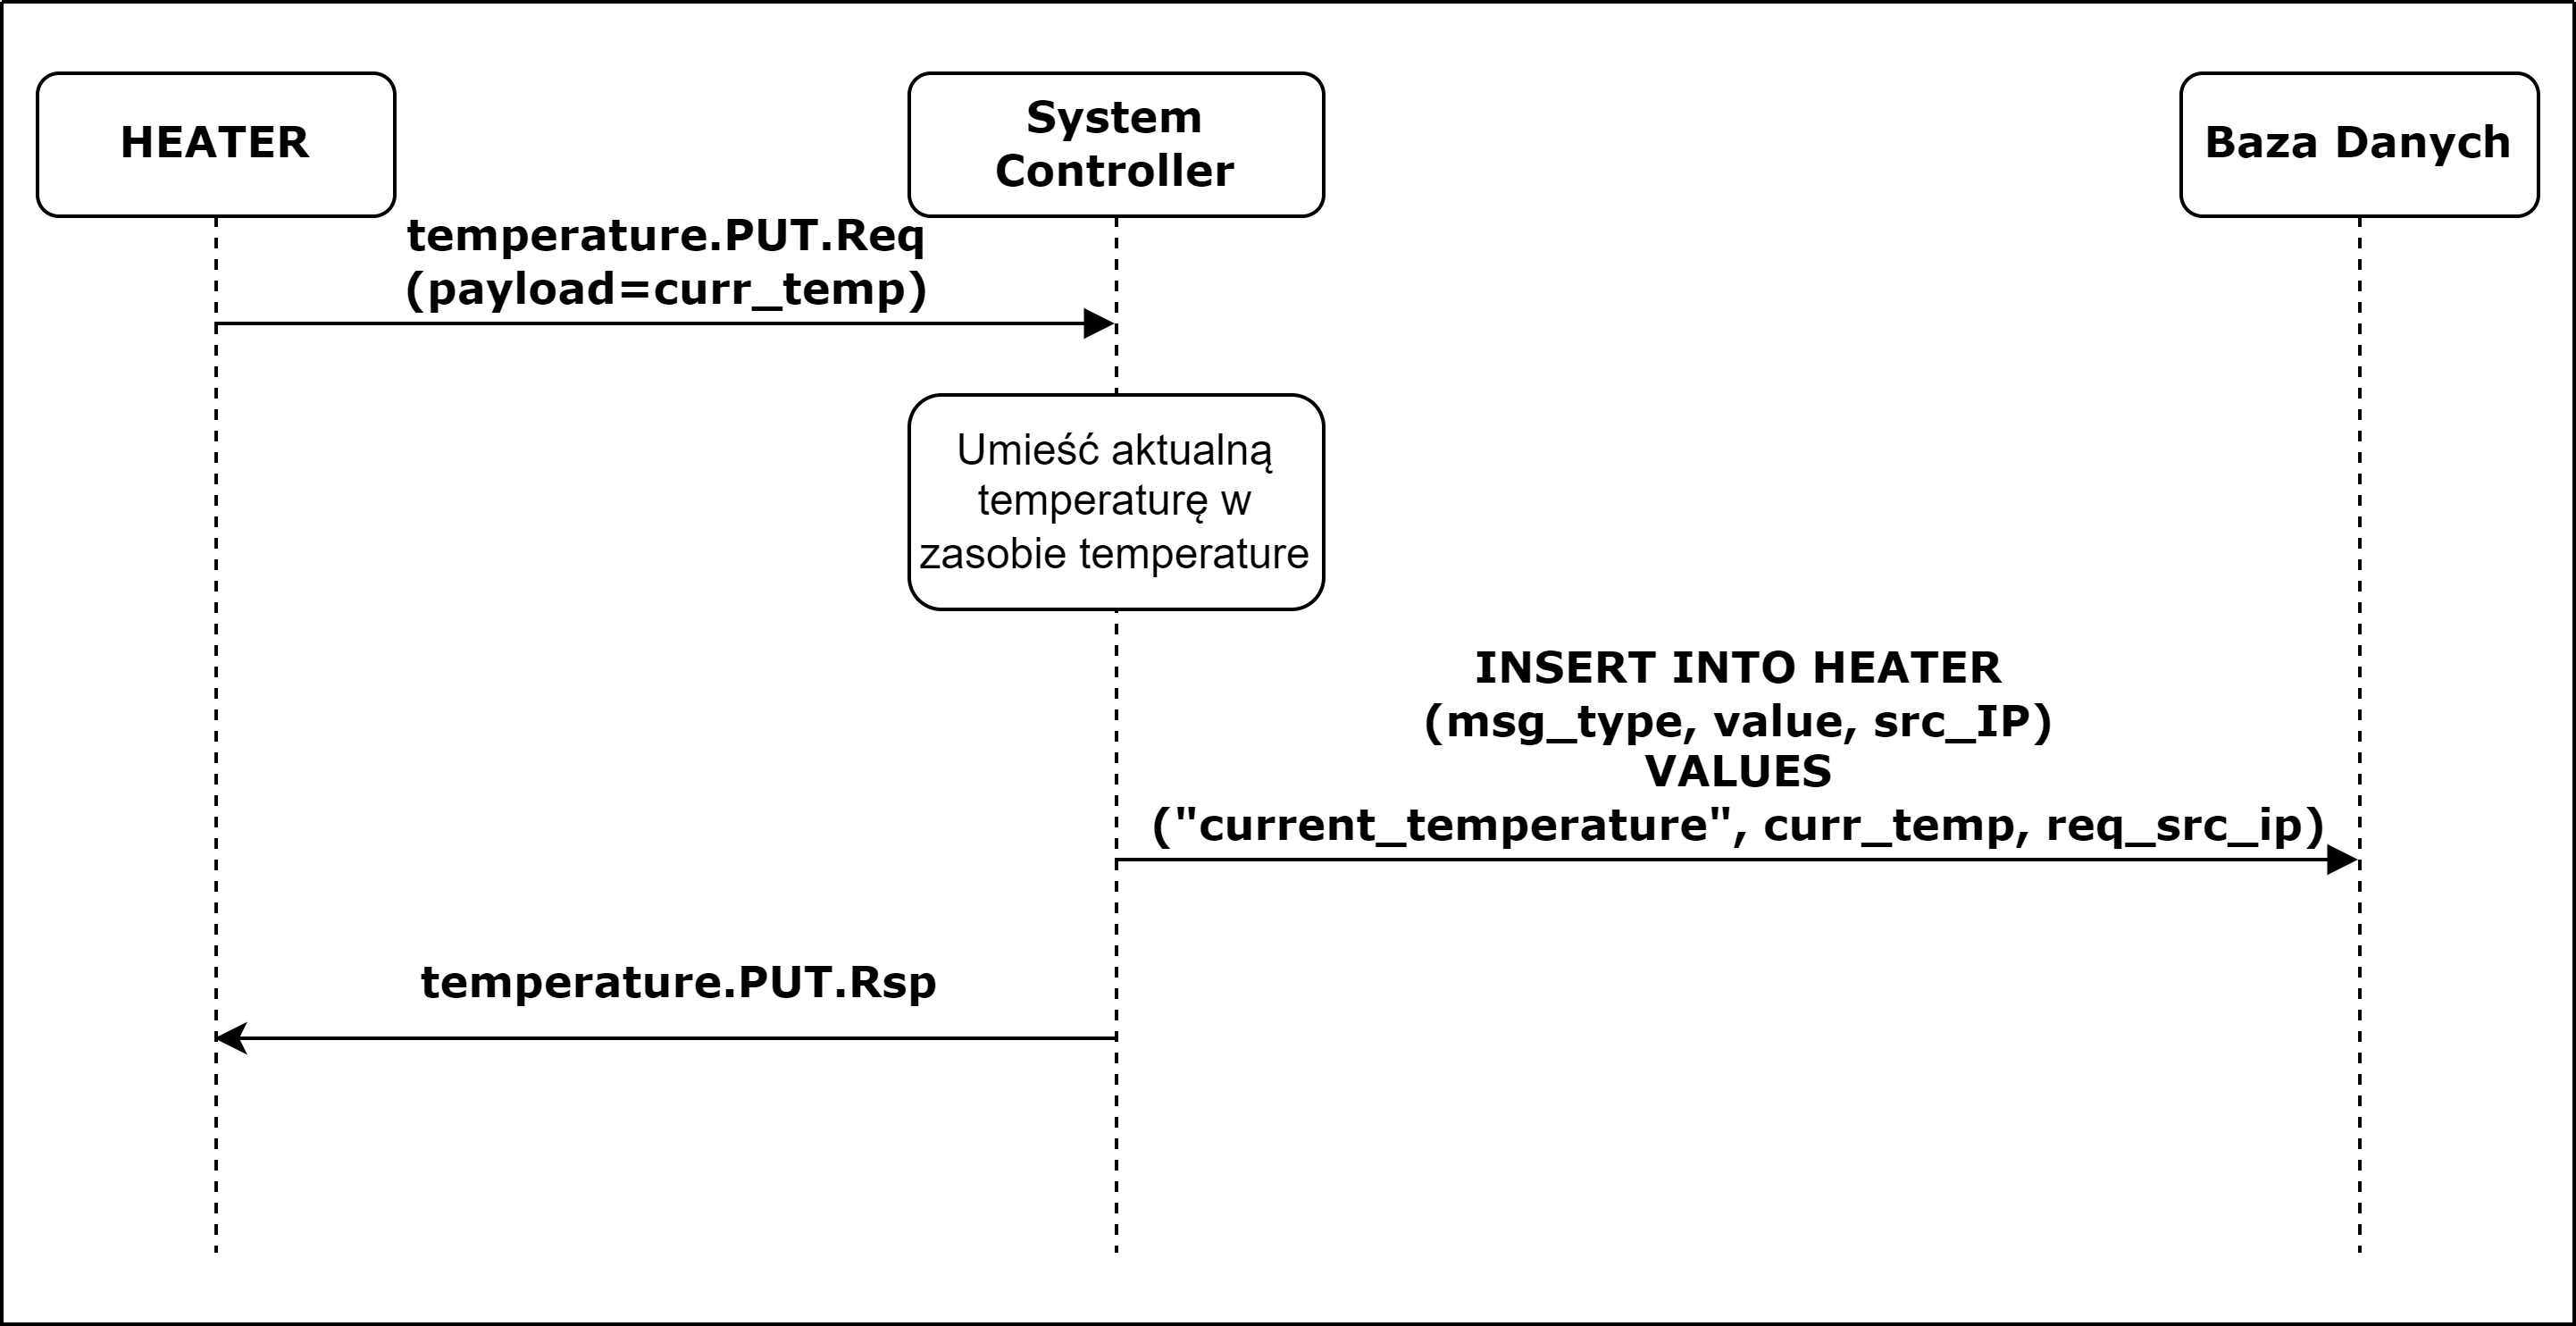
\includegraphics[width=0.8\linewidth]{graphics/sequence-diagrams/heater-measure-seq.png}
                \caption{Diagram sekwencji pomiaru temperatury.}
                \label{fig:seq-heater-measure}
            \end{figure}

            Kolejnymi krokami pomiaru temperatury w fazie pomiaru są:
            \begin{enumerate}
                \item Urządzenie HEATER wysyła zapytanie do System Controllera o umieszczenie aktualnej temperatury \textit{curr\_temp} w zasobie \textit{temperature}.
                \item System Controller umieszcza otrzymaną wartość \textit{curr\_temp} w zasobach serwera.
                \item System Controller loguje informację o przetworzonym zapytaniu, umieszczając otrzymaną wartość temperatury w tabeli HEATER Bazy Danych.
                \item System Controller w ramach potwierdzenia otrzymania zapytania odpowiada układowi HEATER.
            \end{enumerate}

            Na Rysunku \ref{fig:seq-dimmer-measure} zilustrowano przepływ wiadomości między komponentami systemu w fazie pomiaru natężenia oświetlenia.

            \begin{figure}[H]
                \centering
                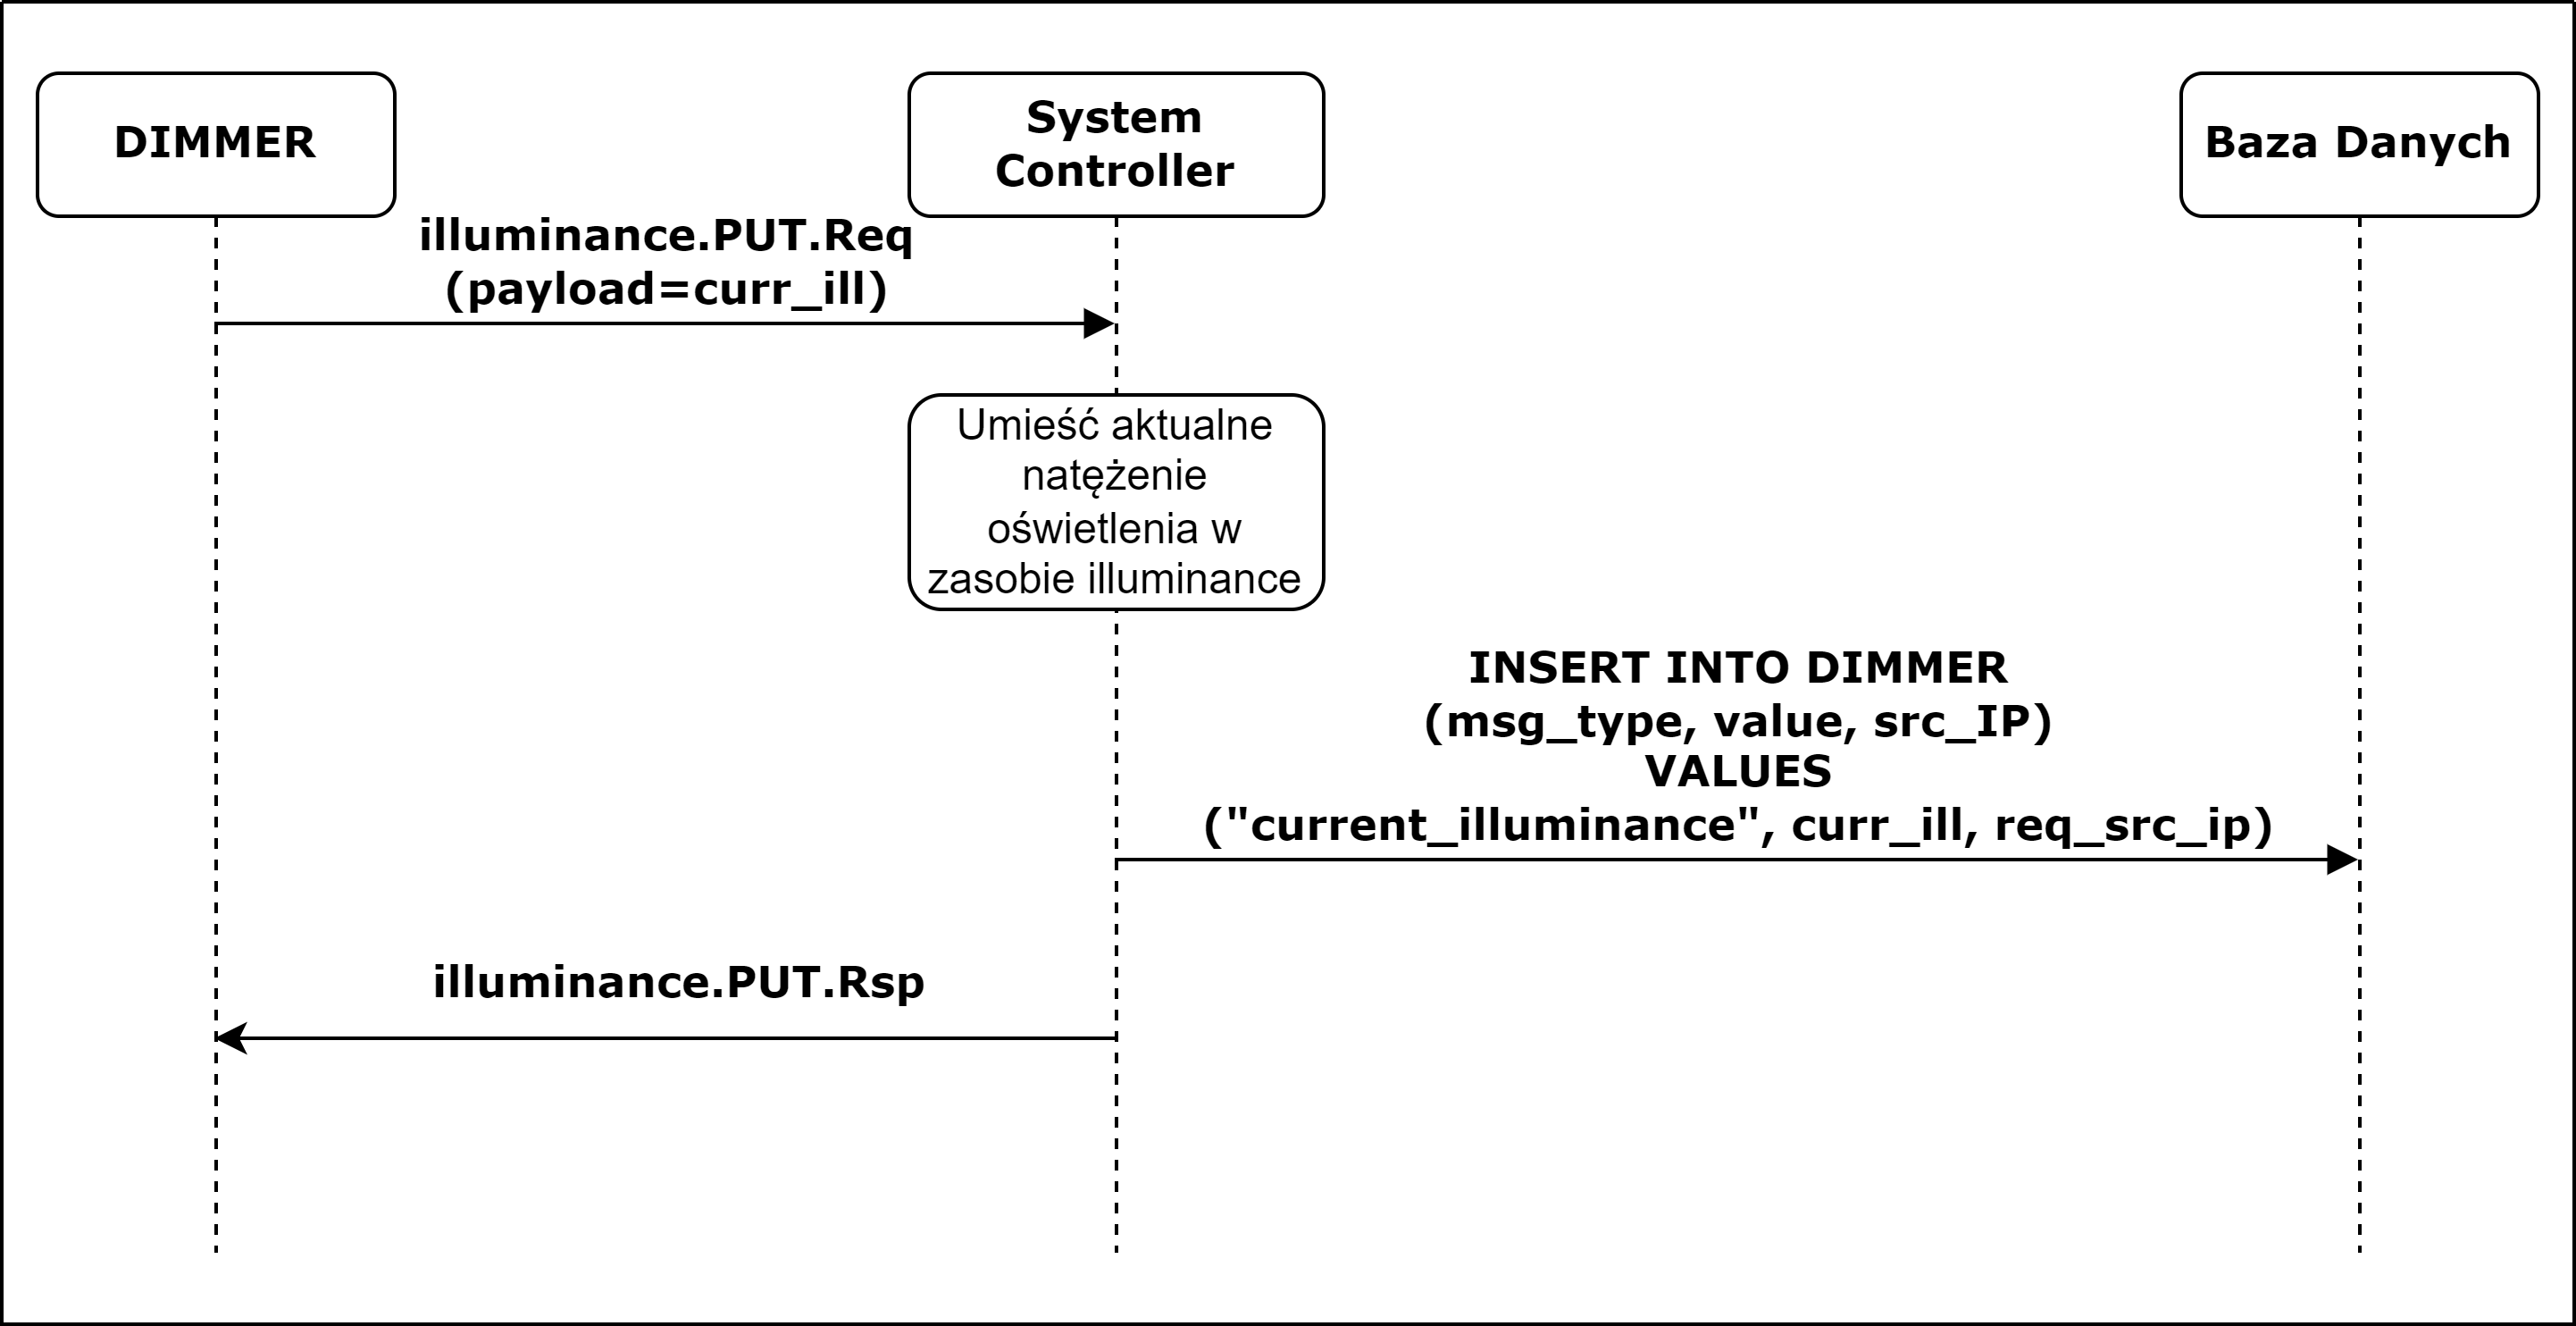
\includegraphics[width=0.8\linewidth]{graphics/sequence-diagrams/dimmer-measure-seq.png}
                \caption{Diagram sekwencji pomiaru natężenia oświetlenia.}
                \label{fig:seq-dimmer-measure}
            \end{figure}

            Kolejnymi krokami pomiaru natężenia oświetlenia w fazie pomiaru są:
            \begin{enumerate}
                \item Urządzenie DIMMER wysyła zapytanie do System Controllera o umieszczenie aktualnego natężenia oświetlenia \textit{curr\_ill} w zasobie \textit{illuminance}.
                \item System Controller umieszcza otrzymaną wartość natężenia oświetlenia \textit{curr\_ill} w zasobach serwera.
                \item System Controller loguje informację o przetworzonym zapytaniu, umieszczając otrzymaną wartość natężenia oświetlenia w tabeli DIMMER Bazy Danych.
                \item System Controller w ramach potwierdzenia otrzymania zapytania odpowiada układowy HEATER.
            \end{enumerate}


        \subsubsection{Regulacja}

            Na Rysunku \ref{fig:seq-heater-regulate} zilustrowano przepływ wiadomości między komponentami systemu w fazie regulacji temperatury.

            \begin{figure}[H]
                \centering
                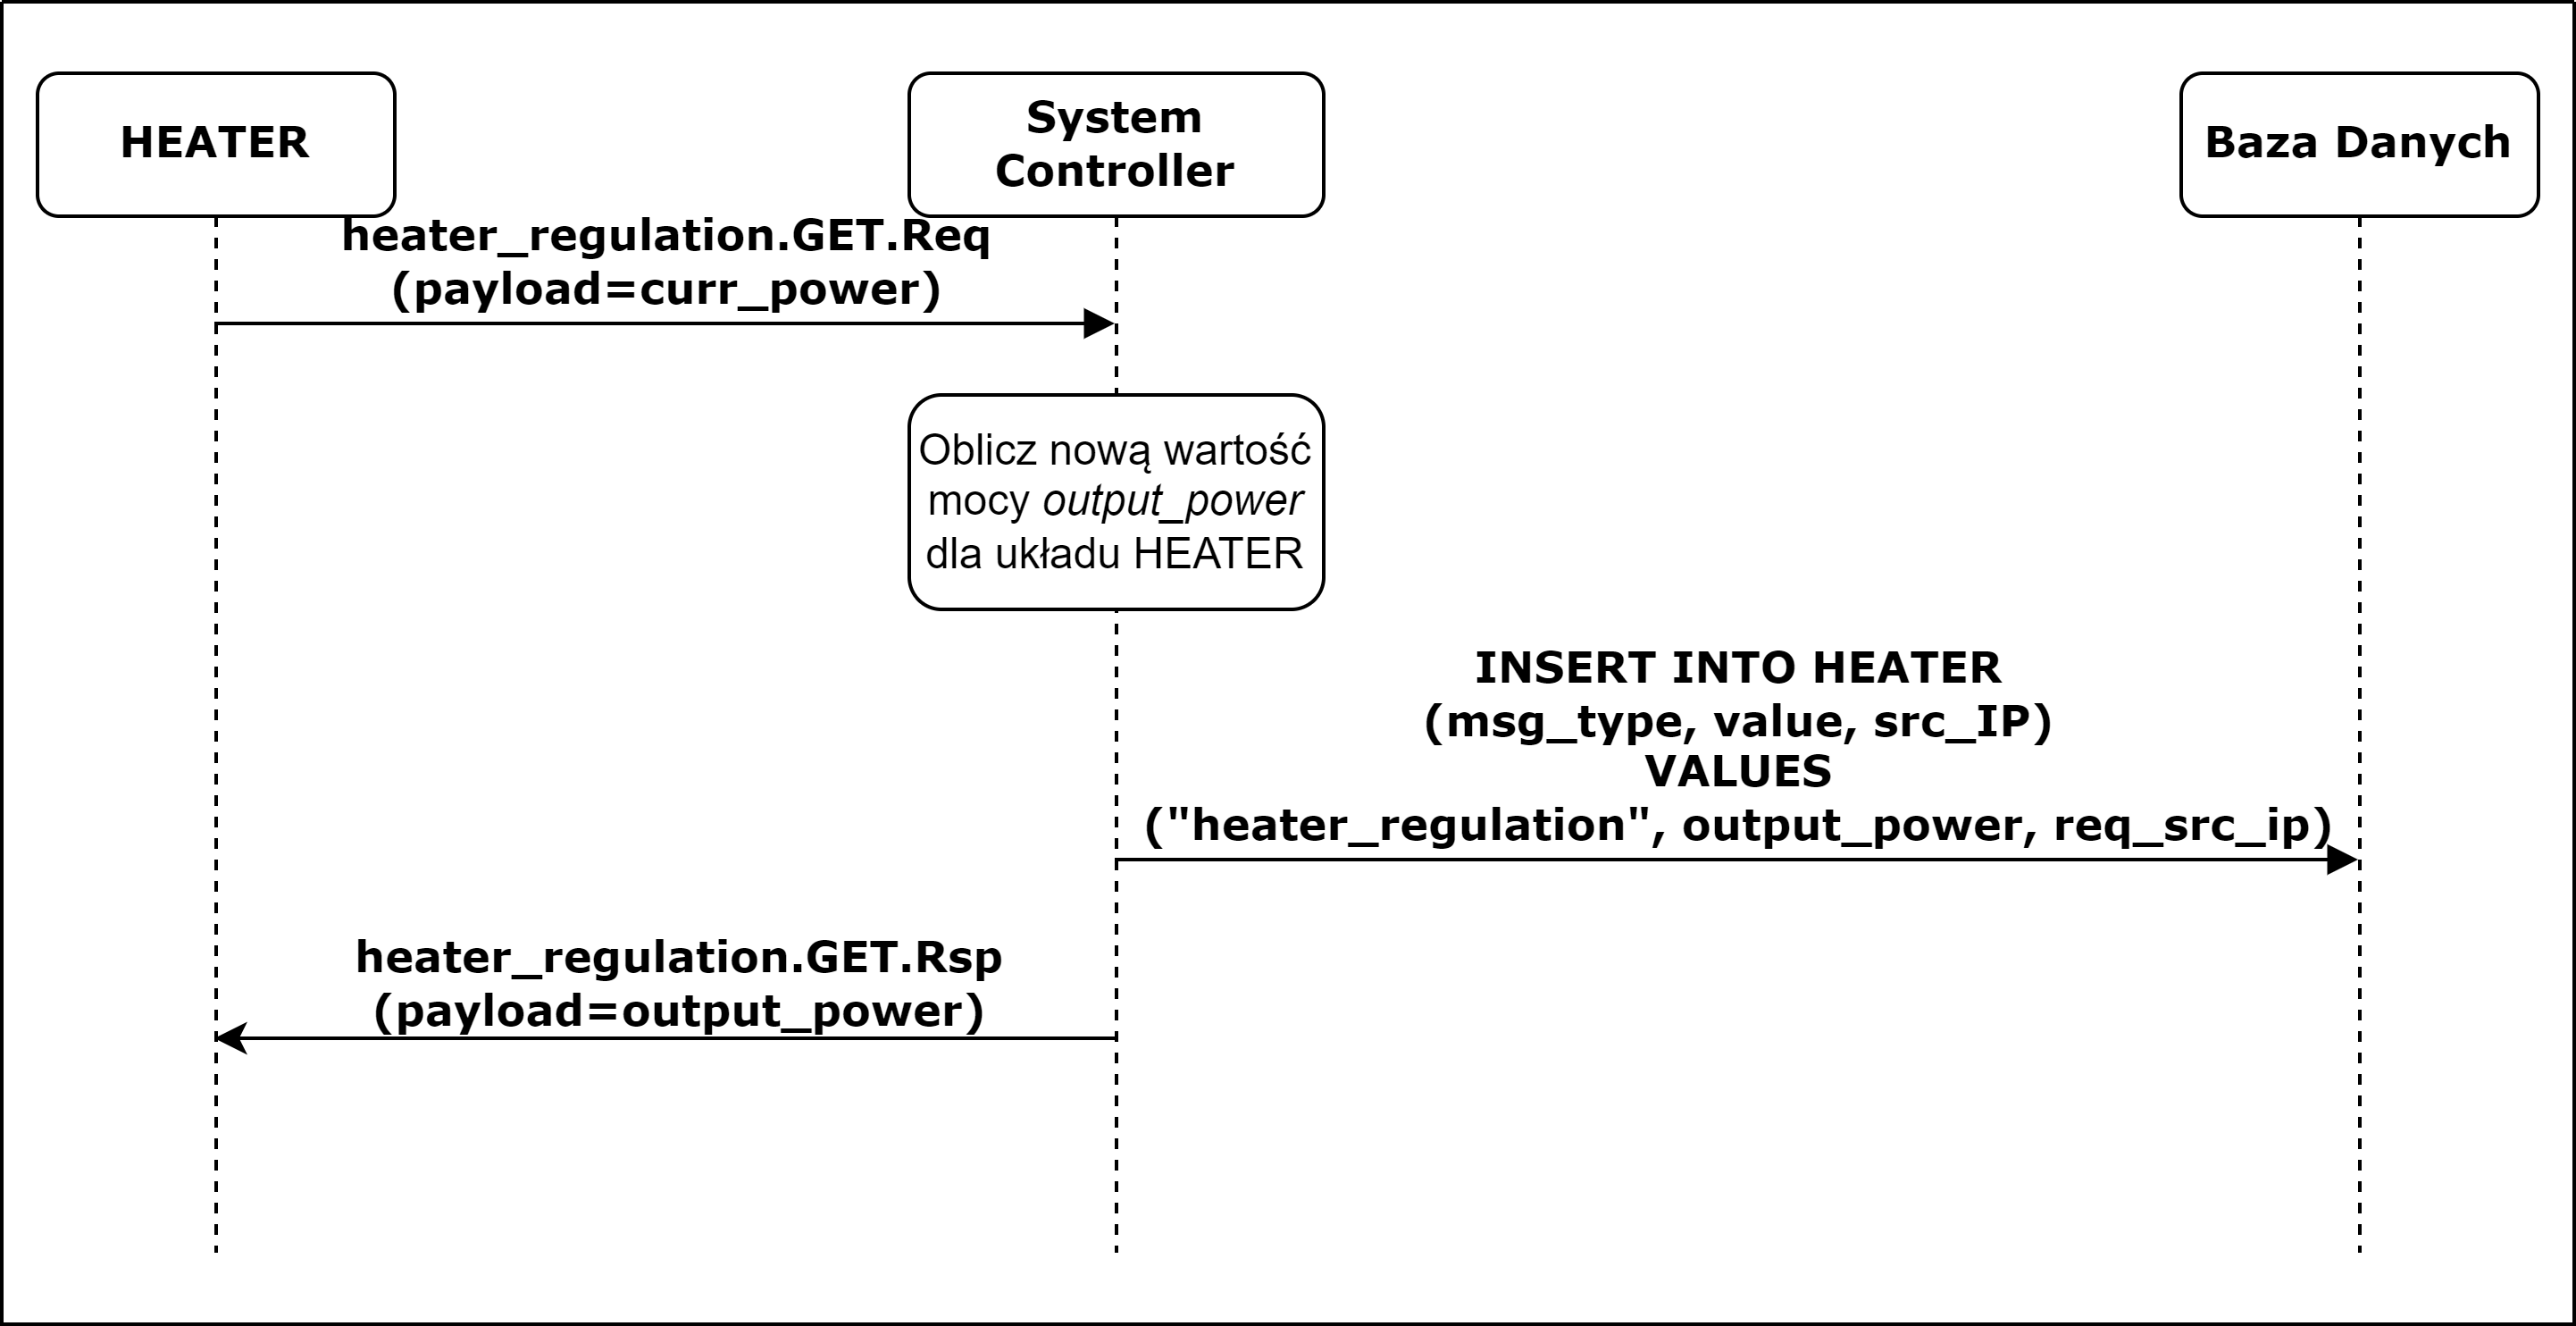
\includegraphics[width=0.8\linewidth]{graphics/sequence-diagrams/heater-regulate-seq.png}
                \caption{Diagram sekwencji regulacji temperatury.}
                \label{fig:seq-heater-regulate}
            \end{figure}

            \begin{figure}[H]
                \centering
                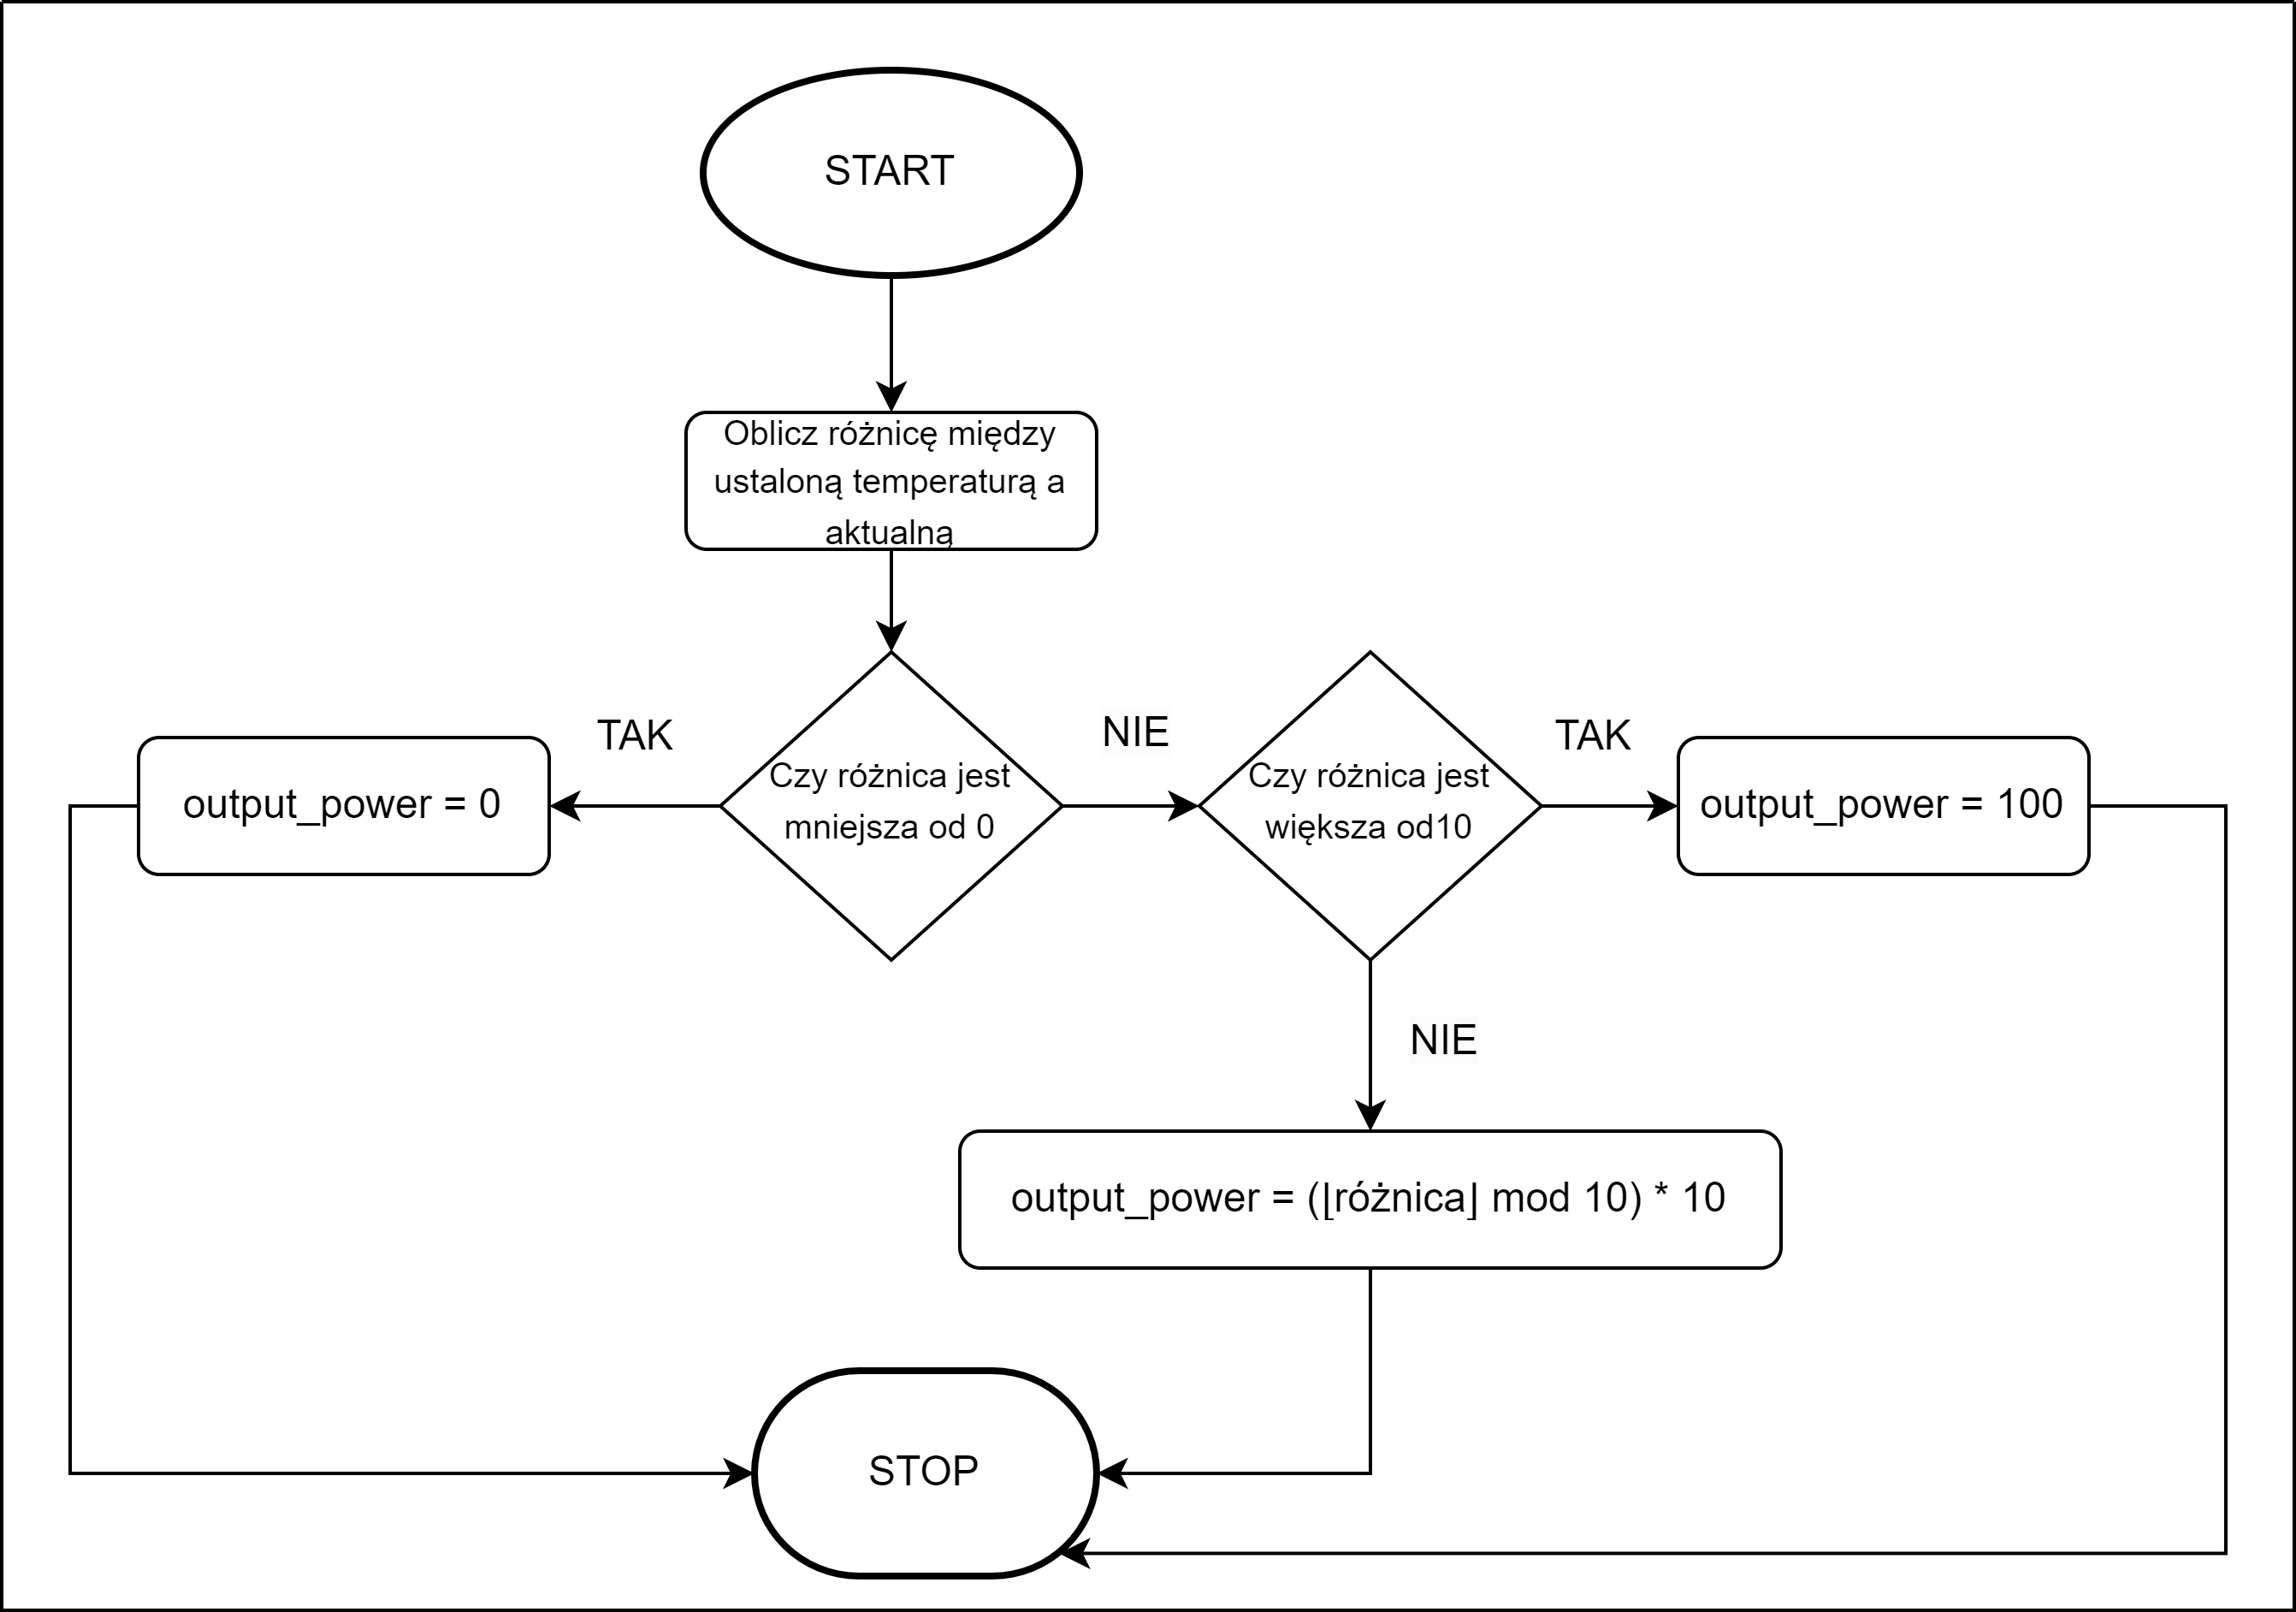
\includegraphics[width=0.8\linewidth]{graphics/heater-block-diagram.png}
                \caption{Algorytm obliczania parametru mocy dla układu HEATER.}
                \label{fig:seq-heater-algo}
            \end{figure}

            Kolejnymi krokami regulacji temperatury w fazie regulacji są:
            \begin{enumerate}
                \item Urządzenie HEATER wysyła zapytanie do System Controllera o otrzymanie nowego parametru regulacji w zasobie \textit{heater\_regulation}, w którym umieszcza aktualną wartość parametru regulacji \textit{curr\_power}.
                \item System Controller oblicza nową wartość \textit{output\_power} na podstawie aktualnej temperatury, umieszczonej w zasobie \textit{temperature} oraz aktualnej wartości parametru regulacji \textit{curr\_power}, zgodnie z algorytmem przedstawionym na Rysunku \ref{fig:seq-heater-algo}.
                \item System Controller loguje informację o przetworzonym zapytaniu, umieszczając obliczoną wartość \textit{output\_power} w tabeli HEATER Bazy Danych.
                \item System Controller odpowiada układowy HEATER, dostarczając nową wartość parametru regulacji \textit{output\_power}.
            \end{enumerate}

            Na Rysunku \ref{fig:seq-dimmer-regulate} zilustrowano przepływ wiadomości między komponentami systemu w fazie regulacji natężenia oświetlenia.

            \begin{figure}[H]
                \centering
                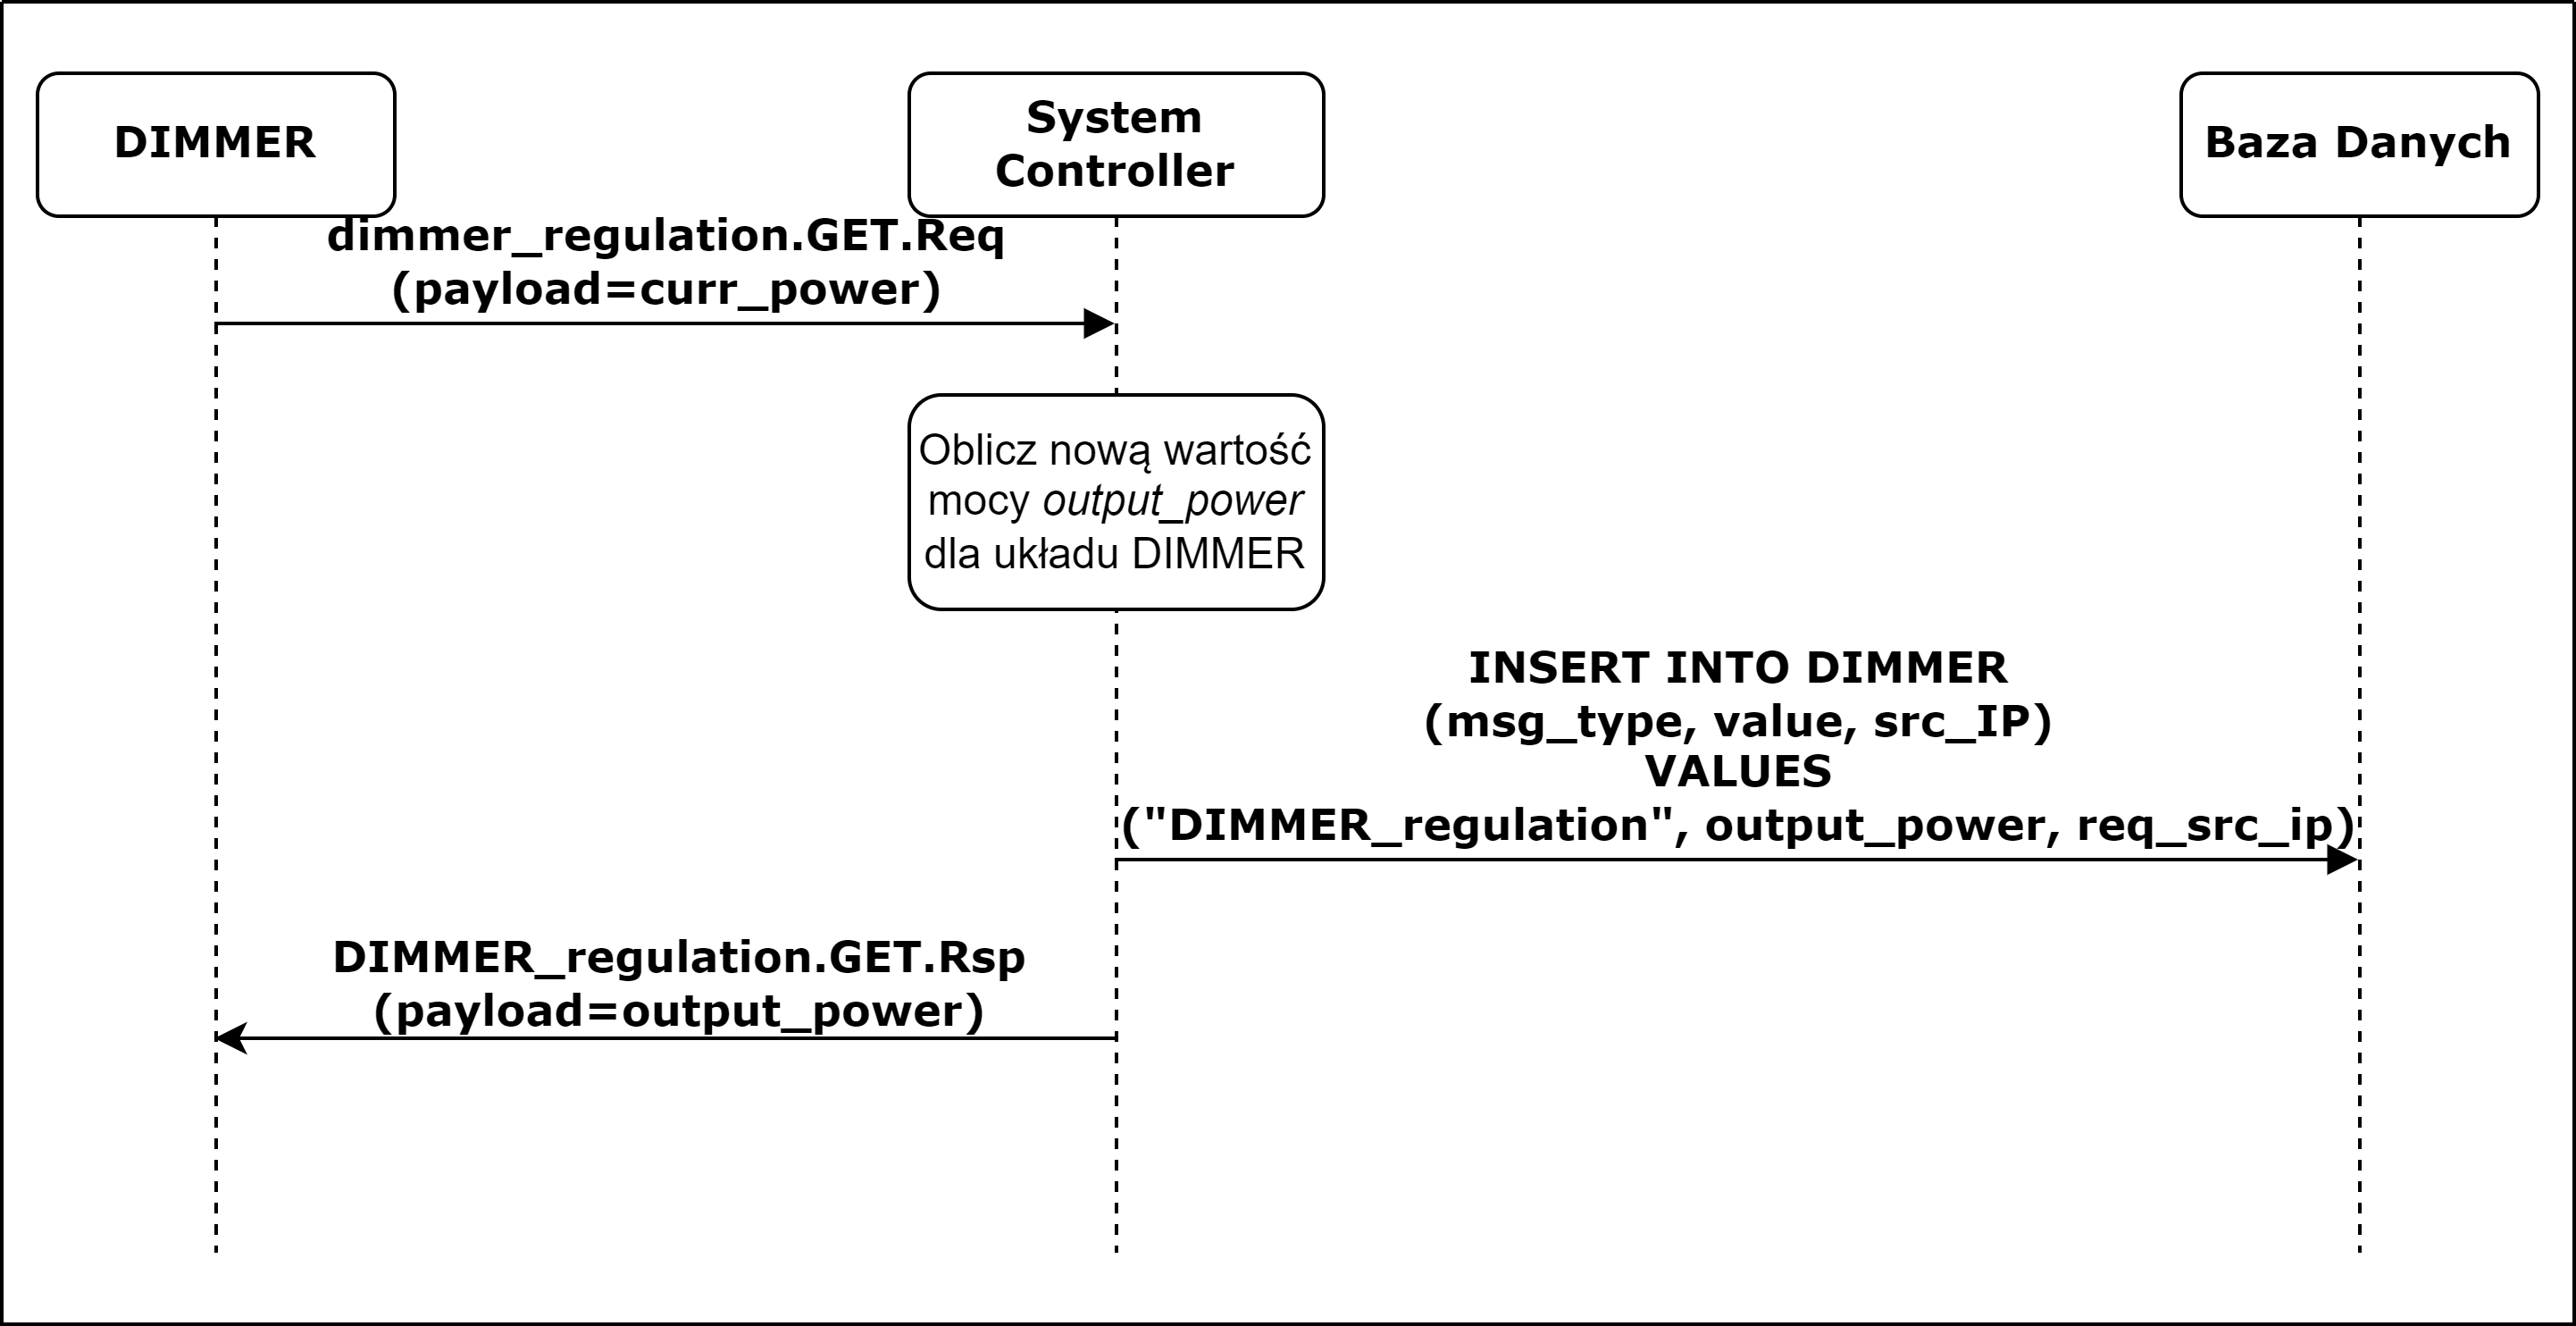
\includegraphics[width=0.8\linewidth]{graphics/sequence-diagrams/dimmer-regulate-seq.png}
                \caption{Diagram sekwencji regulacji natężenia oświetlenia.}
                \label{fig:seq-dimmer-regulate}
            \end{figure}

            \begin{figure}[H]
                \centering
                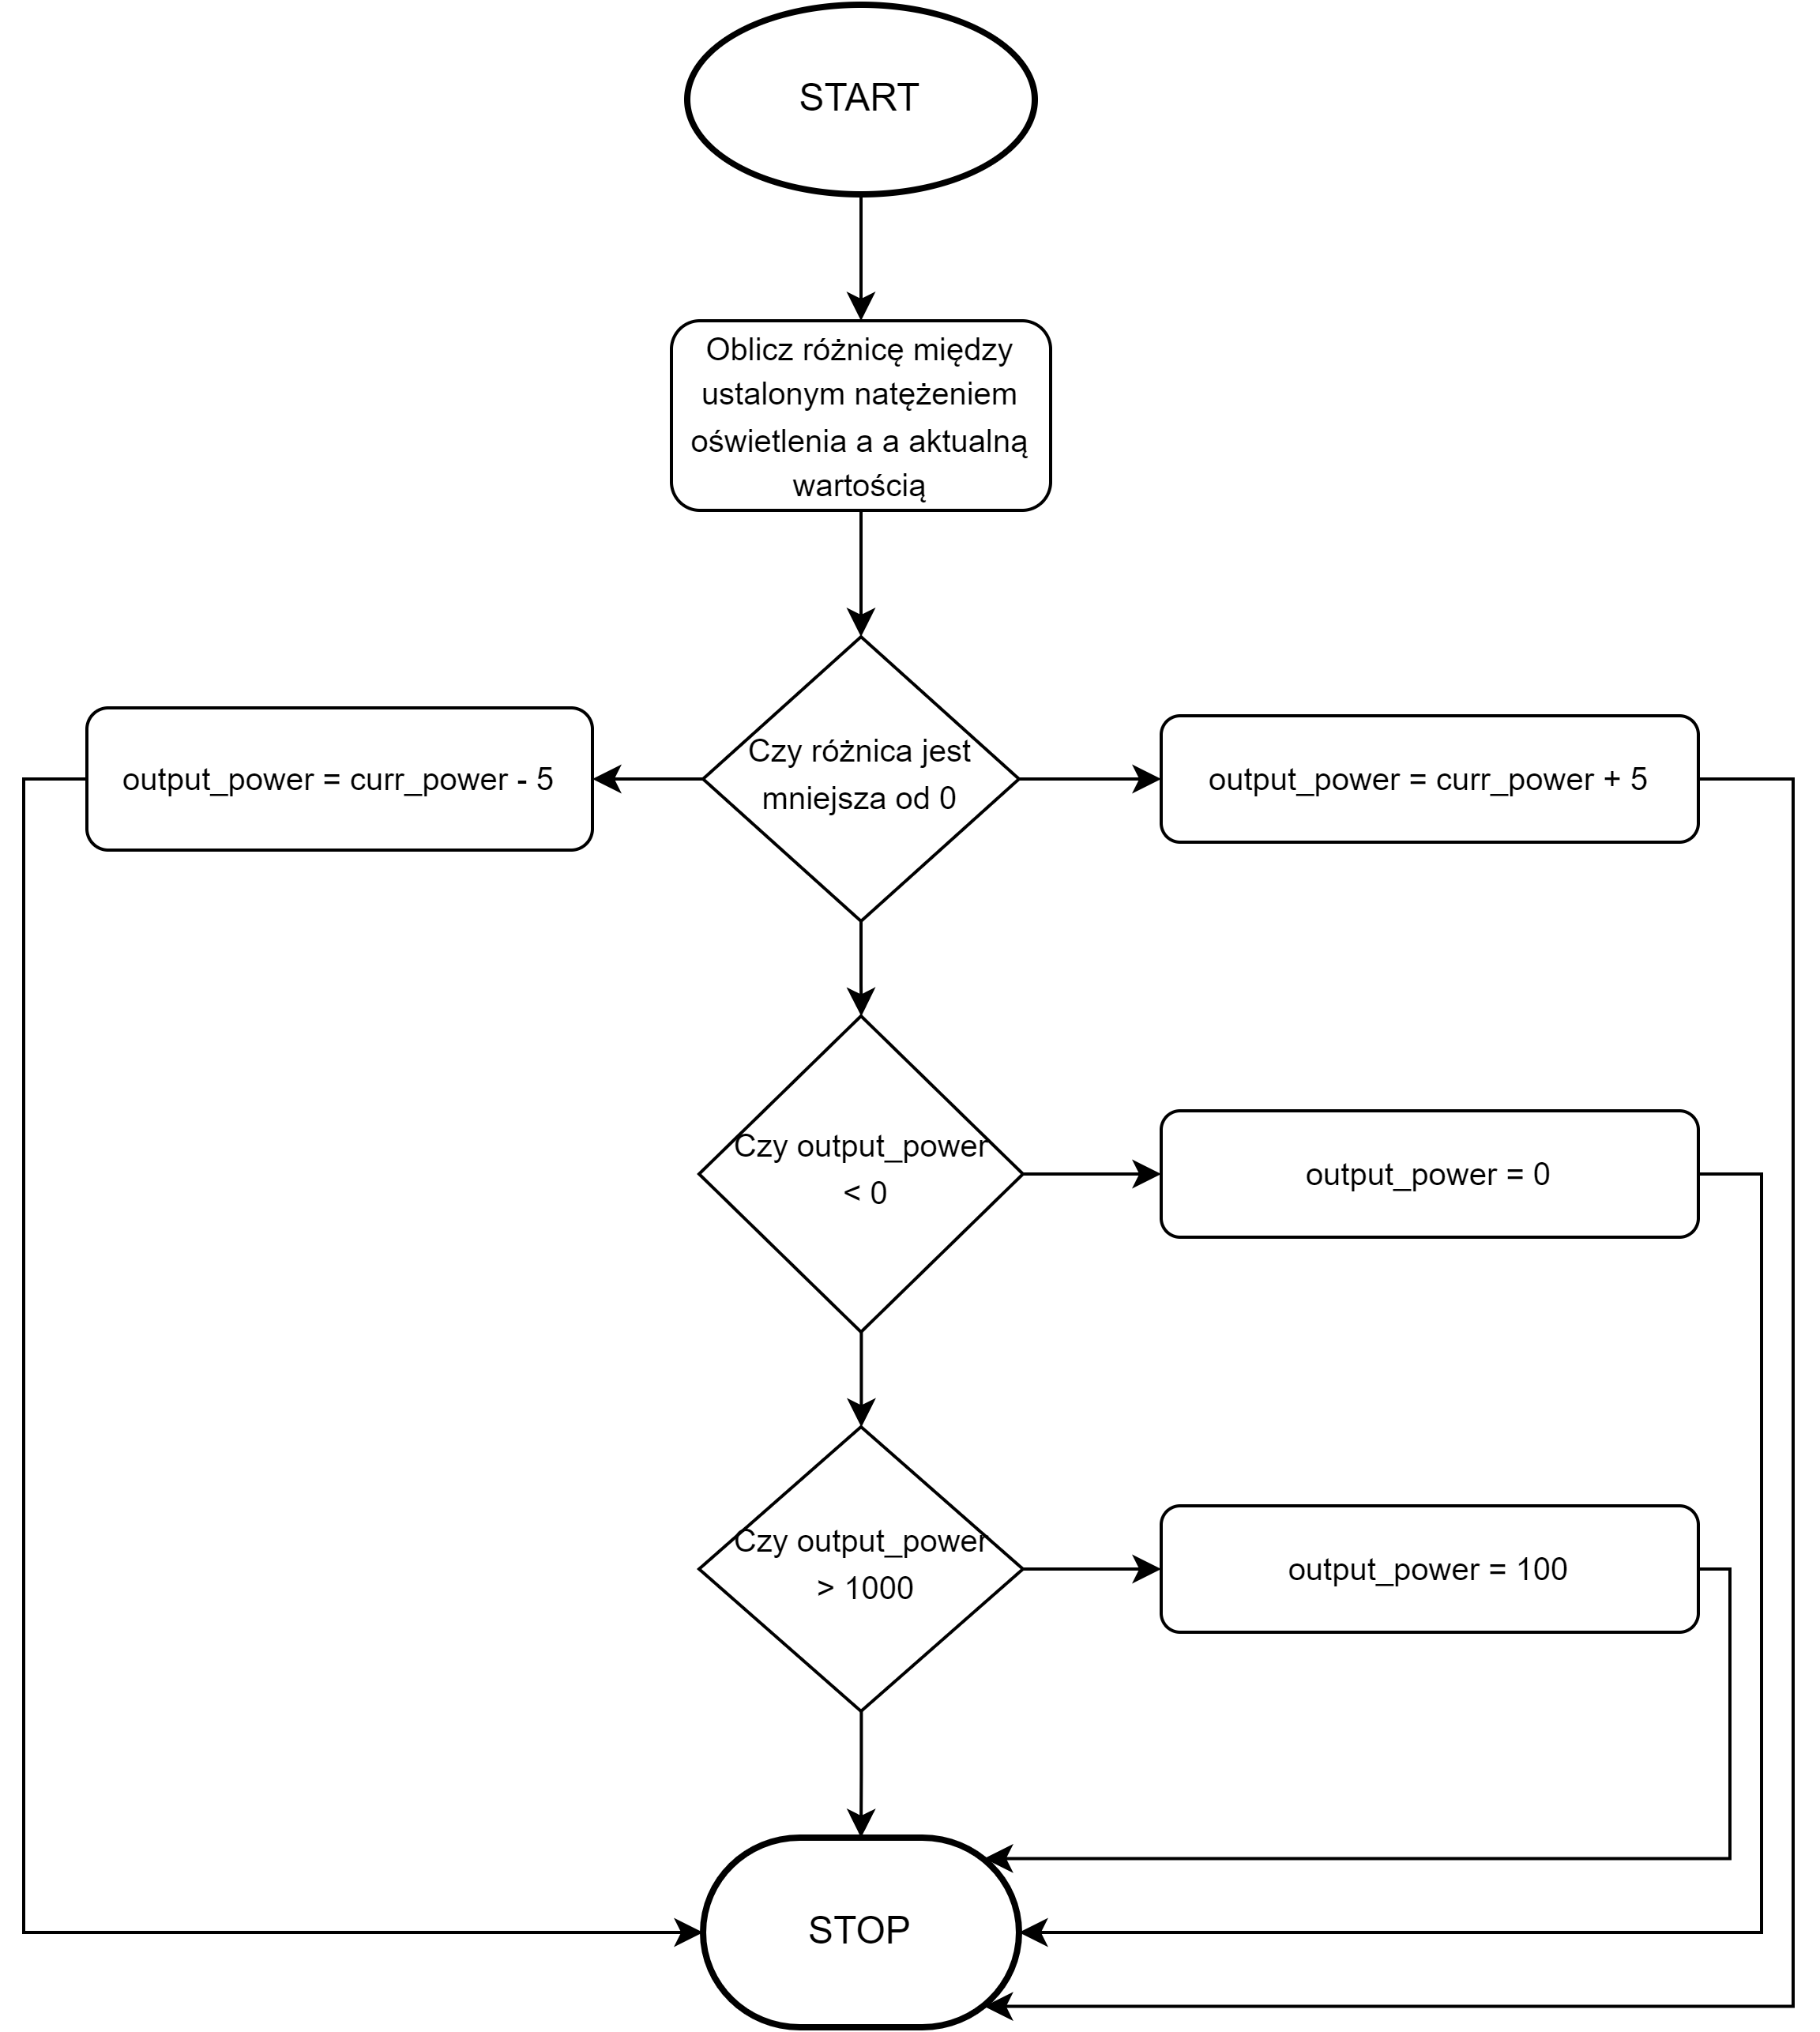
\includegraphics[width=0.8\linewidth]{graphics/dimmer-block-diagram.png}
                \caption{Algorytm obliczania parametru regulacji dla układu DIMMER.}
                \label{fig:seq-dimmer-algo}
            \end{figure}

            Kolejnymi krokami regulacji natężenia oświetlenia w fazie regulacji są:
            \begin{enumerate}
                \item Urządzenie DIMMER wysyła zapytanie do System Controllera o otrzymanie nowego parametru regulacji w zasobie \textit{dimmer\_regulation}, w którym umieszcza aktualną wartość parametru regulacji \textit{curr\_power}.
                \item System Controller oblicza nową wartość \textit{output\_power} na podstawie wartości aktualnego natężenia oświetlenia, umieszczonego w zasobie \textit{illuminance} oraz poprzedniej wartości parametru regulacji \textit{curr\_power}, zgodnie z algorytmem przedstawionym na Rysunku \ref{fig:seq-dimmer-algo}.
                \item System Controller loguje informację o przetworzonym zapytaniu, umieszczając obliczoną wartość \textit{output\_power} w tabeli DIMMER Bazy Danych.
                \item System Controller odpowiada układowy DIMMER, dostarczając nową wartość parametru regulacji \textit{output\_power}.
            \end{enumerate}

            W związku z charakterem pracy, w której nacisk implementacji projektu został położony na aspekty komunikacji, dobrane algorytmy przedstawione na Rysunku \ref{fig:seq-heater-algo} oraz Rysunku \ref{fig:seq-dimmer-algo} pozwalają na zaprezentowanie działania prototypowego systemu, natomiast nie są optymalne. We wdrożonych algorytmach System Controllera brakuje histerezy, co w konsekwencji mogłoby spowodować skokowe zmiany obliczanego parametru regulacji przy niewielkich odchyleniach wartości temperatury oraz natężenie oświetlenia środowiska w stosunku do zadanego stanu. Opisane zachowanie mogłoby mieć wpływ na żywotność baterii urządzeń, które pracują jako regulator. Jednym z rozwiązań problemu mogłoby być zastosowanie w System Controllerze algorytmu opartego o PID (ang. \textit{Proportional-Integral-Derivative}).

\chapter{Uruchomienie i weryfikacja poprawności działania systemu}

Celem niniejszego rozdziału jest opisanie procesu uruchomienia systemu oraz weryfikacji poprawności działania, poprzez sprawdzenie połączeń między węzłami sieci Thread oraz zasady działania systemu, przedstawionych w podsekcji \ref{subsec:system-behaviour}.

\section{Uruchomienie}

Pierwszym krokiem w uruchomieniu systemu, jest utworzenie sieci Thread. Proces tworzenie topologii rozpoczęto od wystartowania aplikacji OTBR.

Podłączono zaprogramowaną platformę, jak omówiono w Podsekcji \ref{subsec:otbr-implementation}, do portu szeregowego urządzenia gospodarza, a następnie sprawdzono poprawność komunikacji między maszyną wirtualną a urządzeniem pracującym jako RCP. Ostatecznie uruchomiono kontener Docker, zawierający aplikację OTBR, wykorzystując przygotowany wcześniej skrypt \textit{my-run-otbr.sh} znajdujący się w repozytorium \cite{project-repo}. Upewniwszy się o poprawnym działaniu Rutera Brzegowego, rozpoczęto tworzenie sieci Thread.
    
Do konfiguracji sieci wykorzystano interfejs graficzny OTBR Web GUI, będący serwisem zapewnionym w ramach aplikacji OTBR. Zrzut ekrany przedstawiającego wymieniony interfejs graficzny, zaprezentowano na Rysunku \ref{fig:otbr-web-gui}.

\begin{figure}[H]
    \centering
    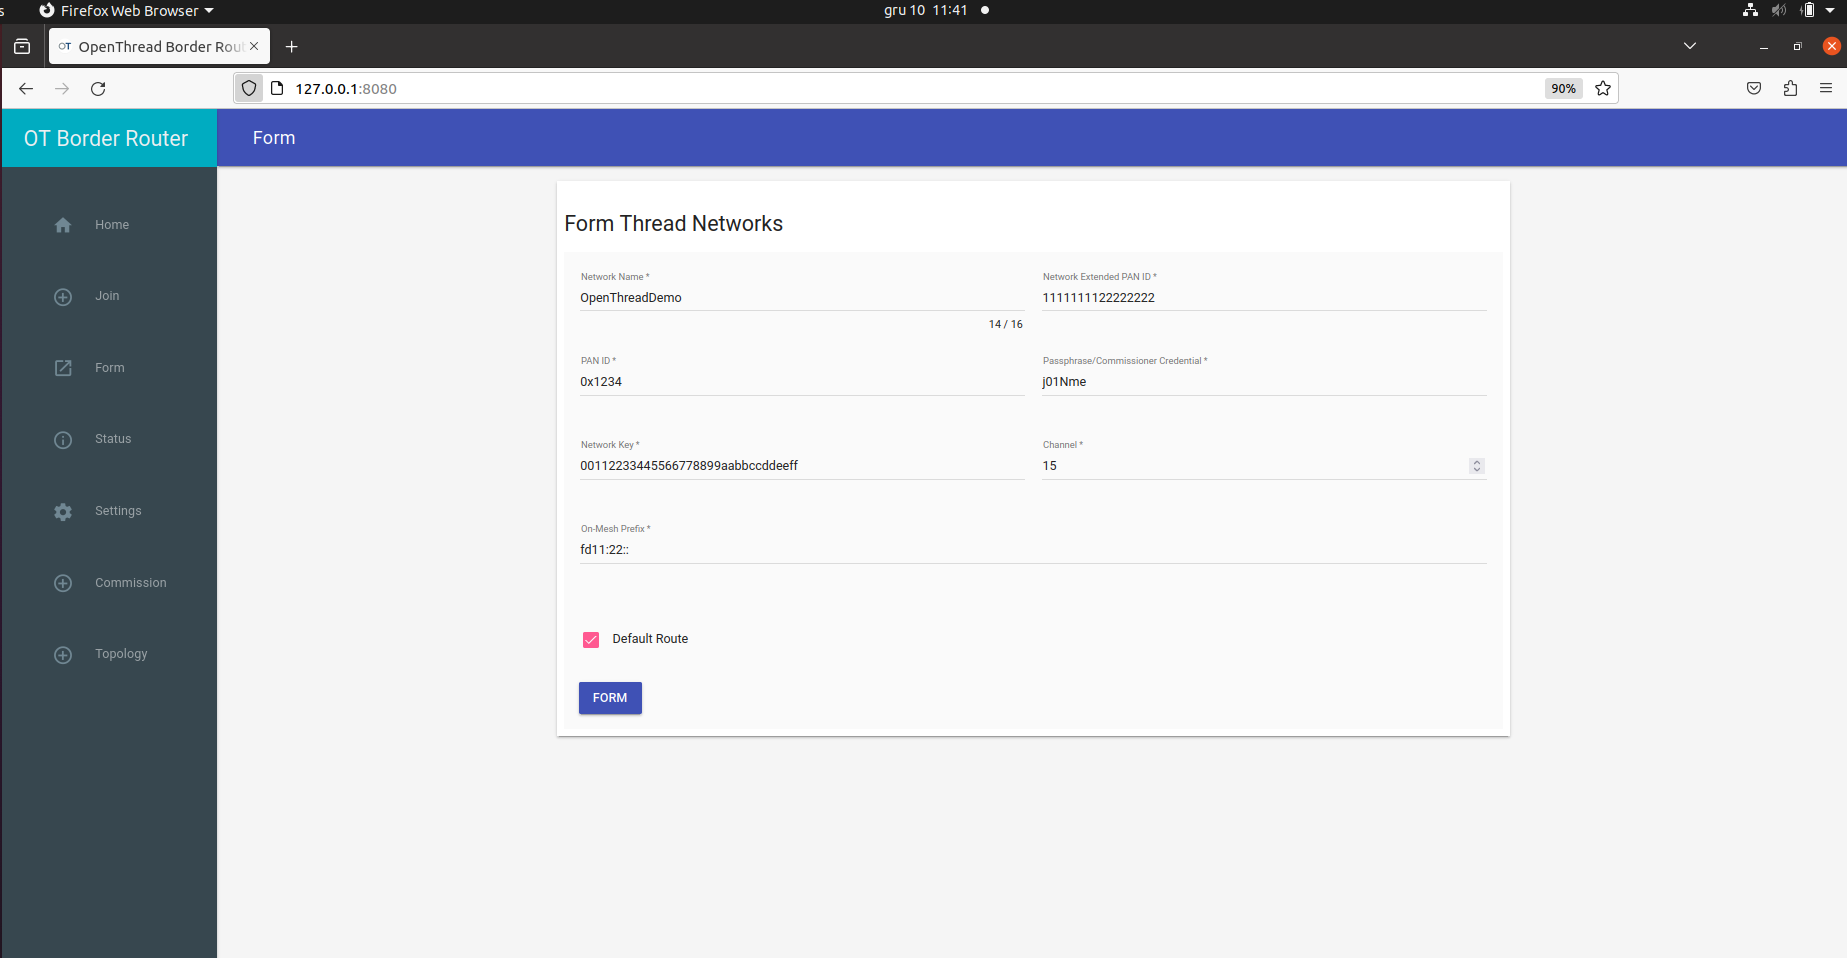
\includegraphics[width=0.8\linewidth]{graphics/screenshots/OTBR-web-gui.png}
    \caption{Zrzut ekranu interfejsu OTBR GUI z oknem do tworzenia sieci Thread.}
    \label{fig:otbr-web-gui}
\end{figure}

Wartości parametrów koniecznych do stworzenia sieci Thread, które opisano w Podsekcji \ref{subsec:network-forming}, przedstawiono w Tabeli \ref{tab:network-parameters}.

    \begin{table}[H]
    \centering
    \caption{Parametry sieci Thread.}
    \begin{tabular}{|l|l|}
        \hline
        \rowcolor{gray!20}
         \multicolumn{1}{|c|}{\textbf{Nazwa parametru}} & \multicolumn{1}{|c|}{\textbf{Wartość}}  \\
         \hline
         Network Name & pawel\_network \\
         \hline
         PAN ID & 0x0457 \\
         \hline
         Network Key & 00112233445566778899aabbccddeeff \\
         \hline
         Extended PAN ID & fb020000abcd0000 \\
         \hline
         Commissioning Credential & J01NME \\
         \hline
         Channel & 13 \\ 
         \hline
         Mesh-Local Prefix & fd11:22:: \\
         \hline
    \end{tabular}
    \label{tab:network-parameters}
\end{table}
    
Po zatwierdzeniu parametrów, a w konsekwencji utworzeniu sieci Thread, skonfigurowano Ruter brzegowy, aby pracował jako Commissioner w procesie przedstawionym w Podsekcji \ref{subsec:commissioning}. W tym celu wykorzystano OpenThread CLI \cite{otbr-cli}. Narzędzie to pozwala na konfigurację urządzeń sieci Thread, w których wdrożono OpenThread. Na Rysunku \ref{fig:ctl-commissioner} przedstawiono wprowadzone w konsolę OpenThread CLI komendy, konfigurujące rolę Commissioner w Ruterze brzegowym oraz pozwalające na dołączenie do sieci wszystkim urządzeniom posiadającym Commissioning Credential o wartości \textit{J01NME}.
    
\begin{figure}[H]
    \centering
    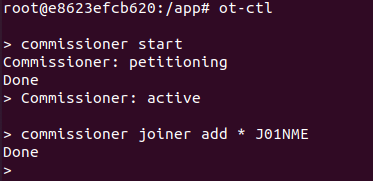
\includegraphics[width=0.8\linewidth]{graphics/screenshots/ot-ctl-commissioning.png}
    \caption{Zrzut ekranu konsoli OpenThread CLI, przedstawiający konfigurację roli Commissioner.}
    \label{fig:ctl-commissioner}
\end{figure}
    
Tak skonfigurowane urządzenie jest w pełni funkcjonalnym Ruterem brzegowym, pracującym w roli Commissioner.

W kolejnym kroku, uruchomiono pozostałe platformy nRF52833, pracujące jak urządzenia FTD\\ oraz HEATER i DIMMER. Po włączeniu urządzeń, przystąpiono do konfiguracji roli Joiner, każdego z węzłów.

Ukończywszy proces Commissioningu dokonano analizy powstałej topologi, dzięki której ustalono, że w sieci funkcjonują 2 węzły typu Dziecko, które pełnią role HEATER oraz DIMMER oraz 3 Rutery, z których jeden jest Liderem i Ruterem Brzegowym OTBR. Na potrzeby rozróżnienia 2 pozostałych Ruterów w dalszej części rozdziału, nadano im nazwę \textit{Router 1} oraz \textit{Router 2}. Następnie zweryfikowano połączenie między każdym węzłem sieci, rozsyłając pakiet ICMP (ang. \textit{Internet Control Message Protocol}) multicast na adres FF03::1, który jest subskrybowany przez każde urządzenie w danej sieci Thread. W Tabeli \ref{tab:mleid} zestawiono MLEID (ang. \textit{Mesh-Local Endpoint Identifiers}), czyli unikalne adresy IPv6 węzłów w utworzonej sieci Thread.

\begin{table}[H]
    \centering
    \caption{MLEID węzłów w sieci.}
    \begin{tabular}{|l|l|}
         \hline
         \rowcolor{gray!20}
         \multicolumn{1}{|c|}{Nazwa Węzła} & \multicolumn{1}{c|}{Adres IPv6} \\
         \hline
         OTBR & fd3f:cd2f:14fe:87f9:6b09:304e:878:6fb1 \\
         \hline
         HEATER & fd3f:cd2f:14fe:87f9:434d:bde5:7686:b429 \\
         \hline
         DIMMER & fd3f:cd2f:14fe:87f9:7998:c2a3:d56d:e3b0 \\
         \hline
         Router 1 & fd3f:cd2f:14fe:87f9:13a4:eced:d2c3:3922 \\
         \hline
         Router 2 & fd3f:cd2f:14fe:87f9:ce9e:4840:7dba:7356 \\
         \hline
    \end{tabular}
    \label{tab:mleid}
\end{table}


Upewniwszy się o poprawności funkcjonowania sieci oraz, że każde z urządzeń otrzymuje odpowiedź od pozostałych węzłów, uruchomiono aplikację System Controllera oraz Web GUI wykorzystując przygotowany wcześniej skrypt \textit{my-run-coap-server.sh} znajdujący się w repozytorium \cite{project-repo}. 

Topologię systemu po uruchomieniu wszystkich jego komponentów przedstawiono na Rysunku \ref{fig:system-topology}.

\begin{figure}[H]
    \centering
    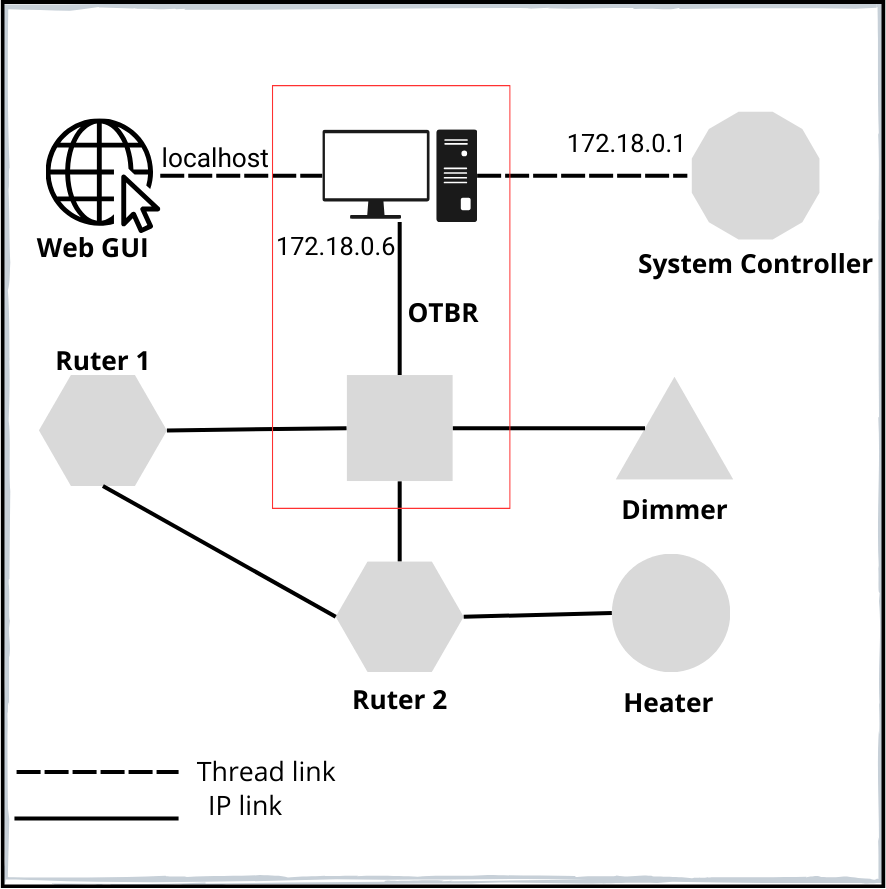
\includegraphics[width=0.8\linewidth]{graphics/system-topology.png}
    \caption{Topologia uruchomionego systemu.}
    \label{fig:system-topology}
\end{figure}

Ostatecznie włączono aplikację HEATER oraz DIMMER poprzez wciśnięcie przycisku Button 3 na obydwu urządzeniach. W efekcie zostało nawiązane połączenie klient-serwer między HEATER i DIMMER a System Controllerem.

Na Rysunku \ref{fig:serwer-app} zaprezentowano zrzut ekranu z konsoli, w której uruchomiono program System Controllera.

\begin{figure}[H]
    \centering
    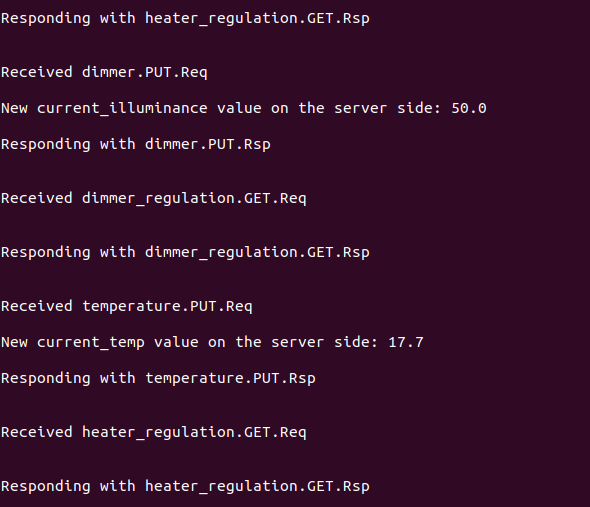
\includegraphics[width=0.8\linewidth]{graphics/screenshots/verification/system-controller-communication.png}
    \caption{Zrzut ekrany przedstawiający działanie System Controllera.}
    \label{fig:serwer-app}
\end{figure}

\section{Weryfikacja zasady działania systemu}

W celu weryfikacji poprawności zachowania stworzonego systemu, wykorzystano narzędzie Grafana \cite{grafana}. Platforma Grafana pozwala na tworzenie interaktywnych paneli do monitorowania danych z wybranego przez użytkownika źródła, takiego jak baza danych. Aby zwizualizować dane pochodzące z logów systemowych, jako zasób wybrano zaimplementowaną Bazę Danych, której architektura przedstawiono na Rysunku \ref{fig:db-diagram}. Następnie z wykorzystaniem kwerend SQL, utworzono panel Grafana zawierający 4 przebiegi czasowe, które przedstawiono na  na Rysunkach \ref{fig:graph-heater-temperature}, \ref{fig:graph-heater-regulation}, \ref{fig:graph-dimmer-illuminance} oraz \ref{fig:graph-dimmer-regulation}.
    
\begin{figure}[H]
    \centering
    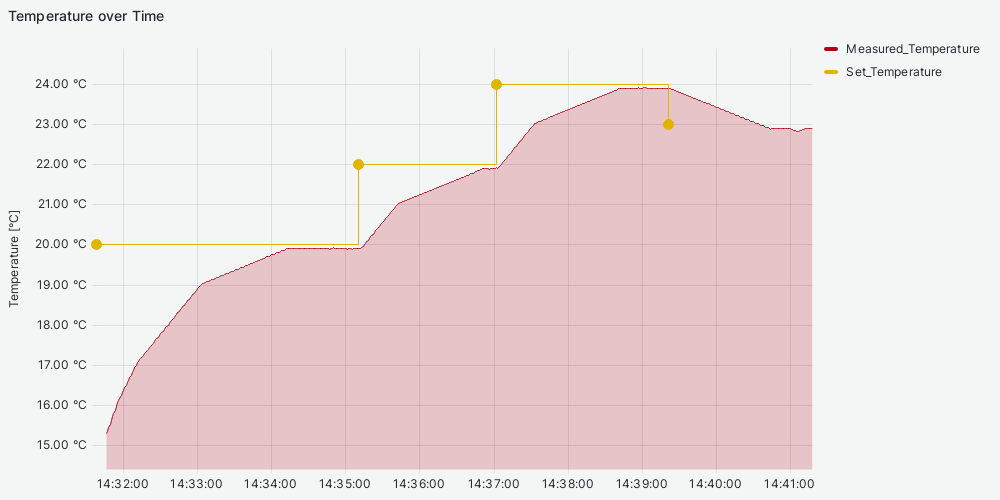
\includegraphics[width=0.8\linewidth]{graphics/grafana/temperature-lm.png}
    \caption{Przebiegi czasowe zmierzonej oraz ustalonej temperatury.}
    \label{fig:graph-heater-temperature}
\end{figure}

\begin{figure}[H]
    \centering
    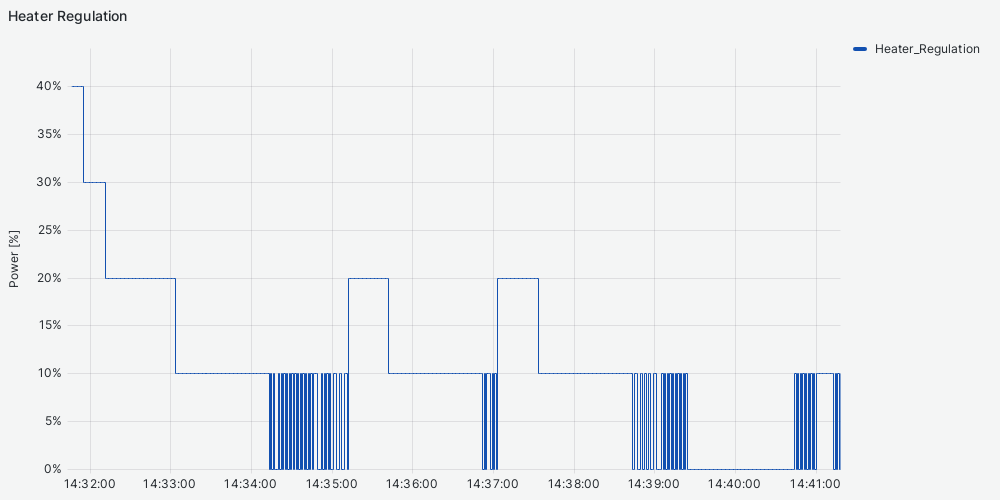
\includegraphics[width=0.8\linewidth]{graphics/grafana/heater-regulation-lm.png}
    \caption{Przebieg czasowy regulacji mocy układu HEATER.}
    \label{fig:graph-heater-regulation}
\end{figure}

\begin{figure}[H]
    \centering
    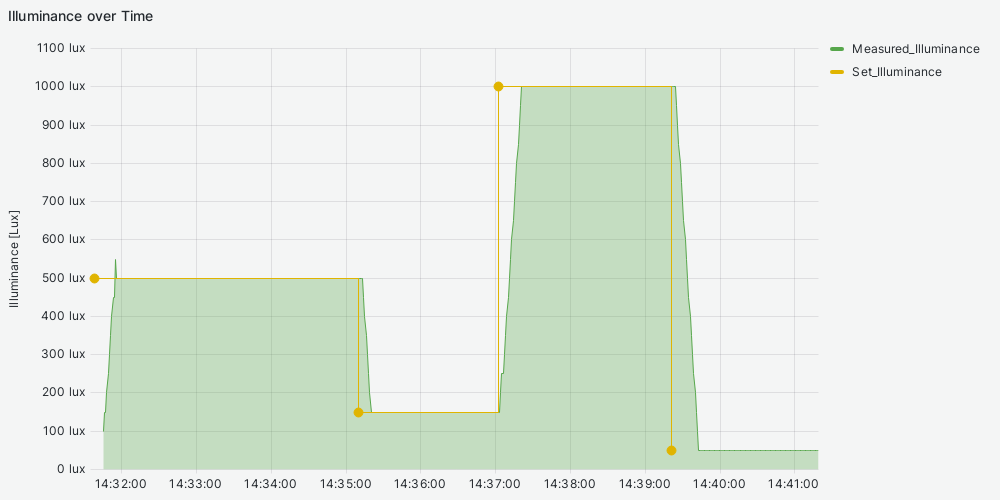
\includegraphics[width=0.8\linewidth]{graphics/grafana/illuminance-lm.png}
    \caption{Przebiegi czasowe zmierzonego oraz ustalonego natężenia oświetlenia.}
    \label{fig:graph-dimmer-illuminance}
\end{figure}

\begin{figure}[H]
    \centering
    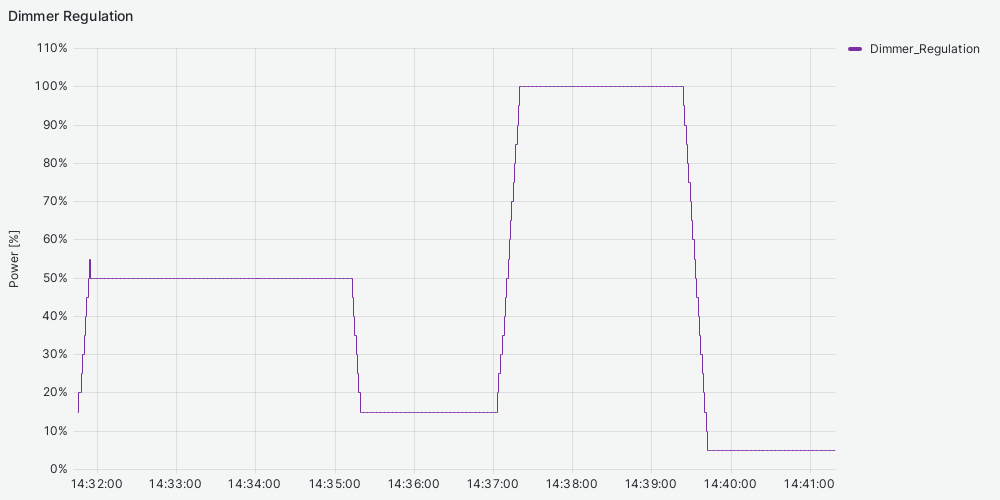
\includegraphics[width=0.8\linewidth]{graphics/grafana/dimmer_regulation-lm.png}
    \caption{Przebieg czasowy regulacji mocy układu DIMMER.}
    \label{fig:graph-dimmer-regulation}
\end{figure}
    
    Z przebiegów znajdujących się na Rysunku \ref{fig:graph-heater-temperature} oraz \ref{fig:graph-dimmer-illuminance} można zauważyć, że odpowiednio aktualna temperatura oraz natężenie oświetlenia zmierzają do ustalonej przez użytkownika wartości. Zobrazowane na Rysunkach \ref{fig:graph-heater-regulation} oraz \ref{fig:graph-dimmer-regulation} zmiany parametru regulacji pokrywają się ze zdefiniowanymi algorytmami w System Controllerze. Zatem, obserwując wszystkie 4 wymienione wykresy, można stwierdzić o poprawności działania systemu, względem poczynionych założeń.
\chapter{Analiza śladu pamięci}

W celu umożliwienia estymacji wymaganych zasobów sprzętowych w systemach opartych o protokół Thread, a w szczególności korzystających z implementacji OpenThread na platformie nRF52, dokonano badania, w którym analizowano stopień wykorzystania pamięci RAM oraz ROM (ang. \textit{Read-Only Memory}) po uruchomieniu stosu Thread oraz w zależności od wybranych funkcjonalności.

\section{Doświadczenie}

    \subsection{Założenia}

    Badanie przeprowadzono dla aplikacji dedykowanych platformie nRF52833 DK, stworzonych przy pomocy nRF Connect IDE. Do pomiarów wykorzystano narzędzia \textit{Memory Raport}, które jest częścią wspomnianego środowiska programistycznego. 
    
    W ramach analizy dokonywano modyfikacji stworzonego na potrzeby doświadczenia projektu, poprzez włączanie kolejnych funkcjonalności powiązanych ze stosem Thread. W kolejnym kroku porównywano zużycie RAM oraz ROM, dodatkowo wyszczególniając obszary pamięci, które zajmują najwięcej miejsca.

    Na Rysunku \ref{fig:memory-raport} przedstawiono zrzut ekranu prezentujący narzędzie Memory Raport.

    \begin{figure}[H]
        \centering
        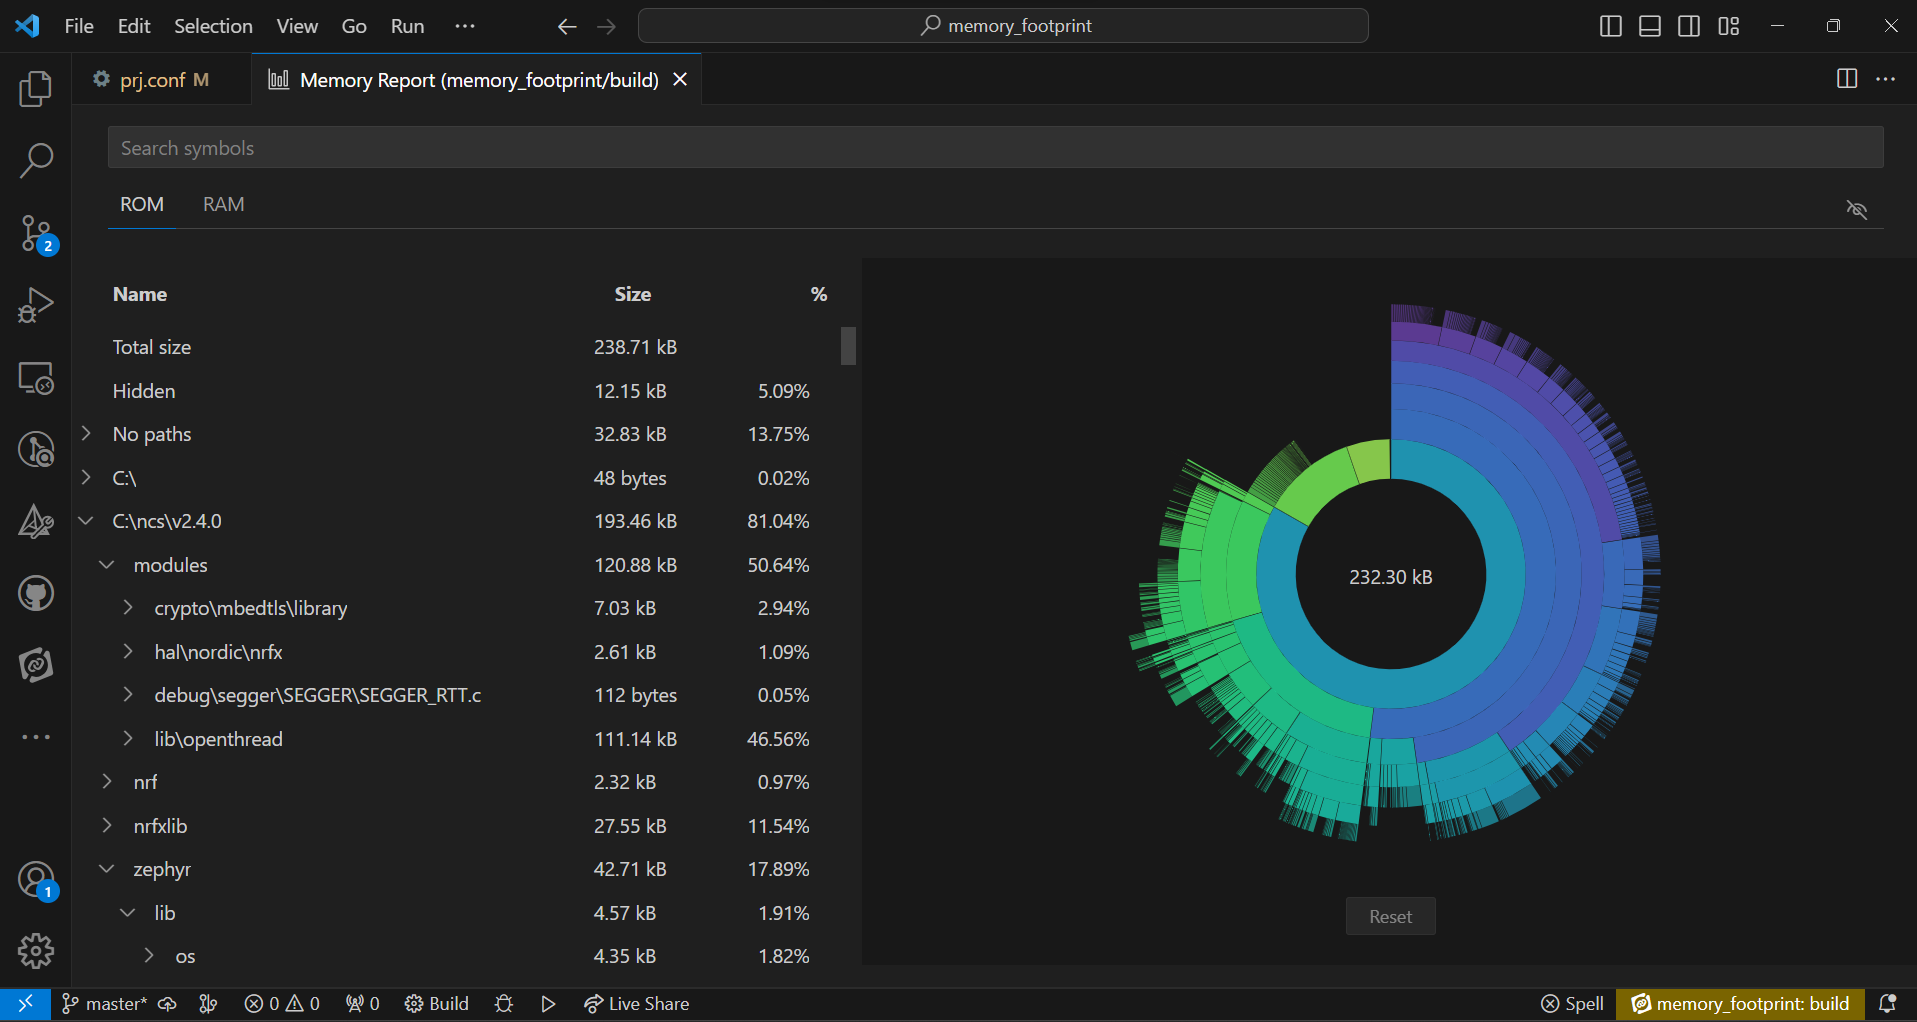
\includegraphics[width=0.8\linewidth]{graphics/memory-raport.png}
        \caption{Zrzut ekranu z narzędziem Memory Raport.}
        \label{fig:memory-raport}
    \end{figure}

    \subsection{Pomiar}
    \label{subsec:mem-footprint-measure}

        \subsubsection{Projekt bez dodatkowych konfiguracji}
        
        W celu ustalenia punktu odniesienia zbudowano projekt bez uwzględniania jakichkolwiek dodatkowych opcji konfiguracji.
        Uzyskane zużycie pamięci zestawiono na pozycji \textit{1} w Tabeli \ref{tab:memory-measures}.
        
        Zauważono, że większość wykorzystanego ROM związana jest z uruchomieniem systemu operacyjnego Zephyr i jest skojarzona z uwzględnieniem sterowników sprzętowych oraz warstwy HAL (ang. \textit{Hardware Abstraction Layer}). W przypadku pamięci RAM, większość zasobów została poświęcona na stos przerwań oraz na inicjalizację jądra systemu operacyjnego.

        \subsection{Projekt z opcją networking}

        Do inicjalizacji stosu Thread, niezbędnym jest skonfigurowanie warstwy sieciowej IP oraz funkcjonalności z nią związanych. W tym celu wzbogacono projekt o parametr konfiguracyjny \textit{CONFIG\_NETWORKING}, który uwzględnia w aplikacji warstwę łącza danych oraz warstwę sieciową z protokołem IP.
        Uzyskane zużycie pamięci zestawiono na pozycji \textit{2} w Tabeli \ref{tab:memory-measures}.

        \subsection{Projekt z włączonym stosem Thread v1.3}

        Po włączeniu warstwy sieciowej projekt jest przygotowany na wystartowanie protokołu Thread w implementacji OpenThread. Dodano do pliku konfiguracyjnego opcję \textit{CONFIG\_NET\_L2\_OPENTHREAD}, która konfiguruje LR-WPAN oraz uwzględnia funkcjonalności niezbędne do uruchomienia stosu Thread. Uzyskane zużycie pamięci zestawiono na pozycji \textit{3} w Tabeli \ref{tab:memory-measures}.

        Uwzględnienie stosu Thread spowodowało ponad czterokrotny wzrost zużycia ROM oraz niemalże czterokrotnie większe wykorzystanie RAM. 
        
        Najwięcej zasobów pamięci nieulotnej jest pochłanianych przez bibliotekę OpenThread, uwzględnioną przez nRF Connect SDK. Rozmiar sekcji pamięci przeznaczonej dla biblioteki OpenThread wynosi 94,01 kB. Stos Thread wymaga odbioru ramek IEEE 802.15.4. Obszar dedykowany dla sterowników do konfiguracji LR-WPAN zajął 27,31 kB.

        Wysokie zużycie RAM jest spowodowane koniecznością alokacji sekcji pamięci dla kontekstu sieci Thread, zastosowań kryptograficznych Mbed TLS oraz obsługi radia LR-WPAN. Sekcja przeznaczona na kontekst \textit{ot::gInstanceRaw} zajmuje 27,44 kB, natomiast obszar wykorzystywany przez Mbed TLS zużywa 12,92 kB.

    \subsection{Projekt z włączonym stosem Thread w wersji 1.1 oraz 1.2}

    W celu porównania zużycia zasobów sprzętowych między kolejnymi wersjami Thread dokonano pomiaru wykorzystania RAM oraz ROM również dla wersji 1.1 oraz 1.2., dodając do pliku konfiguracyjnego parametr \textit{CONFIG\_OPENTHREAD\_THREAD\_VERSION\_1\_1} lub \\ \textit{CONFIG\_OPENTHREAD\_THREAD\_VERSION\_1\_2}. Uzyskane zużycie pamięci zestawiono na pozycji \textit{4} oraz \textit{5} w Tabeli \ref{tab:memory-measures}.

    Niewielka różnica w wielkości wykorzystanych zasobów RAM oraz ROM między wersją 1.1 a 1.2, oraz 1.3 wynika z konieczności uwzględnienia dodatkowych mechanizmów i funkcjonalności w sieci Thread \cite{nrf-thread-version-options}, takich jak \textit{Coordinated Sampled Listening}, \textit{Link Metrics Probing}, \textit{Multicast across Thread networks}, \textit{Thread Domain unicast addressing}, \textit{Enhanced Frame Pending, Enhanced Keep Alive}.

    Ostatecznie, dla kolejnych rozważań, przywrócono konfigurację stosu Thread do wersji 1.3.

    \subsection{Projekt z włączonym stosem Thread dla różnych typów urządzeń}

    Domyślnym typem urządzenia dla skonfigurowanej aplikacji z włączonym stosem Thread jest FTD. W celu zbadania zużycia zasobów pamięci dla projektu, w którym urządzenie działa jako MTD, nadpisano konfigurację, dodając do pliku konfiguracyjnego parametr \textit{CONFIG\_OPENTHREAD\_MTD}. Co więcej, zmieniono konfigurację projektu, dodając opcję \textit{CONFIG\_OPENTHREAD\_MTD\_SED}, aby zbadać zmianę użytych zasobów dla urządzenia SED. Uzyskane zużycie pamięci zestawiono na pozycji \textit{6} oraz \textit{7} w Tabeli \ref{tab:memory-measures}.

    Można zauważyć, że przełączenie konfiguracji na MTD obniża zużycie zarówno ROM jak i RAM. Urządzenia typu MTD posiadają zredukowany zestaw funkcjonalności w sieci Thread, jak np. nie są w stanie przekazywać pakietów do innych węzłów. Potwierdza to zmniejszona, w stosunku do przypadku 5, sekcja pamięci nieulotnej, dedykowana dla biblioteki OpenThread, której rozmiar wynosi 64,07 kB, jak również redukcja rozmiaru kontekstu sieci \textit{ot::gInstanceRaw} do wielkości 18,48 kB.

    Na skutek dodania funkcjonalności SED, nie zmierzono zmian w zużyciu zasobów pamięci.

    Na koniec przywrócono w projekcie rolę FTD.

    \subsection{Projekt z włączonym stosem Thread oraz skonfigurowanym mechanizmem Commissioning}
    Projekt ze skonfigurowanym stosem Thread w wersji 1.3 wzbogacono o funkcjonalności związane z mechanizmem Commissioning. Do pliku konfiguracyjnego dodano opcję \\\textit{CONFIG\_OPENTHREAD\_COMMISSIONER}, aby ustalić rolę Commissioner urządzenia, a następnie \\\textit{CONFIG\_OPENTHREAD\_JOINER} w celu konfiguracji roli Joiner. Uzyskane wartości zużytej pamięci zestawiono na pozycji \textit{8} oraz \textit{9} w Tabeli \ref{tab:memory-measures}.
    
    Po dokonaniu pomiaru wyłączono mechanizm Commissioning.

    \subsection{Projekt z włączonym stosem Thread oraz ze skonfigurowaną konsolą OpenThread CLI}

    Aby umożliwić konfigurację urządzeń w sieci Thread poprzez użycie OpenThread CLI, niezbędne jest skonfigurowanie konsoli Shell. Utworzono nowy projekt, w którym skonfigurowano tylko konsolę. Zmierzono zużycie zasobów i zestawiono na pozycji \textit{10} w Tabeli \ref{tab:memory-measures}. Kolejno powrócono do projektu ze stosem Thread v1.3 dla urządzenia FTD, a następnie włączono funkcjonalności konsoli Shell oraz dodatkowo skonfigurowano OpenThread CLI. Wykorzystany RAM oraz ROM po uwzględnieniu w projekcie OpenThread CLI zestawiono na pozycji \textit{11} w Tabeli \ref{tab:memory-measures}.
        
    \begin{table}[H]
        \centering
        \caption{Zużycie zasobów pamięci dla kolejno omwaianych przypadków.}
        \begin{tabular}{|l|l|l|l|}
            \hline
            \rowcolor{gray!20}
            \multicolumn{1}{|c|}{l.p.} & \multicolumn{1}{c|}{ROM [kB]} & \multicolumn{1}{c|}{RAM [kB]} & \multicolumn{1}{c|}{Opis} \\
            \hline
            1 & 19,11 & 5,78 & Brak dodatkowych konfiguracji\\
            \hline
            2 & 51,39 & 18,81 & Konfiguracja L2 oraz L3 IP\\
            \hline
            3 & 217,18 & 72,76 & Stos Thread v1.3, FTD\\
            \hline
            4 & 217,18 & 72,76 & Stos Thread v1.2, FTD\\
            \hline
            5 & 211,20 & 71,46 & Stos Thread v1.1, FTD\\
            \hline
            6 & 177,44 & 63,80 & Stosu Thread v1.3, MTD\\
            \hline
            7 & 177,44 & 63,80 & Stos Thread v1.3, MTD, SED\\
            \hline
            8 & 251,26 & 76,84 & Stos Thread v1.3, FTD, Commissioner\\
            \hline
            9 & 245,96 & 76,52 & Stos Thread v1.3, FTD, Joiner\\
            \hline
            10 & 42,99 & 11,44 & Konfiguracja konsoli Shell\\
            \hline
            11 & 304,32 & 87,43 & Stos Thread v1.3, FTD Openthread CLI \\
            \hline
        \end{tabular}
        \label{tab:memory-measures}
    \end{table}

    W Tabeli \ref{tab:component-memory-usage} przedstawiono oszacowane wartości zużytych RAM oraz ROM dla analizowanych funkcjonalności, które zostały obliczone na podstawie różnic między wartościami zasobów umieszczonych w Tabeli \ref{tab:memory-measures}.

    \begin{table}[H]
        \centering
        \caption{Zużycie zasobów pamięci przez wybrane komponenty.}
        \begin{tabular}{|l|l|l|l|}
            \hline
            \rowcolor{gray!20}
            \multicolumn{1}{|c|}{Funkcjonalność} & \multicolumn{1}{c|}{ROM [kB]} & \multicolumn{1}{c|}{RAM [kB]} & \multicolumn{1}{c|}{Wymagana funkcjonalność} \\
            \hline
            Inicjalizacja Zephyr & 19,11 & 5,78 & brak\\
            \hline
            Networking & 32,28 & 13,03 & Inicjalizacja Zephyr\\
            \hline
            Konsola Shell & 23,88 & 5,66 & Inicjalizacja Zephyr\\
            \hline
            Stos Thread v1.3 dla FTD & 165,79 & 53,95 & Networking\\
            \hline
            Stos Thread v1.3 dla MTD & 126,05 & 44,99 & Networking\\
            \hline
            Rola Commissioner dla FTD & 40,06 & 4,08 & Stos Thread v1.3 dla FTD\\
            \hline
            Rola Joiner dla FTD & 28,16 & 3,76 & Stos Thread v1.3 dla FTD\\
            \hline
            OpenThread CLI dla FTD & 44,15 & 12,19 & Stos Thread v1.3 dla FTD, Konsola Shell\\
            \hline
        \end{tabular}
        \label{tab:component-memory-usage}
    \end{table}

\section{Wnioski}

Przeprowadziwszy analizę zużycia zasobów pamięci dla funkcjonalności protokołu Thread, na platformie nRF52833 w implementacji Openthread, wysunięto następujące wnioski.

Uruchomienie OpenThread wymaga dołączenia biblioteki, która w stosunku do innych wykorzystanych sekcji ROM, wymaga dużej liczby dostępnej pamięci nieulotnej. Nie jest możliwym na podstawie przeprowadzonej obserwacji, aby stwierdzić, czy uwzględnienie całej biblioteki załączonej do pamięci nieulotnej, jest niezbędne do poprawnego działania stosu Thread. Jeżeli w użytej bibliotece są zawarte fakultatywne funkcjonalności, istniałaby możliwość na optymalizację zużycia zasobów, poprzez selektywny dobór tylko tych funkcjonalności, który są konieczne do zapewnienia zgodnego ze standardem \cite{thread-1.3.0} działania sieci Thread.

Największe zużycie RAM spowodowane jest potrzebą zaalokowania w pamięci ulotnej obszaru dla kontekstu sieci Thread oraz zmiennych wykorzystywanych w zastosowaniach kryptograficznych. Domyślną biblioteką algorytmów szyfrowania, która została uwzględniona przy uruchomieniu OpenThread, jest Mbed TLS. W celu ewentualnej optymalizacji zużytych zasobów pamięci, sugerowane jest porównanie wykorzystanej implementacji z innymi, otwartymi, dostępnymi bibliotekami TLS (ang. \textit{Transport Layer Security}), takimi jak np. \textit{OpenSSL}, \textit{libsodium}, \textit{Crypto++} \cite{mbed-tls-alt}. 

Rola MTD wymaga mniejszych zasobów niż FTD. Urządzenia końcowe pracujące jako MED, pełniące rolę czujników i regulatorów, są w stanie posiadać mniejsze zasoby pamięci, niezbędne do poprawnego działania. Z kolei do uruchomienia urządzeń pracujących jako Rutery, konieczne jest uwzględnienie większego zaplecza pamięci. Ponadto włączenie roli Commissioner zużywa więcej RAM oraz ROM, aniżeli uruchomienie roli Joiner. Urządzeniem Commissioner może być tylko Ruter, co wprowadza dodatkowe wymagania odnośnie dostępnej pamięci.

W przypadku potrzeby wykorzystywania konsoli OpenThread CLI, zalecane jest, aby wykorzystać urządzenie o pamięci RAM oraz ROM większej o liczbę przedstawioną w Tabeli \ref{tab:component-memory-usage}. Włączenie konsoli OpenThread nie jest niezbędne, natomiast może być pomocna w przypadku chęci dynamicznej konfiguracji sieci Thread w trakcie działania aplikacji, szczególnie na takich urządzeniach jak Rutery czy Rutery Brzegowe.





\section*{Podsumowanie}

Co zostało zrobione

Future Work - czego nie zrobiono, a można by

Zakończenie, w miarę spójne ze wstępem, aby zrobić taką klamrę

\addcontentsline{toc}{section}{Podsumowanie}
\addcontentsline{toc}{section}{Bibliografia}
\printbibliography

\end{document}
